%\documentclass[10pt]{article}
%\usepackage[usenames]{color} %used for font color
%\usepackage{amssymb} %maths
%\usepackage{amsmath} %maths
%\usepackage[utf8]{inputenc} %useful to type directly diacritic characters
%


\documentclass[orivec]{llncs}
\usepackage[table]{xcolor}
\usepackage{amssymb}
%\usepackage{float}
%\usepackage{placeins}
\usepackage[most]{tcolorbox}
\newtcolorbox{mybox}[2][]{%
  attach boxed title to top center
               = {yshift=-10pt},
               %width=85mm,%
                  %height=52mm,
  %colback      = black,
  colframe     =black,
  %fonttitle    = \bfseries,
  colbacktitle = black,
  title        = #2,#1,
  enhanced,
}

\usepackage{pgfplots}
\usepackage{pgfplots, pgfplotstable}

\usepackage{hyperref}

\usepackage{float}
\newcommand{\st}{\scriptscriptstyle}
\newcommand{\mb}{\mathbf}
\newcommand{\resizeT}{\scalebox{1}}
\newcommand{\resizeS}{\scalebox{.6}}
\newcommand{\resizeSS}{\scalebox{.38}}
\newcommand{\ignore}[1]{}
\newcommand{\PRF}{\mathtt{PRF}}
\newcommand{\TZ}[1]{\textcolor{magenta}{\textbf{Thomas: }{#1}}}

\usepackage{boxedminipage}
\usepackage{enumitem}
\usepackage{makeidx}  % allows for indexgeneration
\usepackage{amsfonts,amsmath,amssymb,graphicx,setspace,tipx}
\usepackage{amsmath}
\usepackage{float}
\usepackage{amssymb}
\usepackage[ruled,linesnumbered]{algorithm2e}
\usepackage{subfig}
\usepackage{graphicx}
\usepackage{framed}
\usepackage{esvect}
\usepackage{tikz}
\usepackage{latexsym}

\usepackage{tikz}
\usepackage{pgfplots}
\usepackage{pgfplots, pgfplotstable}
\usepackage{blkarray}% http://ctan.org/pkg/blkarra
\usepackage{mathtools}
\usepackage{amsmath}
\usepackage{bm}
\usepackage{adjustbox}
\usepackage{blindtext}
\usepackage{multicol}
\usepackage[disable]{todonotes}
\usepackage{prettyref}
\newrefformat{fig}{Figure~\ref{#1}}
\newrefformat{apndx}{Appendix~\ref{#1}}
\newrefformat{equ}{Equation~\eqref{#1}}
\let\proof\relax
\let\endproof\relax
\usepackage{amsthm}
\makeatletter
\newtheorem*{rep@theorem}{\rep@title}
\newcommand{\newreptheorem}[2]{%
\newenvironment{rep#1}[1]{%
 \def\rep@title{#2 \ref{##1}}%
 \begin{rep@theorem}}%
 {\end{rep@theorem}}}
\makeatother
\newreptheorem{theorem}{Theorem}
\usepackage[title]{appendix}
\usepackage{multirow}
\usepackage{adjustbox}
\usepackage{blindtext}
\usepackage{multicol}
\usepackage{tablefootnote}

%%%%%
\newcounter{counter}


%%%%%
\usepackage{fullpage}

\begin{document}



%\title{Protecting Victims of \\ Authorised Push Payment Fraud}
%\title{Payment with Dispute Resolution: \\Protecting Authorised Push Payment Frauds' Victims}
\title{Payment with Dispute Resolution: \\ A Protocol For Reimbursing  Frauds' Victims}

\author{%
Aydin Abadi\thanks{aydin.abadi@ucl.ac.uk} and
Steven J. Murdoch\thanks{s.murdoch@ucl.ac.uk}}
\institute{University College London}

%\date{}
\maketitle{}


\begin{abstract}
An ``Authorised Push Payment'' (APP) fraud refers to the case where fraudsters deceive a victim to make payments to bank accounts controlled by them.  The total amount of money stolen via APP frauds is swiftly growing. Although regulators have provided guidelines to improve victims’ protection, the guidelines are vague and the victims are not receiving sufficient protection. To  \emph{facilitate victims' reimbursement}, in this work, we propose a protocol called  ``Payment with Dispute Resolution'' (PwDR) and formally define it. The protocol lets an honest victim prove its innocence to a third-party dispute resolver while preserving the protocol participants' \emph{privacy}. It makes black-box use of a standard online banking system. We evaluate its asymptotic cost and runtime via a prototype implementation. Our evaluation indicates that the protocol is efficient. It imposes only $O(1)$ overheads to the customer and bank.  Also, it takes a dispute resolver  $0.09$ milliseconds to settle a dispute between the two parties.
\end{abstract}


%!TEX root = main.tex


\section{Introduction}

An  ``Authorised Push Payment" (APP) fraud is a type of cyber-crime where a fraudster tricks a victim into making an authorised online payment into an account controlled by the fraudster. It is defined by the ``Financial Conduct Authority” (FCA) as \textit{``a transfer of funds by person $A$ to person $B$, other than a transfer initiated by or through person $B$, where: (1) $A$ intended to transfer the funds to a person other than $B$ but was instead deceived into transferring the funds to $B$; or (2) A transferred funds to $B$ for what they believed were legitimate purposes but which were in fact fraudulent''} \cite{FCA-Glossary}. The amount of money lost to  APP frauds is   substantial. According to  ``UK Finance" report,   only in the first half of 2021, a total of £$355.3$ million was lost to APP frauds, which has increased by  $71\%$  compared to losses reported in the same period in 2020; for the first time, the amount of money stolen via the APP frauds overtook even   card fraud losses \cite{2021-Half-Year-Fraud-Update}. The UK Finance report suggests that  online  payment is the type of payment method the victims used to make the authorised push payment in  $98\%$  of cases. The true cost of APP frauds often extends beyond the immediate financial loss,  to additional fees imposed by  investigating the event, remediation of internal banks' processes, and  dealing with the emotional fallout of the fraud. %The level of fraud in the UK is such that it is now a national security threat.


Although the amount of money lost to the App frauds and the number of cases have been significantly  increasing, the victims are not receiving  enough protection.   In the first half of 2021, only $42\%$ of the stolen funds returned to victims of  APP frauds \cite{2021-Half-Year-Fraud-Update}. Previous years had a lower rate than that. Despite   financial authorities and regulators have provided  guidelines to financial institutes to prevent  APP frauds occurrence and improve victims' protection, these guidelines are  ambiguous and    open to interpretation. Furthermore,  there exists  no  mechanism in place via which honest victims can  \emph{prove} their innocence. The APP frauds are not specific to the regular online banking systems, they will eventually find their way in other payment systems, such as cryptocurrency. To date, the APP fraud problem has been overlooked by the information security and cryptography research communities.


In this work, we formally define a scheme called ``Payment with Dispute Resolution'' (PwDR),  propose a protocol which instantiates it, and formally prove the protocol's security.  The PwDR lets an honest victim (of an APP fraud)  independently prove its innocence to a third-party dispute resolver, in order to be reimbursed.  We identify three crucial properties that a PwDR scheme should possess; namely, (a) security against a malicious victim: a malicious victim  which is not qualified for the reimbursement should not be reimbursed, (b) security against a malicious bank: a malicious bank should not be able to disqualify an honest victim  from being reimbursed, and (c) privacy: the customer’s and bank’s messages remain confidential from non-participants of the scheme, and a party which resolves dispute  learns as little information as possible.  The  protocol makes black-box use of a standard  online banking system, meaning that it does not require significant changes to the existing online banking systems and can rely on their security. It is accompanied by our lightweight threshold voting protocol, which can be of independent interest. We perform a rigorous cost analysis of the protocol via both asymptotic and runtime  evaluation (via a prototype implementation). Our cost analysis indicates that the protocol is indeed efficient. The customer's and bank's computation and communication complexity are constant, $O(1)$. It only takes $0.09$ milliseconds for a dispute resolver to settle a dispute between the two parties. We  make  the implementation source code publicly available. We hope that our result can serve as a foundation for further solutions to protect victims of this concerning  fraud. 



 


%We hope that our result can serve as a foundation for further solutions to protect an APP fraud victims and combat this type of fraud. 
  





\vspace{2mm}

\noindent\textbf{Summary of Our Contributions.} We (i) put forth the notion of Payment with Dispute Resolution (PwDR), identify its core security properties, and  formally define the PwDR, (ii) propose an efficient candidate construction  and formally prove its security, and (iii) perform a rigorous cost analysis of the construction.     





%!TEX root = main.tex

\section{Background}\label{sec::background}


%\subsection{Existing Guideline: Contingent Reimbursement Model Code}

Liability for  APP frauds has largely remained with  victims  that authorised the payment.  In the UK,  there have been  efforts  to protect the victims. In  2016, the UK's consumer protection organisation, called ``Which?'', submitted a super-complaint to the
 ``Financial Conduct Authority” (FCA) and  raised its concerns that despite the APP frauds victims' rate is  growing, the victims do not have enough protection \cite{Which?-super-complaint}.  Since then, the FCA has been collaborating with financial institutes  to develop several initiatives that
could  improve the response when they  occur. As a result,  the ``Contingent Reimbursement Model'' (CRM)  code  \cite{CRM-code} was proposed. This code  lays out a set of requirements and explains under which circumstances customers should be reimbursed by their  financial institutes when they fall victim to an APP fraud. So far,  there are at least nine firms, comprising nineteen brands (e.g., Barclays, HSBC,  Lloyds) signed up to the  code. 

%One of the tangible outcomes of the code is a service called ``Confirmation of Payee" (CoP)  offered by the CRM code signatories \cite{CoP}. This service checks the money recipient's account name, once it is inserted by the sender customer into the online banking platform. If there is not an exact match, CoP provides a warning to the  customers about the risks of making the payment. In the case where a customer ignores such a warning, makes a payment, and later falls to an APP fraud,  it may not be reimbursed, according to the CRM code.

Although the CRM code is a vital guideline  towards protecting  the frauds' victims, it is still  vague and open to interpretation. For instance, in 2020, the ``Financial Ombudsman Service'' (that settles complaints between consumers and businesses)  highlighted that firms  are applying the CRM code inconsistently and in some cases incorrectly, which resulted in failing to reimburse victims in cases anticipated by this code \cite{Financial-Ombudsman-Service-response}.  %As another example, one of the conditions in the CRM code that allows a bank to avoid reimbursing the customer is clause R2(1)(e) which states: \textit{``The Customer has been grossly negligent. For the avoidance of doubt the provisions of R2(1)(a)-(d) should not be taken to define gross negligence in this context''}.  Nevertheless, neither the CRM code  nor the ``Payment Services Regulations'' \cite{Regulations}   explicitly define under which circumstances the customer is considered ``grossly negligent'' in the context of  APP frauds. In particular, in the CRM code, the only terms that discuss customers' misbehaviour are  the provisions of R2(1)(a)-(d); however, as stated above, they should be excluded from the definition of the term gross negligence. On the  other hand,  in the Payment Services Regulations, this term is used three times, i.e.,  twice in regulation 75 and once in regulation 77. But in all  three cases, it is used for frauds related to \emph{unauthorised payments} which are  different types of frauds from  APP ones. Hence, there is a pressing need for an accurate solution to help and protect  APP frauds victims. 



Unlike the UK that has already recognised APP frauds and developed regulations for that,  the US's financial industry has not distinguished between APP fraud and other types of  fraud when labeling their overall fraud losses \cite{P20-report}. Thus, there exist no publicly available accurate reports and regulations concerning APP frauds provided by the financial industry in the US yet.\footnote{Although the FBI publishes  an annual internet crime report, e.g.,  \cite{internet-crime-report}, that includes some variants of APP fraud as well,  this report defines APP fraud's variants very broadly that can cover unrelated frauds too.  Also, it only captures the cases where victims directly reported  APP frauds' occurrence to the FBI; therefore, it excludes the cases where the victims reported the APP frauds' occurrence to their banks.}  To address the issue, in 2020, the Federal Reserve introduced the ``FraudClassifier Model'' which classifies payment frauds more granularly \cite{Fraud-Classifier}. It is yet to be seen how  regulations related to APP frauds  will be developed and how the payment industry will implement these regulations. Similarly, in the EU, there  exists no specific regulation developed 
%
%to protect APP frauds victims yet
%
%even the European regulation for electronic payment services, i.e., Payment Services Directive  (PSD),  has not been amended 
%
to explicitly capture APP frauds and protect the victims \cite{kjorven2020pays,McIlroy2021}.







%In the US, liability is still  left to the payer. 









% !TEX root =main.tex







\section{Preliminaries} \label{preliminaries}


\subsection{Informal Thread Model and Assumptions}\label{Notations-and-Assumptions}

The PwDR scheme consists of six types of parties. Below, we informally explain each type of party's role and the security assumption we make about each of them. We will provide a formal definition of the  PwDR scheme in Section \ref{sec::def}. 
%
\begin{itemize}
%
\item[$\bullet$] Customer $\mathcal{C}$: it is a regular customer of a bank. We call a customer  a victim after it falls victim to an APP fraud. We assume a victim is corrupted by a non-colluding active (or malicious) adversary. %; for instance, an unqualified victim  tries to make itself appear qualified for reimbursement. 
%
\item[$\bullet$] Bank $\mathcal{B}$: it is a regular bank that provides a standard online banking system. We assume it is corrupted by a non-colluding active adversary. We assume  any change to the source code of the online banking system is transparent and  can be detected. Note that in the real-world a bank is  not usually an active adversary and cares about its reputation, such as a ``rational'' or ``covert'' adversary which is weaker than the active one. However, to ensure our solution offers  a strong security guarantee, we assume the adversary is strong too, i.e., active one. 

%, e.g., the bank  uses a cryptographic commitment to commit to the source code. 
%
\item[$\bullet$] Smart contract $\mathcal{S}$: it is a standard  smart contract of a public  blockchain (e.g., Ethereum). It mainly acts as a tamper-proof public bulletin board to store different parties' messages.  We do not assume that a smart contract itself can offer any privacy. 
%
\item[$\bullet$] Certificate generator $\mathcal{G}$: it is a trusted third party (e.g., hospital, registry office) which provides signed digital certificates (e.g., certificate of death, divorce, disability) to customers. Its involvement is more implicit than the other  parties.
%
\item[$\bullet$]  A committee of arbiters $\{\mathcal{D}_{\st 1},..., \mathcal{D}_{\st n}\}$: it consists of  trusted third-party authorities, auditors, or regulators (e.g.,  financial conduct authority, prudential regulation authority, financial ombudsman service). Given a set of complaints, they compile the complaints    and provide  their binary verdicts. If needed, they are authorised to access the banking  system's backend software to carry out investigations. We assume all arbiters have interacted with each other once,  to agree on (a) a secret key, $\bar k_{\st 0}$, and (b) a pair of keys $({pk}_{\st\mathcal {D}}, {sk}_{\st\mathcal {D}})$  of an asymmetric key encryption.
%
\item[$\bullet$]  Dispute resolver $\mathcal{DR}$: it is an aggregator of arbiters' votes (e.g., public court). Given a collection of votes, it extracts and announces the final verdict. We assume it is corrupted by a non-colluding passive adversary. We assume $\mathcal C$ and $\mathcal B$  use a secure channel when they  send a message directly to $\mathcal{DR}$. 
%
\end{itemize}



\subsection{Notations}
We use $\mathtt{Enc}(.)$  and $\mathtt{Dec}(.)$ to denote the encrypting and decrypting algorithms of   a semantically secure symmetric key encryption scheme respectively. We also use  $\mathtt{ \tilde {Enc}}({pk}_{\st\mathcal {D}}, .)$ and   $\mathtt{\tilde{Dec}}({sk}_{\st\mathcal {D}}, .)$ to denote the encrypting and decrypting algorithms of   a semantically secure asymmetric key encryption scheme  which has  the following key generating algorithm:  $\tilde{\mathtt{keyGen}}(1^{\st\lambda})\rightarrow({sk}_{\st\mathcal {D}}, {pk}_{\st\mathcal {D}})$ and its  public key, ${pk}_{\st\mathcal {D}}$, is known to everyone.  We denote the banking system's internal payment  algorithm by  $\mathtt{pay}(.)$ that  transfers money from the customer's account to a payee's account that is specified by the customer.  We use $in_{\st p}$ to denote the inputs of this algorithm.  We also use $\phi$ to denote a null value. In Appendix \ref{sec:notation-table}, we provide a notation table. 


%We use $\mathtt{Enc}(.)$  and $\mathtt{Dec}(.)$ to denote the encrypting and decrypting algorithms of   a semantically secure symmetric key encryption scheme. In this work, we use a committee of honest arbiters $\mathcal{D}:\{\mathcal{D}_{\st 1},..., \mathcal{D}_{\st n}\}$. Each arbiter,  given a set of  inputs, provides a binary verdict.    We  assume  $\mathcal{D}_{\st i}$'s share a pair of keys $({pk}_{\st\mathcal {D}}, {sk}_{\st\mathcal {D}})$ of an asymmetric key encryption. The encryption scheme has  key generating  $\tilde{\mathtt{keyGen}}(1^{\st\lambda})\rightarrow({sk}_{\st\mathcal {D}}, {pk}_{\st\mathcal {D}})$,   encrypting $\mathtt{ \tilde {Enc}}({pk}_{\st\mathcal {D}}, .)$ and  decrypting $\mathtt{\tilde{Dec}}({sk}_{\st\mathcal {D}}, .)$ algorithms, where its public key is known to everyone.  Also, we assume all arbiters have interacted with each other to agree on a secret key, $\bar k_{\st 0}$.  In this work, a third party dispute resolver, $\mathcal{DR}$, is involved, which can be potentially semi-honest, i.e., a passive adversary. We assume bank and customer are potentially malicious, i.e., active adversary. We use $\phi$ to denote a null value.  Our proposed solution is built upon the existing online banking system. We assume the banking system has  algorithm  $\mathtt{pay}(.)$ that  transfers money from the customer's account to a payee's account that is specific by the customer.  We denote the inputs of this algorithm $in_{\st p}$. We assume the source code of the online banking system is static, and any change to the source code is transparent and  can be detected, e.g., the bank  uses a cryptographic commitment to commit to the source code. Moreover, we assume the online banking  system is secure. In Appendix \ref{sec:notation-table}, we provide a notation table. 





% Similar to the \emph{optimistic} fair cryptographic protocols that aim  at efficiency, e.g., in \cite{AsokanSW97,eurocrypt/AsokanSW98,BaoDM98,DongCCR13}, we assume the existence of a trusted third party arbiter   which remains offline most of the time but can be invoked to resolve a part of dispute. We emphasise that if the bank and customers behave honestly, then the arbiter is never involved. Even the (offline) presence of such an arbiter threatens adversarial behaviour and acts as a deterrence.  %The idea is akin to deterrence in criminology,  i.e.,  the threat of punishment will deter people from committing crimes.














\subsection{Digital Signature}\label{subsec:DS}

A digital signature is a scheme for verifying the authenticity of digital messages or documents. Below, we restate its formal definition, taken from \cite{DBLP:books/crc/KatzLindell2014}. 


\begin{definition}\label{sec::def}
A signature scheme  involves three algorithms, $\mathtt{Signature}:=(\mathtt{Sig.keyGen}, $ $\mathtt{Sig.sign}, \mathtt{Sig.ver})$, that are defined as follows.

\begin{itemize} 
\item[$\bullet$] $\mathtt{Sig.keyGen}(1^{\st \lambda})\rightarrow (sk,pk)$.  A probabilistic algorithm run by  a  signer. It takes as input a security parameter. It outputs a key pair: $(sk,pk)$, consisting of secret: $sk$, and public: $pk$ keys. 
\item[$\bullet$] $\mathtt{Sig.sign}(sk, pk, u)\rightarrow sig$. An algorithm run by the signer. It takes as input  key pair: $(sk,pk)$ and a message: $u$. It outputs a signature: $sig$.
\item[$\bullet$]  $\mathtt{Sig.ver}( pk, u, sig)\rightarrow h\in\{0,1\}$. A deterministic algorithm run by a verifier. It takes as input  public key: $pk$,  message: $u$, and signature: $sig$. It checks the signature's validity.   If the verification passes, then it outputs $1$; otherwise, it outputs $0$. 
\end{itemize}
\end{definition}

A digital signature scheme should meet the following properties:

\begin{itemize} 
\item[$\bullet$]  \textit{Correctness.} For every input $u$ it holds that:
%
$$Pr\Big[\  \  \mathtt{Sig.ver}( pk, u, \mathtt{Sig.sign}(sk, pk, u))=1\ : \
\mathtt{Sig.keyGen}(1^{\st \lambda})\rightarrow (sk, pk)  \Big]=1$$
%
\item[$\bullet$] \textit{Existential unforgeability under chosen message attacks.} A probabilistic polynomial time (PPT) adversary that obtains $pk$ and has access to a signing  oracle for messages of its choice, cannot create a valid pair $(u^{\st *},sig^{\st *})$ for a new message $u^{\st *}$  (that was never a query to the signing oracle), except with a small probability, $\sigma$. More formally: 




\small{
$$ \Pr\left[
  \begin{array}{l}
  
  u^{\st *}\not\in Q\ \wedge \\
   \mathtt{Sig.ver}( pk,  u^{\st *}, sig^{\st *}) =1\\
  
  
    
%(M(u^{\scriptscriptstyle *},k)\neq \sigma \lor Q(\text{aux},k)\neq q) \wedge\\ (a=1 \ \vee b=1)
\end{array} : 
    \begin{array}{l}
   
    \mathtt{Cer.keyGen}(1^{\st \lambda})\rightarrow (sk,pk) \\
  \mathcal{A}^{\mathtt{Sig.sign}(k,)}(pk)\rightarrow(u^{\st *}, sig^{\st *})

     
\end{array}    \right]\leq \mu(\lambda)$$
}
where $Q$ is the set of queries that $\mathcal{A}$ sent to the certificate generator oracle.
\end{itemize}



%
%An application of a digital signature is in digital certificate, which is a  document digitally signed  by a certificate generator. Given a certificate and its parameters,  anyone can check whether it has been correctly generated by a valid generator. There is a case  where 
%a \emph{hard copy} certificate is used.  In this case,  the process $\mathtt{Sig.keyGen}(.)$ outputs a blank legitimate stamped certificate as a private parameter: $sk$, and the description of a standard legitimate certificate as a public parameter: $pk$. Moreover, the process $\mathtt{Sig.sign}(k, u)$ takes $k$ and the file $u$ on which a certificate should be generated and outputs a stamped certificate with the information printed on it. The process $\mathtt{Sig.ver}( pk, u, sig)$ takes the public parameter, the file,  and the hard copy of the certificate and outputs $1$ if it is valid and $0$ if it is not. Note, when  a hard copy certificate is considered, it is not possible to precisely define the success probability of the adversary, as it depends on the technology available to the adversary to generate a blank stamped certificate that looks like a legitimate one. In the real world however, this probability is usually small (but it may not be negligible). In this paper, we mainly consider a digital certificate; however, our solution can adopt hard copy certificates as well with the above caveat  regarding the adversary's success probability. 



\subsection{Smart Contract}\label{subsec:SC} Cryptocurrencies, such as Bitcoin \cite{bitcoin} and Ethereum \cite{ethereum}, beyond offering a decentralised currency,  support  computations on  transactions. In this setting, often a certain computation logic is encoded in a computer program, called a \emph{``smart contract''}. Although Bitcoin, the first decentralised cryptocurrency, supports smart contracts, the functionality of Bitcoin's smart contracts is very limited, due to the use of the underlying programming language that does not support arbitrary tasks. To address this limitation, Ethereum, as a generic smart contract platform, was designed. Thus far, Ethereum has been the most predominant cryptocurrency framework that lets users define arbitrary smart. This framework allows users to create an account with a unique account number or address. Such users are often called external account holders, which can send (or deploy) their contracts to the framework’s blockchain. In this framework, a contract's code and its related data  are held by every node in the blockchain's network. Ethereum smart contracts are often written in a high-level Turing-complete programming language called ``Solidity''.The program execution's  correctness  is  guaranteed by the security of the underlying blockchain components. To prevent  a denial of service attack, the framework requires a transaction creator to pay a  fee, called \emph{``gas''}. %, depending on the complexity of the contract running on  it.  


% !TEX root =main.tex

\vspace{-2.2mm}


\subsection{Commitment Scheme}\label{subsec:commit}


A commitment scheme involves two parties,  \emph{sender} and  \emph{receiver}, and includes  two phases: \emph{commit} and  \emph{open}. In the commit phase, the sender  commits to a message: $x$ as $\mathtt{Com}(x,r)=\mathtt{Com}_{\scriptscriptstyle x}$, that involves a secret value,  $r$. In the open phase, the sender sends the opening $\ddot{x}:=(x,r)$ to the receiver which verifies its correctness: $\mathtt{Ver}(\mathtt{Com}_{\scriptscriptstyle x},\ddot{x})\stackrel{\scriptscriptstyle ?}=1$ and accepts if the output is $1$. Informally, a commitment scheme must satisfy two properties, (a) \textit{hiding}: it is infeasible for an adversary to learn any information about the committed  message, and (b) \textit{binding}: it is infeasible for an adversary to open a commitment  to different values  than the one  used in the commit phase. We provide more detail in Appendix \ref{subsec:commit-long}. 



% A commitment scheme involves two parties,  \emph{sender} and  \emph{receiver}, and includes  two phases: \emph{commit} and  \emph{open}. In the commit phase, the sender  commits to a message: $x$ as $\mathtt{Com}(x,r)=\mathtt{Com}_{\st x}$, that involves a secret value: $r\stackrel{\st\$}\leftarrow \{0,1\}^{\st\lambda}$. In the end of the commit phase,  the commitment $\mathtt{Com}_{\st x}$ is sent to the receiver. In the open phase, the sender sends the opening $\ddot{x}:=(x,r)$ to the receiver who verifies its correctness: $\mathtt{Ver}(\mathtt{Com}_{\st x},\ddot{x})\stackrel{\st ?}=1$ and accepts if the output is $1$.  A commitment scheme must meet two properties: (a) \textit{hiding}: it is infeasible for an adversary  to learn any information about the committed  message $x$, until the commitment $\mathtt{Com}_{\st x}$ is opened, and (b) \textit{binding}: it is infeasible for an adversary  to open a commitment $\mathtt{Com}_{\st x}$ to different values $\ddot{x}':=(x',r')$ than that was  used in the commit phase, i.e.,  to find  $\ddot{x}'$, \textit{s.t.} $\mathtt{Ver}(\mathtt{Com}_{\st x},\ddot{x})=\mathtt{Ver}(\mathtt{Com}_{\st x},\ddot{x}')=1$, where $\ddot{x}\neq \ddot{x}'$.  There exist efficient non-interactive  commitment schemes both in (a) the standard model, e.g., Pedersen scheme \cite{Pedersen91}, and (b)  the random oracle model using the well-known hash-based scheme such that committing  is : $\mathtt{H}(x||r)=\mathtt{Com}_{\st x}$ and $\mathtt{Ver}(\mathtt{Com}_{\st x},\ddot{x})$ requires checking: $\mathtt{H}(x||r)\stackrel{\st ?}=\mathtt{Com}_{\st x}$, where $\mathtt{H}:\{0,1\}^{\st *}\rightarrow \{0,1\}^{\st\lambda}$ is a collision resistant hash function; i.e., the probability to find $x$ and $x'$ such that $\mathtt{H}(x)=\mathtt{H}(x')$ is negligible in the security parameter, $\lambda$.
% !TEX root =main.tex



%\vspace{-3mm}
\subsection{Statement Agreement Protocol}\label{SAP}

Recently, a scheme called ``Statement Agreement Protocol'' (SAP)  has been proposed in \cite{cryptoeprint:2021:1145}. It   lets two mutually distrusted parties, e.g., $\mathcal{B}$ and $\mathcal{C}$, \emph{efficiently} agree on a private statement, $\pi$. Informally, the SAP  satisfies the following four properties: (1) neither party can convince a third-party verifier that it has agreed with its counter-party on a different statement than the one both parties previously agreed on, (2) after they agree on a statement,  an honest party can (almost) always prove to the verifier that it has the agreement, (3) the privacy of the statement is preserved (from the public), and (4) after both parties reach an agreement, neither can deny it.
%
%(1) neither party can convince  a third-party  verifier that it has agreed with its counter-party on a different statement than the one both parties previously agreed on, (2) after they  agree on a statement,  an honest party can (almost) always  prove to the verifier that it has the agreement, (3) the privacy of the statement is preserved (from the public), and (4) after both parties reach an agreement, neither can  deny it.  
%
The SAP uses a  smart contract and commitment scheme. It  assumes that each party  has a blockchain public address,  $adr_{\st\mathcal{R}}$ (where $\mathcal{R}\in\{\mathcal{B,C}\}$). Below, we restate  the  SAP, taken from \cite{cryptoeprint:2021:1145}. 


%
 \begin{enumerate}
 %
 \item\textbf{Initiate}. $\mathtt{SAP.init}(1^{\st\lambda}, adr_{\st\mathcal{B}}, adr_{\st\mathcal{C}}, \pi )$ 

 The following steps are taken   by  $\mathcal B$.
 
  \begin{enumerate}
  \item\label{SAP::deploy-contract}  Deploys a smart contract that  explicitly states both parties'  addresses, $adr_{\st\mathcal{B}}$ and  $adr_{\st\mathcal{C}}$. Let $adr_{\st\text{SAP}}$ be the deployed contract's address. 

   \item  Picks a random value $r$, and commits to the statement, $\mathtt{Com}(\pi, r)=g_{\st \mathcal{B}}$.
   \item Sends $adr_{\st\text{SAP}}$ and $\ddot{\pi}:=(\pi, r)$  to  $\mathcal C$, and $g_{\st\mathcal B}$ to the contract. 
   %\item Sends $g_{\st\mathcal C}$ to the contract, using its account. 
    \end{enumerate}
     
     \vspace{1mm}
     
    \item\textbf{Agreement}. $\mathtt{SAP.agree}(\pi, r, g_{\st \mathcal{B}}, adr_{\st\mathcal{B}}, adr_{\st\text{SAP}})$

     The following steps are taken   by  $\mathcal C$.
     %
     \begin{enumerate}
 %
   \item Checks  if $g_{\st \mathcal{B}}$ was  sent  from $adr_{\st \mathcal{B}}$, and checks locally $\mathtt{Ver}(g_{\st\mathcal B}, \ddot{\pi})=1$.
   %
   \item If the checks pass, it sets $b=1$,    computes locally $\mathtt{Com}(\pi, r)=g_{\st\mathcal C}$, and sends $g_{\st\mathcal C}$ to the contract. Otherwise, it sets $b=0$ and $g_{\st\mathcal C}=\bot$.
 %
   %\item  If $b=1$, then sends $g_{\st\mathcal S}$ to the contract. % using its account.
    \end{enumerate}
     
          \vspace{1mm}
     
   \item\textbf{Prove}. For either $\mathcal B$ or $\mathcal C$ to prove, it sends $\ddot{\pi}:=(\pi, r)$  to the smart contract. 
   
        \vspace{1mm}
   
 \item\textbf{Verify}. $\mathtt{SAP.verify}(\ddot{\pi}, g_{\st\mathcal B},g_{\st\mathcal C}, adr_{\st\mathcal{B}}, adr_{\st\mathcal{C}})$
 
 
 The following steps are taken   by  the smart contract.
   \begin{enumerate}
   
\item\label{SAP::check-adr} Ensures $g_{\st\mathcal B}$ and $g_{\st\mathcal C}$ were sent from   $adr_{\st \mathcal{B}}$ and  $adr_{\st \mathcal{C}}$  respectively. 
  
   \item\label{SAP::check-commit} Ensures $\mathtt{Ver}(g_{\st\mathcal B},\ddot{\pi})=\mathtt{Ver}(g_{\st\mathcal C},\ddot{\pi}) =1$.
   
   \item Outputs $s=1$, if the checks, in steps \ref{SAP::check-adr} and \ref{SAP::check-commit}, pass. It outputs $s=0$, otherwise.
    \end{enumerate}
 \end{enumerate}

  
  
  
  
%  \item\textbf{Agreement}.
%  \begin{enumerate}
%   \item $\mathcal S$ picks a random value: $r$, and commits to the statement: $\mathtt{H}(x||r)=g_{\st S}$
%   \item $\mathcal S$ sends $r$  to the client and sends $g_{\st\mathcal S}$ to the contract. 
%   \item $\mathcal C$ checks: $\mathtt{H}(x||r)\stackrel{?}=g_{\st \mathcal S}$. If the equation  holds, it computes $\mathtt{H}(x||r)=g_{\st\mathcal C}$
%   \item $\mathcal C$   stores $g_{\st\mathcal C}$ in the contract. 
%    \end{enumerate}
%   \item\textbf{Prove}. For either $\mathcal C$ or $\mathcal S$ to prove, it has agreement on $x$ with its counter-party, it sends $\mu=(x, r)$  to the contract. 
% \item\textbf{Verify}. Given $\mu$, the contract does the following. 
%   \begin{enumerate}
%
%   \item checks if $\mathtt{H}(x||r)=g_{\st\mathcal C}=g_{\st\mathcal S}$
%   \item outputs $1$, if the above equation holds; otherwise, it outputs $0$
%    \end{enumerate}
% \end{enumerate}



%
% \begin{enumerate}
% \item\textbf{Setup}.  Both parties agree on a  smart contract and deploy it, such that the parties public keys, $pk_{\st C}$ and $pk_{\st S}$, are encoded in the contract.
%
%  
%  \item\textbf{Agreement}.
%  \begin{enumerate}
%   \item The server picks a random value: $r$, and commits to the statement: $H(s||r)=y_{\st S}$.
%   \item The server sends $r$  to the client and sends $y_{\st S}$ to the contract. 
%   \item The client checks: $H(s||r)\stackrel{?}=y_{\st S}$. If the equation  holds, it computes $H(s||r)=y_{\st C}$.
%   \item The client   stores $y_{\st C}$ in the contract. 
%    \end{enumerate}
%   \item\textbf{Prove}. For either $C$ or $S$ to prove, it has agreement on $s$ with its counter-party, it sends $\mu=(s, r)$, in a signed transaction, to the contract. 
% \item\textbf{Verify}. Given $\mu$, the contract does the following. 
%   \begin{enumerate}
%   \item verifies the public keys related to  signatures of $y_{\st C}$ and $y_{\st S}$ match $pk_{\st C}$ and $pk_{ \st S}$ respectively.
%   \item checks if $H(s||r)=y_{\st C}=y_{\st S}$.
%   \item outputs 1, if the above equation holds; otherwise, it outputs 0.
%    \end{enumerate}
% \end{enumerate}
 
 %Note that the above protocol is one-off, which means after first party
 
 
 
 
 %In Appendix \ref{sec:Discussion-on-the-SAP}, we discuss the SAP's security and explain why naive solutions are not suitable.
 

 
 
 
 %The SAP protocol might be of independent interest. 
 
 
% \begin{remark}
% The verification algorithm can also be executed \emph{off-chain}. In particular, given  statement $\ddot{x}$, anyone can read $(g_{\st\mathcal C},g_{\st\mathcal S},adr_{\st\mathcal{C}}, adr_{\st\mathcal{S}})$ from the SAP contract and locally run $\mathtt{SAP.verify}(\ddot{x}, g_{\st\mathcal C},g_{\st\mathcal S},adr_{\st\mathcal{C}}, adr_{\st\mathcal{S}})$ to check the statement's correctness.  This relieves  the verifier from the  transaction  and contract's execution costs. 
% \end{remark}
% 
%  \begin{remark}
%One may simply let each party  sign the statement and send it to the other party, so later on each party can send both signatures to the contract which verifies them. However, this would not work,  as the party who first receives the other party's signature  may refuse  to send its  signature, that prevents the other party from proving that it has  agreed on the statement with its counter-party. Alternatively, one may want to use a protocol for a fair exchange of digital signature (or fair contract signing) such as \cite{BonehN00,DBLP:conf/fc/GarayJ02}. In this case, after both parties have the other party's signature, they can sign the statement themselves and send the two signatures to the contract which first checks the validity of both  signatures. Although this satisfies the above security requirements, it yields two main efficiency and practical issues: (a) it imposes very high computation costs, as  protocols for a fair exchange of signature involve generic zero-knowledge proofs and require a high number of modular exponentiations. And (b) it is impractical because protocols for fair exchange of signature protocol support only certain signature schemes (e.g., RSA, Rabin, or Schnorr) that are not directly supported by the most predominant  smart contract framework,  Ethereum, that only supports  Elliptic Curve Digital Signature Algorithm (EDCSA).
% \end{remark}







\subsection{Pseudorandom Function}


Informally, a pseudorandom function is a deterministic function that takes a key of length $\Lambda$ and an input; and outputs a value  indistinguishable from that of  a truly random function.  In this paper, we use the pseudorandom function:   $\mathtt {PRF}: \{0,1\}^{\st \Lambda}\times \{0,1\}^{\st *} \rightarrow  \mathbb{F}_p$, where $p$ is a large prime number, $|p|=\lambda$, and $(\Lambda,\lambda)$ are the security parameters. In practice, a pseudorandom function can be obtained from an efficient block cipher. We refer readers to \cite{DBLP:books/crc/KatzLindell2014} for a formal definition of a pseudorandom function.


\subsection{Bloom Filter}


A Bloom filter \cite{DBLP:journals/cacm/Bloom70} is a compact data structure that allows us to 
efficiently check an  element membership. It is an array of $m$ bits (initially all set to zero), that  represents $n$  elements. It is accompanied by $k$ independent hash functions. To insert an element, all the  hash values of the element are computed and their corresponding bits in the filter are set to $1$. To check an element membership, all its hash values are re-computed and checked whether all are set to $1$ in the filter. If all the corresponding bits are $1$, then the element is probably in the filter; otherwise, it is not. In Bloom filters,  it is possible that an element is not in the set, but the membership query indicates it is, i.e., false positives. In this work, we ensure that the false positive probability is negligible, e.g.,  $2^{\st - 40}$. Also, we require that a Bloom filter uses \emph{cryptographic} hash functions. In Appendix \ref{sec::bloom-filter-}, we explain how the Bloom filter's parameters can be set.

%Informally, a digital certificate's security requires that no one can generate a valid certificate that was not previously produced by the certificate generator. The security of a digital certificate relies on the security of the digital signature scheme used.  Below, we present the formal definition of the digital signature.



%In the case where a digital certificate is considered, then $\mathtt{Cer}$ definition is equivalent to the definition of a digital signature scheme. In this case, it holds $\sigma=neg(\lambda)$, where $neg$ is a negligible function and $\lambda$ is a security parameter. Now, we briefly explain the procedures' input/output when a hard copy certificate is considered.  The process $\mathtt{Cer.genPar}(.)$ outputs a blank legitimate stamped certificate as a private parameter: $sk$, and the description of a standard legitimate certificate as a public parameter: $pk$. Morevoer, the process $\mathtt{Cer.genCrt}(k, u)$ takes $k$ and the file $u$ on which a certificate should be generated and outputs a stamped certificate with the information printed on it. The process $\mathtt{Cer.verCrt}( pk, u, crt)$ takes the public parameter, the file,  and the hard copy of the certificate and outputs $1$ if it is valid and $0$ if it is not. In the case where a hard copy certificate is considered, it is not possible to precisely define the probability $\sigma$, as it depends on the technology available to the adversary to generate a blank stamped certificate that looks like a legitimate one. In the real world however, this probability is usually small (but it may not be negligible).




%\input{PoR-def}

 

%% !TEX root =main.tex

%\break

\clearpage

\section{Notations}\label{sec:notation-table}

We summarise our notations in Table \ref{table:notation-table}.


\begin{table*}[!htbp]
\begin{scriptsize}
\begin{center}
\footnotesize{
\caption{ \small{Notation Table}.}\label{commu-breakdown-party} 
\renewcommand{\arraystretch}{1}
\scalebox{1.1}{
% 1st table
\begin{tabular}{|c|c|c|c|c|c|c|c|c|c|c|c|c|c|} 

\hline 

\cellcolor{gray!15} \scriptsize \textbf{Symbol}&\cellcolor{gray!15} \scriptsize \textbf{Description}  \\
    \hline
    
     \hline

%Generic
%\multirow{25}{*}{\rotatebox[origin=c]{90}{\scriptsize \textbf{Generic}}}

 \cellcolor{white!20}\scriptsize$\mathtt{Enc}(.)$&\cellcolor{white!20}\scriptsize \text{Encryption algorithm of symmetric key encryption  }\\   
 %
  \cellcolor{gray!20}\scriptsize$\mathtt{Dec}(.)$&\cellcolor{gray!20}\scriptsize \text{Decryption algorithm of symmetric key encryption  }\\   
  %
  \cellcolor{white!20}\scriptsize${\tilde{\mathtt{Enc}}}(.)$&\cellcolor{white!20}\scriptsize \text{Encryption algorithm of asymmetric key encryption  }\\   
  %
  \cellcolor{gray!20}\scriptsize${\tilde{\mathtt{Dec}}}(.)$&\cellcolor{gray!20}\scriptsize \text{Decryption algorithm of asymmetric key encryption  }\\   
  %
    \cellcolor{white!20}\scriptsize$\tilde{\mathtt{keyGen}}(.)$&\cellcolor{white!20}\scriptsize \text{Key generator algorithm of asymmetric key encryption } \\
%
   \cellcolor{gray!20}\scriptsize${\mathtt{Sig.keyGen}}(.)$&\cellcolor{gray!20}\scriptsize \text{Key generator algorithm of digital signature scheme} \\
 %
\cellcolor{white!20}\scriptsize$\mathtt{verStat}(.)$ &\cellcolor{white!20}\scriptsize  Algorithm to determine $\mathcal{B}$'s message status \\ 
%
\cellcolor{gray!20}\scriptsize$\mathtt{checkWarning}(.)$ &\cellcolor{gray!20}\scriptsize  Algorithm to check a warning’s effectiveness \\ 
%
\cellcolor{white!20}\scriptsize$\mathtt{pay}(.)$ &\cellcolor{white!20}\scriptsize $\mathcal{B}$'s internal algorithm to transfers money\\   
%
 \cellcolor{gray!20}\scriptsize$\mathtt{Com}(.)$ &\cellcolor{gray!20}\scriptsize  Commitment's commit\\
  %
\cellcolor{white!20}\scriptsize$\mathtt{Ver}(.)$ &\cellcolor{white!20}\scriptsize  Commitment's verify\\   
%                    
\cellcolor{gray!20}\scriptsize$\mathtt{H}(.)$ &\cellcolor{gray!20}\scriptsize Hash function\\
%
\cellcolor{white!20}\scriptsize$\mathtt{PRF}(.)$ &\cellcolor{white!20}\scriptsize  Pseudorandom function \\ 
%
\cellcolor{gray!20}\scriptsize$\mathcal{C}$ &\cellcolor{gray!20}\scriptsize Customer  \\  
%
\cellcolor{white!20}\scriptsize$\mathcal{B}$ &\cellcolor{white!20}\scriptsize Bank  \\
%  
\cellcolor{gray!20}\scriptsize$\mathcal{D}_{\st 1},... , \mathcal{D}_{\st n}$ &\cellcolor{gray!20}\scriptsize Arbiters  \\  
%
\cellcolor{white!20}\scriptsize$\mathcal{DR}$ &\cellcolor{white!20}\scriptsize Dispute resolver  \\  
%
\cellcolor{gray!20}\scriptsize$\mathcal{S}$ &\cellcolor{gray!20}\scriptsize Smart contract  \\  
%
\cellcolor{white!20}\scriptsize$\mathcal{G}$ &\cellcolor{white!20}\scriptsize Certificate generator  \\  
%
\cellcolor{gray!20}\scriptsize{SAP} &\cellcolor{gray!20}\scriptsize  Statement agreement protocol\\ 
%
\cellcolor{white!20}\scriptsize{PVE} &\cellcolor{white!20}\scriptsize  Private verdict encoding protocol\\ 
%
\cellcolor{gray!20}\scriptsize{FVD} &\cellcolor{gray!20}\scriptsize  Final verdict decoding protocol\\ 
%
\cellcolor{white!20}\scriptsize{GPVE} &\cellcolor{white!20}\scriptsize  Generic private verdict encoding protocol\\ 
%
\cellcolor{gray!20}\scriptsize{GFVD} &\cellcolor{gray!20}\scriptsize  Generic final verdict decoding protocol\\ 
%
\cellcolor{white!20}\scriptsize$\oplus$ &\cellcolor{white!20}\scriptsize  XOR operator \\ 
%
\cellcolor{gray!20}\scriptsize$\Delta$ &\cellcolor{gray!20}\scriptsize  time parameter \\ 
%
\cellcolor{white!20}\scriptsize$add_{\st I}$ &\cellcolor{white!20}\scriptsize  Address of $I$\\ 
%
\cellcolor{gray!20}\scriptsize$aux, aux'$ &\cellcolor{gray!20}\scriptsize  Auxiliary information\\ 
%
\cellcolor{white!20}\scriptsize$\mathtt{BF}$ &\cellcolor{white!20}\scriptsize  Bloom filter\\ 
%
\cellcolor{gray!20}\scriptsize$z_{\st 1}$ &\cellcolor{gray!20}\scriptsize  $\mathcal{C}$'s complaint about $\mathcal{B}$'s message status\\ 
%
\cellcolor{white!20}\scriptsize$z_{\st 2}$ &\cellcolor{white!20}\scriptsize  $\mathcal{C}$'s complaint about a warning's effectiveness\\
% 
\cellcolor{gray!20}\scriptsize$z_{\st 3}$ &\cellcolor{gray!20}\scriptsize  $\mathcal{C}$'s complaint about payment message  inconsistency\\ 
%
 {   }\scriptsize$t_{\st i}$ &\scriptsize  time point\\ 



                     
 \hline
  


\end{tabular}

% 2nd table
\begin{tabular}{|c|c|c|c|c|c|c|c|c|c|c|c|c|c|} 
    \hline
\cellcolor{gray!15} \scriptsize \textbf{Symbol}&\cellcolor{gray!15} \scriptsize \textbf{Description}  \\
    \hline
    
\hline


%---------------------------------
%\multirow{10}{*}{\rotatebox[origin=c]{90}{\scriptsize  \textbf{Generic}}}
%

\cellcolor{gray!20}\scriptsize$\bm{l}$ &\cellcolor{gray!20}\scriptsize  $\mathcal{C}$'s payees list\\ 
%
\cellcolor{white!20}\scriptsize$\hat{\bm{l}}$ &\cellcolor{white!20}\scriptsize  $\mathcal{C}$'s encoded payees list\\ 
%


\cellcolor{gray!20}\scriptsize$ k_{\st 0}$ &\cellcolor{gray!20}\scriptsize   A secret key of $\mathtt{PRF}$\\ 
%               
\cellcolor{white!20}\scriptsize$f$ &\cellcolor{white!20}\scriptsize New payee’s detail  \\ 
 %                            
\cellcolor{gray!20}\scriptsize$in_{\st f}$ &\cellcolor{gray!20}\scriptsize Payment detail \\ 
%
  \cellcolor{white!20}\scriptsize$\hat a$ &\cellcolor{white!20}\scriptsize Encoded $a$ \\     
%
\cellcolor{gray!20}\scriptsize$\hat {m}^{\st(\mathcal{C})}_{\st 1}$ &\cellcolor{gray!20}\scriptsize $\mathcal{C}$'s encoded update request\\     
%
\cellcolor{white!20}\scriptsize$\hat {m}^{\st(\mathcal{C})}_{\st 2}$ &\cellcolor{white!20}\scriptsize $\mathcal{C}$'s encoded payment request\\     
%      
\cellcolor{gray!20}\scriptsize$\hat {m}^{\st(\mathcal{B})}_{\st 1}$ &\cellcolor{gray!20}\scriptsize $\mathcal{B}$'s encoded warning message\\     
%
\cellcolor{white!20}\scriptsize$\hat {m}^{\st(\mathcal{B})}_{\st 2}$ &\cellcolor{white!20}\scriptsize $\mathcal{B}$'s encoded payment message\\     
%          
     \cellcolor{gray!20}\scriptsize$sk$ and $pk$ &\cellcolor{gray!20}\scriptsize Secret  and public keys\\     
%
   \cellcolor{white!20}\scriptsize$sk_{\st\mathcal{D}}$ &\cellcolor{white!20}\scriptsize Arbiters' secret key\\     
%    
\cellcolor{gray!20}\scriptsize$pp$ &\cellcolor{gray!20}\scriptsize Public parameter\\  
%
\cellcolor{white!20}\scriptsize$j$ &\cellcolor{white!20}\scriptsize  Arbiter's index,  $1\leq j\leq n$ \\ 
%
\cellcolor{gray!20}\scriptsize$T, T_{\st 1},T_{\st 2}$ &\cellcolor{gray!20}\scriptsize  Tokens, where  $T:=( T_{\st 1},T_{\st 2})$\\ 
%
\cellcolor{white!20}\scriptsize$w_{\st 1}$ &\cellcolor{white!20}\scriptsize  Output of $\mathtt{verStat}(.)$\\ 
%
\cellcolor{gray!20}\scriptsize$(w_{\st 2},w_{\st 3})$ &\cellcolor{gray!20}\scriptsize  Output of $\mathtt{checkWarning}(.)$\\ 
%
\cellcolor{white!20}\scriptsize$\bar{w}_{\st j}$ &\cellcolor{white!20}\scriptsize  Output of $\mathtt{PVE}(.)$\\ 
%
\cellcolor{gray!20}\scriptsize$v$ &\cellcolor{gray!20}\scriptsize  Output of $\mathtt{FVD}(.)$\\ 
%
\cellcolor{white!20}\scriptsize$e$ &\cellcolor{white!20}\scriptsize  Threshold\\ 
%            
 \cellcolor{gray!20}\scriptsize$w_{\st i,j}$ &\cellcolor{gray!20}\scriptsize  Arbiter's plain verdict\\ 
%     
\cellcolor{white!20}\scriptsize$o$ &\cellcolor{white!20}\scriptsize  Offset\\  
 %
  \cellcolor{gray!20}\scriptsize$r_{\st j}$ &\cellcolor{gray!20}\scriptsize  Pseudorandom value\\   
 %              
\cellcolor{white!20}\scriptsize$\lambda$ &\cellcolor{white!20}\scriptsize Security parameter\\  
%
\cellcolor{gray!20}\scriptsize$\mu$ &\cellcolor{gray!20}\scriptsize Negligible function\\  


\cellcolor{white!20}\scriptsize$in_{\st p}$ &\cellcolor{white!20}\scriptsize The input of $\mathtt{pay}(.)$\\                    
%
\cellcolor{gray!20}\scriptsize$\pi$ &\cellcolor{gray!20}\scriptsize Private statement\\        
  %
  \cellcolor{white!20}\scriptsize$Pr$ &\cellcolor{white!20}\scriptsize Probability\\   

%
\cellcolor{gray!20}\scriptsize$\phi$ &\cellcolor{gray!20}\scriptsize  Null\\ 
%
\cellcolor{white!20}\scriptsize$n$ &\cellcolor{white!20}\scriptsize  Total number of arbiters\\  
%           
\cellcolor{gray!20}\scriptsize$z$ &\cellcolor{gray!20}\scriptsize  $\mathcal{C}$'s complaint, where $z:=(z_{\st 1}, z_{\st 2}, z_{\st 3})$\\ 
%
\cellcolor{white!20}\scriptsize $g:=(g_{\st 1}, g_{\st 2})$&\cellcolor{white!20}\scriptsize  Commitment values \\    
%
%***********************

\hline 
      

           
              
\end{tabular}\label{table:notation-table}
%
}}
\end{center}
\end{scriptsize}
\end{table*}








%%%%%%%%%%%%%%%%%%%%%%%%%%%%%%%%%%%%%%%%%%%
























%!TEX root = main.tex

%\section{Notations and Assumptions}
%
%
%
%
%
%
%There are three main algorithms involved in the protocol; namely, $\mathtt{setupNewPayee}(.)$, $\mathtt{ammendExistingPayee}(.)$, and $\mathtt{pay}(.)$.
%The first two algorithms are executed by a smart contract while the third one is executed off-chain by a bank. We denote the inputs of algorithms $\mathtt{setupNewPayee}(.), \mathtt{ammendExistingPayee}(.)$, and $\mathtt{pay}(.)$ by $in_{\st s}, in_{\st a}$, and $in_{\st p}$ respectively. A null value is denoted by $\phi$. To determine the effectiveness of a warning we define a deterministic function   $\mathtt{f}(v_{\st 1}, ..., v_{\st n})\rightarrow b$  that takes $n$ binary inputs (or verdicts)  and outputs a binary value, $b$. For the sake of simplicity, we let this function output $1$ if the majority of the inputs are $1$; otherwise, it outputs $0$.  If $b=1$, it is said the warning is effective; otherwise (i.e.,   $b=0$), it is not effective. We assume the source code of the online banking system is static, is not updated, and any change to the source code can be detected (e.g., the bank can use a cryptographic commitment to commit to the source code). Moreover, we assume the online banking  system is secure.  %Moreover, we assume a customer does not collude with the APP scammer. 

%In our scheme, the bank requires to send a confirmation message to the smart contract after it transfers the customer's money. Since the transfer of money is performed off-chain, there is a possibility that  disputes occur between   the customer and bank in the case where there is an inconsistency between the money transfer and the confirmation (e.g., the bank transferred the money but did not send the confirmation). To allow such dispute to be resolved, we define a deterministic function   $\mathtt{madePayment}(w_{\st 1}, ..., w_{\st n})\rightarrow d$,  which takes $n$ binary verdicts of arbiters and outputs a binary value, $d$. This function outputs $1$ if the majority of the inputs are $1$; otherwise, it outputs $0$.  If $d=1$, it is said the payment has been made; otherwise (i.e.,   $d=0$), it has not been made. We assume the source code of the online banking system is static, is not updated, and any change to the source code can be detected (e.g., the bank can use a cryptographic commitment to commit to the source code).






% !TEX root =main.tex


\section{An Overview of Payment with Dispute Resolution Scheme}

In this section, we provide an overview of a Payment with Dispute Resolution (PwDR) scheme. Simply put, a PwDR scheme  allows a customer to interact with its bank (via the online banking scheme) to transfer a certain amount of money from its account to another account in a transparent manner; meanwhile, it  offers a distinct  feature. Namely, when an APP fraud takes place, it lets an honest customer raise a dispute and \emph{prove} to a third-party dispute resolver that it has acted honestly, so it can be reimbursed. It offers other features too. Specifically,  an honest bank can also prove it has acted honestly. PwDR lets the parties prove their innocence  without their counter-party's collaboration. It also ensures the message exchanged between a bank and customer remains confidential and even the party which resolves the dispute between the two learns as little information as possible.  The PwDR scheme can be considered as an extension to the existing   online banking system. To design such a scheme, we need to address  several challenges. The rest of this section  highlights these challenges. 



%\noindent\textit{Challenge 1: Lack of Transparent Logs.} 

\subsection{Challenge 1: Lack of Transparent Logs} 
In the current online  banking system, during a payment journey, the messages exchanged between customer and bank is usually logged by the bank and is not accessible to the customer without the bank's collaboration. Even if the bank provides access to the transaction logs, there is no guarantee that the logs have remained intact. Due to the lack of a transparent logging mechanism, a customer or bank can wrongly claim that (a) it has sent a certain message or warning to its counter-party or (b) it has never  received a certain message, e.g., due to hardware or software failure.  Thus, it would be hard for an honest party (especially a customer) to prove its innocence. To address this challenge, the PwDR protocol uses a standard smart contract (as a public bulletin board) to which  each party needs to send (a copy of) all outgoing messages, e.g., payment requests, warnings, and  confirmation of payments. 




\subsection{Challenge 2: Lack of Effective Warning's Accurate Definition in Banking}

One of the determining  factors in the process of allocating liability to the customers (after an APP fraud occurs) is paying attention to and following ``warning(s)'', according to the ``Contingent Reimbursement Model'' (CRM) code \cite{CRM-code}. However, there exists  no  publicly available study  on the  effectiveness of every warning used and provided by the bank. Therefore, we cannot hold a customer accountable for becoming the fraud's victim,  even if the related warnings are ignored.    To address this challenge, we let a warning's effectiveness is determined on a case-by-case basis after the fraud takes place. In particular, the protocol provides an opportunity to a victim to  challenge a certain warning whose effectiveness will be assessed by a committee, i.e., a small set of arbiters. In this setting, each member of the  committee provides (an encoding of) its verdict to the smart contract, from which a dispute resolver retrieves all verdicts to find out the final verdict. The scheme ensures that the final verdict is  in the customer's favour if at least threshold of committee members voted so. 

%that determine which runs a function on all verdicts and determines the warning's effectiveness. 




%\noindent\textit{Challenge 3: Linking Off-chain Payments with the Smart Contract.}


\subsection{Challenge 3: Linking Off-chain Payments with a Smart Contract}\label{sec::Linking Off-chain-Payments-with-contract}
 Recall that an APP fraud occurs when a payment is made. In the case where a  bank  sends a message (to the smart contract) to  claim  that it has transferred the money following the customer's request, it is not possible to automatically validate such a claim (e.g.,  for the smart contract doe the  check) as the money  transfer takes place  outside of the blockchain network. To address this challenge, the protocol lets a customer raise a dispute and report it to the smart contract when it detects an inconsistency (e.g., the bank did not transfer the money but it wrongly declared it did so, or when it transferred the money but did not declare it). In this case, the above committee members investigate and provide their  verdicts to the smart contract that allows the dispute resolver to extract the final verdict. 


%\noindent\textit{Challenge 4: Preserving Privacy.}

\subsection{Challenge 4: Preserving Privacy}
 Although the use of a public transparent logging mechanism plays a vital role in resolving disputes, if no  privacy-preserving mechanism is used, then it can violate parties' privacy, e.g., the customers' payment detail,  bank's messages to the customer, or even each arbiter's verdict. To protect the  privacy of the bank's and customers' messages against the public (and other customers), the PwDR scheme lets the customer and bank provably agree on encoding-decoding tokens that let them to encode their outgoing messages (sent to the smart contract). Later, either party can provide the token to a third party which can independently check the tokens' correctness, and decode the messages. To protect the privacy of the committee members' verdicts from the  dispute resolver, the PwDR scheme must ensure that  the dispute resolver can learn only the final verdict without being able to link a verdict to a specific  member of the committee. 

\input{Definition}




\vspace{-3mm}
\section{Payment with Dispute Resolution Protocol}\label{sec::PwDR-Protocol}

%In this section, first we  provide an outline of the PwDR protocol. %Then, we present a few subroutines that will be used in this protocol. After that, we describe the PwDR protocol in detail. 



\subsection{An Overview of  the PwDR Protocol}


In this section, we provide an overview of the  PwDR protocol. Initially, only  once    $\mathcal{C}$ and   $\mathcal{B}$   agree on a smart contract  $\mathcal{S}$. They also use the SAP to provably agree on two private statements that include two  secret keys that  will be used to encrypt outgoing messages. When $\mathcal{C}$ wants to transfer money to a new payee, it   signs into its online banking system.  It generates an update  request that specifies the new payee's detail,  encrypts the request, and sends the result to  $\mathcal{S}$. After that, $\mathcal{B}$ decrypts and checks the request's validity, e.g.,  whether it  meets its internal policy. Depending on the  request's content, $\mathcal{B}$ generates a pass or warning message. It encrypts the message and sends the result to $\mathcal{S}$. Then, $\mathcal{C}$ checks $\mathcal{B}$'s message, and depending on its content, decides whether  to   make  payment. If it decides to do so, then it sends an encrypted payment detail to $\mathcal{S}$. Next, $\mathcal{B}$  decrypts the message and locally transfers the amount of money specified in $\mathcal{C}$'s message. Once the money is transferred, $\mathcal{B}$ sends an encrypted  ``paid" message to $\mathcal{S}$. 


%Initially, the customer  $\mathcal{C}$ and bank  $\mathcal{B}$   agree on a smart contract  $\mathcal{S}$. They also use SAP to provably agree on two private statements; each statement includes a secret key, one is used to encrypt  messages that should be decrypted by all parties except $\mathcal{DR}$ and the other one is used to encrypt  messages that are supposed to be decrypted by $\mathcal{DR}$. For the sake of simplicity, we assume $\mathcal{C}$ wants to transfer a certain amount of money to a new payee. To do so, it   signs into the standard online banking system.  It generates an update  request that specifies the new payee's detail, it encrypts the request and sends the result to  $\mathcal{S}$. After that, $\mathcal{B}$ decrypts and checks this request's validity, e.g.,  whether it  meets its internal policy or  the requirements of the Confirmation of Payee (CoP) \cite{CoP}. Depending on the  request's content, $\mathcal{B}$ generates a pass or warning message. It encrypts the message and sends the result to $\mathcal{S}$. Then, $\mathcal{C}$ checks $\mathcal{B}$'s message and depending on the content of this message, it decides whether it wants to proceed to made  payment. If it decides to do so, then it sends an encrypted payment detail to $\mathcal{S}$. This  allows $\mathcal{B}$ to decrypt the message and locally transfer the amount of money specified in $\mathcal{C}$'s message. Once the money is transferred, $\mathcal{B}$ sends encrypted  ``paid" message to $\mathcal{S}$. 






%When it decides to invoke either  (a) algorithm $\mathtt{setupNewPayee}(.)$ to setup a new payee, or (b) algorithm $\mathtt{ammendExistingPayee}(.)$ to modify the existing payee's detail,  it sends the inputs of the related algorithm to $\mathcal{S}$ which runs the associated algorithm.  



%After a fixed time period, $\mathcal{B}$ checks the validity of the inputs that are registered by $\mathcal{C}$ in $\mathcal{S}$.  If the check fails (e.g., the input does not meet  the requirements of the Confirmation of Payee \cite{CoP}), then it sends  to $\mathcal{S}$ a warning message that includes the waring's detail; otherwise, it sends to $\mathcal{S}$ the ``pass'' message. Note that  $\mathcal{C}$ comes across with the same warning when it interacts with the online payment system's user interface.   Depending on the content of $\mathcal{B}$'s message, $\mathcal{C}$ decides whether it wants to proceed to made  payment. If it decides to make payment, then it sends the payment's detail to $\mathcal{S}$. This  allows $\mathcal{B}$ to locally transfer the amount of money specified in $\mathcal{C}$'s message. 


%Once the money is transferred, $\mathcal{B}$ sends the message ``paid" to $\mathcal{S}$. 


Once $\mathcal{C}$ realises that it has fallen victim, it  raises a dispute. In particular, it  generates  an encrypted complaint that could  challenge the effectiveness of the warning and/or any payment inconsistency. It can   include in the complaint an  evidence/certificate, e.g., asserting that it falls into  the vulnerable customer category as defined in the CRM code. $\mathcal{C}$ encrypts the complaint and  sends to $\mathcal{S}$ the result and a proof asserting the secret key's correctness.  Then, each committee member verifies the proof. If the verification passes, it decrypts and compiles $\mathcal{C}$'s complaint to generate a (set of) verdict. Each committee member encodes its verdict and sends the   encoded verdict's encryption to $\mathcal{S}$. To resolve a dispute between $\mathcal{C}$ and $\mathcal{B}$, either of them can  invoke $\mathcal{DR}$. To do so, they  directly send to it one of the above secret keys and a proof asserting that key was generated correctly.   $\mathcal{DR}$ verifies the proof. If the verification passes, it locally decrypts the encrypted encoded verdicts (retrieved from $\mathcal{S}$) and then combines the result to find out the final verdict.  If the final verdict indicates the legitimacy of  $\mathcal{C}$'s complaint, then $\mathcal{C}$ must be reimbursed.   Note, the verdicts are encoded in  a way that even after decrypting them, $\mathcal{DR}$ cannot link a verdict to a committee member or even figure out how many $1$ or $0$ verdicts were provided  (except when all verdicts are $0$). However, it can find out whether at least threshold committee members voted  in favor of $\mathcal{C}$. Shortly, we present  novel verdict encoding-decoding (voting) protocols that offer the above features. 




%  Upon receiving $\mathcal{C}$'s message, $\mathcal{S}$ carries out the following primary checks: (a)   $\mathcal{C}$ requested a payment, (b) a warning was provided, (c)   the warning was effective, and (d)   the (off-chain) payment has been made. $\mathcal{S}$ concludes $\mathcal{C}$ should be reimbursed if both checks (a) and (d)  pass while either (b) or (c)  fails. 

%Before, we provide the  PwDR protocol in detail, we present two subroutines that will be needed and invoked by the PwDR protocol. 


%!TEX root = main.tex

%\subsection{The PwDR Protocol's Subroutines}\label{sec::PwDR-Subroutines}


%In this section, we present a few subroutines that will be  called  by  the PwDR protocol. 



%\subsubsection{Determining Bank's Message Status.}
%
%  As we stated earlier, in the payment journey the customer may receive a ``pass'' message or even nothing at all, e.g., due to the system failure. In such cases,  a victim of  an APP fraud may complain that the pass or missing message should have been a warning one that  ultimately would have prevented the victim from falling into the APP fraud. To assist the committee members to deal with and process such complaints deterministically, we propose a process  called $\mathtt{verStat}(.)$ that outputs $1$ in the case where a pass message was given correctly or the missing message could not play prevent the scam, and output $0$, otherwise. The process is defined in figure \ref{fig:verstat}.
  
  
% !TEX root =main.tex


\subsection{A Subroutine for Determining Bank's Message Status}

As we stated earlier, in the payment journey the customer may receive a ``pass'' message or even nothing at all, e.g., due to a system failure. In such cases,  a victim of  an APP fraud must be able to complain that if the pass or missing message was   a warning message, then it   would have prevented the victim from falling to the APP fraud. To assist the committee members to deal with  such complaints deterministically, we propose an algorithm,  called $\mathtt{verStat}$. It is run locally by each committee member. It outputs $0$ if a pass message was given correctly or the missing message could not  prevent the scam, and outputs $1$ otherwise. The algorithm is presented in figure \ref{fig:verStat}.


\begin{figure}[!htbp]
\setlength{\fboxsep}{0.7pt}
\begin{center}
\begin{boxedminipage}{12.3cm}
\small{
\underline{$\mathtt{verStat}(add_{\st\mathcal{S}}, m^{\st\mathcal{(B)}},  \bm l, \Delta, aux)\rightarrow w_{\st 1}$}\\
%
\begin{itemize}
\item\noindent\textit{Input}. $add_{\st\mathcal{S}}$: the address of smart contract $\mathcal{S}$, $m^{\st\mathcal{(B)}}$:  $\mathcal{B}$'s warning message,  $\bm l$:  customer's payees' list, $\Delta$: a time parameter, and $aux$: auxiliary information, e.g., bank's policy. 
%
\item\noindent\textit{Output}. $ w_{\st 1}=0$: if the ``pass'' message had been given correctly or the missing message did not play any role in preventing the scam; $ w_{\st 1}=1$: otherwise. 
\end{itemize}
\begin{enumerate}
\item reads the content of   $\mathcal{S}$. It checks if $m^{\st\mathcal{(B)}}=$``pass''  or the encrypted warning message was not sent on time (i.e., never sent or sent after    $t_{\st 0}+\Delta$).  If one of the checks passes, it proceeds to the next step. Otherwise, it aborts. 
\item checks the validity of  customer's most recent payees' list $\bm l$, with the help of the auxiliary information, $aux$. 
\begin{itemize}
\item[$\bullet$]  if $\bm l$ contains an invalid element,  it sets $ w_{\st 1}=1$.
\item [$\bullet$] otherwise, it sets $ w_{\st 1}=0$.
\end{itemize}
\item returns $ w_{\st 1}$.

\

\end{enumerate}

}
\end{boxedminipage}
\end{center}
\caption{Algorithm to Determine a Bank's Message Status} 
\label{fig:verStat}
\end{figure}
%%%%%%%%%%%%%%%%%%%%%%%%%%%%%%%%%%%%%%

  % !TEX root =main.tex

\vspace{-4mm}

\subsection{A Subroutine for Checking a Warning's Effectiveness}
\vspace{-1mm}


To help the auditors deterministically compile a victim's complaint about a warning's effectiveness, we propose an algorithm,  called $\mathtt{checkWarning}(.)$ which is run locally by each auditor. It also allows the victims to provide (to the auditors) a certificate/evidence as part of their complaints.   This algorithm is presented in Figure \ref{fig:checkWarning}.

%The algorithm outputs a pair $(w_{\st 2}, w_{\st 3})$. It  sets $w_{\st 2}=0$  if the given warning message is effective, and sets $w_{\st 2}=1$, if it is not. It sets $w_{\st 3}=1$ if the certificate that the victim provided is valid (or empty) and sets $w_{\st 3}=0$ if it is invalid.  



\vspace{-1mm}
\begin{figure}[!htbp]
\setlength{\fboxsep}{.9pt}
\begin{center}
    \begin{tcolorbox}[enhanced,width=81mm, height=78mm, left=0mm,
    drop fuzzy shadow southwest,
    colframe=black,colback=white]
    {\small{
    \vspace{-2.5mm}
 \underline{$\mathtt{checkWarning}(add_{\st\mathcal{S}}, z, m^{\st\mathcal{(B)}},  aux')\rightarrow (w_{\st 2},  w_{\st 3})$}\\
%
\vspace{-2.2mm}
\begin{itemize}[leftmargin=4.2mm]
%
\item \noindent\textit{Input}. $add_{\st\mathcal{S}}$: the address of smart contract $\mathcal{S}$, $z$:  $\mathcal{C}$'s complaint, $m^{\st\mathcal{(B)}}$:  $\mathcal{B}$'s warning message,  and $aux'$: auxiliary information, e.g., guideline on warnings' effectiveness. 
%
\item\noindent\textit{Output}. $w_{\st 2}=0$: if the given warning message is effective; $w_{\st 2}=1$: if the  warning message is ineffective. Also, $w_{\st 3}=1$: if the certificate in $z$ is valid or no certificate is provided; $ w_{\st 3}=0$: if the certificate is invalid. 
%
\end{itemize}
%
\begin{enumerate}[leftmargin=5.2mm]
%
\item parse $z= m||sig||pk||\text{``challenge warning''}$. If  $sig$ is  empty,  it  sets $w_{\st 3}=0$ and goes to  step \ref{check-m}. Otherwise, it:
%
\begin{enumerate} 
%
\item verifies the certificate: $\mathtt{Sig.ver}(pk, m, sig)\rightarrow h$. 
%
\item if  the certificate is rejected (i.e., $h=0$),  it sets $w_{\st 3}=0$. It  goes to step \ref{return}. 
%
\item otherwise (i.e., $h=1$), it sets $w_{\st 3}=1$ and moves onto the next step. 
\end{enumerate}
%
%\item  reads the content of $m$ in $\mathcal{S}$.
%
\item\label{check-m} checks if ``warning'' $\in m^{\st\mathcal{(B)}}$.  If the check is passed, it proceeds to the next step. Otherwise, it aborts. 
%
\item checks the warning's effectiveness, with the assistance of the evidence $m$ and auxiliary information $aux'$. 
%
\begin{itemize}
\item[$\bullet$]  if it is effective,  it sets $w_{\st 2} = 0$. Otherwise, it sets $w_{\st 2} = 1$.
%\item [$\bullet$] otherwise, it sets $w_{\st 2} = 1$.
\end{itemize}
\item\label{return} returns $(w_{\st 2}, w_{\st 3})$.
\vspace{-1mm}
\end{enumerate}
}   }
\end{tcolorbox}
\end{center}
\vspace{-3mm}
\caption{Algorithm to Check Warning's Effectiveness.} 
\vspace{-5mm}
\label{fig:checkWarning}
\end{figure}
%\vspace{-2mm}
%%%%%%%%%%%%%%%%%%%%%
%
%\begin{figure}[!htb]
%\setlength{\fboxsep}{0.7pt}
%\begin{center}
%\begin{boxedminipage}{13.3cm}
%\small{
%\underline{$\mathtt{checkWarning}(add_{\st\mathcal{S}}, z, m^{\st\mathcal{(B)}},  aux')\rightarrow (w_{\st 2},  w_{\st 3})$}\\
%%
%\begin{itemize}
%%
%\item \noindent\textit{Input}. $add_{\st\mathcal{S}}$: the address of smart contract $\mathcal{S}$, $z$:  $\mathcal{C}$'s complaint, $m^{\st\mathcal{(B)}}$:  $\mathcal{B}$'s warning message,  and $aux'$: auxiliary information, e.g., guideline on warnings' effectiveness. 
%%
%\item\noindent\textit{Output}. $w_{\st 2}=0$: if the given warning message is effective; $w_{\st 2}=1$: if the  warning message is ineffective. Also, $w_{\st 3}=1$: if the certificate in $z$ is valid or no certificate is provided; $ w_{\st 3}=0$: if the certificate is invalid. 
%%
%\end{itemize}
%%
%\begin{enumerate}
%%
%\item parse $z= m||sig||pk||\text{``challenge warning''}$. If  $sig$ is  empty,  it  sets $w_{\st 3}=0$ and goes to  step \ref{check-m}. Otherwise, it:
%%
%\begin{enumerate} 
%%
%\item verifies the certificate: $\mathtt{Sig.ver}(pk, m, sig)\rightarrow h$. 
%%
%\item if  the certificate is rejected (i.e., $h=0$),  it sets $w_{\st 3}=0$. It  goes to step \ref{return}. 
%%
%\item otherwise (i.e., $h=1$), it sets $w_{\st 3}=1$ and moves onto the next step. 
%\end{enumerate}
%%
%%\item  reads the content of $m$ in $\mathcal{S}$.
%%
%\item\label{check-m} checks if ``warning'' $\in m^{\st\mathcal{(B)}}$.  If the check is passed, it proceeds to the next step. Otherwise, it aborts. 
%%
%\item checks the warning's effectiveness, with the assistance of the evidence $m$ and auxiliary information $aux'$. 
%%
%\begin{itemize}
%\item[$\bullet$]  if it is effective,  it sets $w_{\st 2} = 0$.
%\item [$\bullet$] otherwise, it sets $w_{\st 2} = 1$.
%\end{itemize}
%\item\label{return} returns $(w_{\st 2}, w_{\st 3})$.
%\vspace{1mm}
%
%\end{enumerate}
%}
%\end{boxedminipage}
%\end{center}
%\caption{Algorithm to Check Warning's Effectiveness} 
%\label{fig:checkWarning}
%\end{figure}
%%%%%%%%%%%%%%%%%%%%%%%%%%%%%%%%%%%%%%

  % !TEX root =main.tex

\subsubsection{Verdict Encoding-Decoding Protocols.}


Here, we present two efficient verdict encoding and decoding protocols; namely, Private Verdict Encoding (PVE) and Final Verdict Decoding (FVD) protocols. Their goal is to let a third party $\mathcal{I}$, e.g., $\mathcal{DR}$, find out whether at least one arbiter voted $1$, while satisfying the following  requirements.  The protocols should (1) generate unlinkable verdicts, (2)  not require arbiters to interact with each other for each customer, and (3) be  efficient. Since, the second and third requirements are self-explanatory,  we only explain the first one.  Informally, the first property requires  that the protocols should generate encoded verdicts and final verdict in a way that $\mathcal{I}$,  given the encoded verdicts and final verdict, should not be able to (a)   link a  verdict to an arbiter (except when all arbiters' verdicts are $0$), and (b) find out the total number of $1$ or $0$ verdicts when they provide different verdicts. 



 At a high level, the protocols work as follows.  The arbiters only once for all customers agree on a secret key of a pseudorandom function. This key will allow each of them to generate a pseudorandom masking values such that if all masking values are ``XOR''ed, they would cancel out each other and result $0$.\footnote{This is similar to the idea used in the XOR-based secret sharing \cite{Schneier0078909}.}
 
 
 
 
 
Each arbiter represents its verdict by (i) representing it as a parameter which is set to either $0$ if the verdict is $0$ or to a random value if the verdict is $1$, and then (ii) masking this parameter by the above  pseudorandom value.  It sends the result to $\mathcal{I}$.  To decode the final verdict and find out whether any arbiter voted $1$, $\mathcal{I}$  does XOR all encoded verdicts. This removes the masks and XORs are verdicts' representations.  If the result is $0$, then    all arbiters must have voted $0$; therefore,  the final verdict is $0$. However, if the result is not $0$ (i.e., a random value), then at least one of the arbiters voted $1$, so  the final verdict is $1$. We present the encoding  and decoding protocols in figures \ref{fig:PVE} and \ref{fig:FVD} respectively.
 
 
 Not that the protocols' correctness holds, except  a negligible  probability. In particular, if two arbiters  represent their verdict by an identical random value, then when they are XORed they would cannel out each other which can affect the result's correctness. The same holds if the XOR of  multiple verdicts' representations results in a value that can cancel out another verdict's representation. Nevertheless, the probability that such an event occurs is negligible in the security parameter, i.e., at most   $\frac{1}{2^{\st \lambda}}$. It is evident that PVE and FVD protocols meet properties (2) and (3). The primary reason they also meet  property (1) is that each masked verdict reveals nothing about the verdict (and its representation) and  given the final verdict, $\mathcal{I}$ cannot distinguish between the case where there is exactly one arbiter that voted  $1$ and the case where multiple arbiters voted $1$, as in both cases $\mathcal{I}$   extracts only a single random value, which reveals nothing about the number of arbiters which voted $0$ or $1$. 
 
%  
% To encode a verdict $w$, each arbiter represents it as a polynomial. It randomises this polynomial and then  masks this polynomial with the pseudorandom masking polynomial. It sends the result to $\mathcal{I}$. To decode the final verdict and find out whether all arbiters agreed on the same verdict, i.e., unanimous decision,  $\mathcal{I}$  adds all polynomials up. This removes the masks. Next, it  evaluates the result polynomial at $v=1$ and $v=0$. It considers $v$ as the final verdict if the evaluation is  $0$. We present the encoding  and decoding protocols in figures \ref{fig:PVE} and \ref{fig:FVD} respectively. 
 



% either an specific final verdict  (i.e., $v=0$ or $v=1$) if  all arbiters' verdicts are identical, or  nothing  about the arbiters' inputs if they did not agree on the same specific verdict. The protocols are  primarily  based on ``zero-sum pseudorandom polynomials'' and the techniques often used by private set intersection (PSI) protocols. In particular, the arbiters only once for all customers agree on a secret key of a pseudorandom function. This key will allow each of them to generate a pseudorandom masking polynomial such that if all masking polynomials are summed up, they would cancel out each other and result $0$, i.e., zero-sum pseudorandom polynomials. 



%In this section, we present efficient (verdict) encoding and decoding protocols. The encoding protocol  lets each of the $n$ honest arbiters $\mathcal{D}:\{\mathcal{D}_{\st 1},..., \mathcal{D}_{\st n}\}$ non-interactively encode its verdict such that a third party party $\mathcal{I}$ (where $\mathcal{I}\notin \mathcal{D}$) can extract final verdict if  all arbiters' verdicts are identical with the following security requirements. First,  given individual encoded verdict, $\mathcal{I}$ cannot learn anything about each arbiter's verdict. Second, can find out only final verdict if  all arbiters' verdicts are identical; otherwise, it cannot learn each individual arbiter's verdict.  The decoding protocol lets  $\mathcal{I}$,  combines the encoded verdicts and learn either an specific final verdict  (i.e., $w=0$ or $w=1$) if  all arbiters' verdicts are identical, or  nothing  about the arbiters' inputs if they did not agree on the same specific verdict. The protocols are  primarily  based on ``zero-sum pseudorandom polynomials'' and the techniques often used by private set intersection (PSI) protocols. In particular, the arbiters only once for all customers agree on a secret key of a pseudorandom function. This key will allow each of them to generate a pseudorandom masking polynomial such that if all masking polynomials are summed up, they would cancel out each other and result $0$, i.e., zero-sum pseudorandom polynomials. 











%
%Below, we present ``Zero-sum Pseudorandom Values Generator'' (ZPVG), an algorithm that allows each of the $n$ arbiters  to \emph{efficiently} and \emph{independently}  generate a vector of $m$ pseudorandom values for each customer, such that when all arbiters' vectors are summed up component-wise, it would result in a vector of $m$ zeros. ZPVG is based on  the following idea. Each arbiter $\mathcal{D}_{\st j}\in\{\mathcal{D}_{\st 1},..., \mathcal{D}_{\st n-1}\}$  uses the secret key $\bar k_{\st 0}$ (as defined in Section \ref{Notations-and-Assumptions}), along with the customer's unique ID (e.g., it blockchain account's address) as the inputs of $\mathtt{PRF}(.)$  to derive $m$ pseudorandom values. However,  $\mathcal{D}_{\st n}$ generates each  $j$-th element of  its vector by computing the additive inverse of the sum of the $j$-th elements that the rest of arbiters generated. Even $\mathcal{D}_{\st n}$ does not need to interact with other arbiters, as it can regenerate their values too. Moreover, the arbiters do not need to interact with each other for every   new customer and can   reuse the same key because the new customer would have a new unique ID that would result in a fresh set of pseudorandom values (with a high probability). Figure \ref{fig:ZSPA} presents ZPVG in more detail. 





%It sends the result to all parties which can locally check if the relation holds. Note, in the literature,   there exist protocols that allows parties to agree on zero-sum pseudorandom values, e.g., in \cite{}; however, they are less efficient than $\mathtt{ZSPA}$, as their security requirements are different than ours, i.e., they assume the participants are malicious whereas we assume the arbiters who participate in this protocol  are honest. 


%Next, it commits to each value, where it uses $k_{\st 2}$ to generate the randomness of each commitment. Then, it constructs a Merkel tree on top of the commitments and  stores only the root of the tree  and the hash value of the keys (so in total three values) in  the smart contract.  Then, each party (using the keys) locally checks if the values and commitments have been constructed correctly; if so, each sends  an ``approved" message to the contract. 
%
%
%
%Informally, there are three main security requirements that $\mathtt{ZSPA}$ must meet: (a) privacy, (b)  non-refutability, and (c) indistinguishability. Privacy here means given the state of the  contract, an external party cannot learn any information about any of the (pseudorandom) values:  $z_{\st j}$; while non-refutability  means that if a party sends ``approved" then in future cannot deny the knowledge  of the values whose representation is stored in the contract. Furthermore, indistinguishability means that every $z_{\st j}$ ($1\leq j \leq m$) should be indistinguishable from a truly random value. In Fig. \ref{fig:ZSPA}, we provide $\mathtt{ZSPA}$ that efficiently generates $b$ vectors  where each vector elements is sum to zero. 



%\begin{figure}[ht]
%\setlength{\fboxsep}{0.7pt}
%\begin{center}
%\begin{boxedminipage}{12.3cm}
%\small{
%$\mathtt{ZPVG}(\bar{k}_{\st 0}, \text{ID}, n,  m, j)\rightarrow \bm r_{\st j}$\\
%------------------
%\begin{itemize}
%\item \noindent\textit{Input.} $\bar{k}_{\st 0}$: a key of  pseudorandom function's key $\mathtt{PRF}(.)$, $\text{ID}$: a unique identifier, $n$:  total number of rows of a matrix, and $m$: total number of columns of a matrix, $j$: a row's index in a matrix.
%%
%\item \noindent\textit{Output.} $\bm r_{\st j}$:  $j$-th row of an $n\times m$ matrix, such that  if $i$-th element of $\bm r_{\st j}$ is added with  the rest of elements in $i$-th column of the same matrix, the result would be  $0$. 
%\end{itemize}
%\begin{enumerate}
%%
%\item\label{ZSPA:val-gen} compute $m$ pseudorandom values as follows. 
%
%$\forall i, 1\leq i\leq m:$
%%
%\begin{itemize}
%%
%\item[$\bullet$] if $j< n: r_{\st i,j}=\mathtt{PRF}(\bar k_{\st 0}, i||j||\text{ID})$ 
%%
%\item[$\bullet$]  if $j=n: r_{\st i, n}=\big(-\sum\limits^{\st n-1}_{\st j=1} r_{\st i,j}\big) \bmod p$ 
%%
%\end{itemize}
%%
%\item return $\bm r_{\st j}=[r_{\st 1,j},..., r_{\st m,j}]$
%
%
%
%
%\
% \end{enumerate}
% 
%}
%\end{boxedminipage}
%\end{center}
%\caption{Zero-sum Pseudorandom Values Generator (ZPVG)} 
%\label{fig:ZSPA}
%\end{figure}






\begin{figure}[!ht]
\setlength{\fboxsep}{0.7pt}
\begin{center}
\begin{boxedminipage}{12.3cm}
\small{
\underline{$\mathtt{PVE}(\bar{k}_{\st 0}, \text{ID},  w_{\st j}, o, n,  j)\rightarrow  \bar{  w}_{\st j}$}\\
%
\begin{itemize}
\item \noindent\textit{Input.} $\bar{k}_{\st 0}$: a key of  pseudorandom function $\mathtt{PRF}(.)$, $\text{ID}$: a unique identifier, $ w_{\st j}$: a  verdict, $o$: an offset, $n$: the total number of  arbiters,  and  $j$: an arbiter's index.
%
\item \noindent\textit{Output.} $\bar{  w}_{\st j}$:  an  encoded verdict.  
%
%$\bm r_{\st j}$:  $j$-th row of an $n\times m$ matrix, such that  if $i$-th element of $\bm r_{\st j}$ is added with  the rest of elements in $i$-th column of the same matrix, the result would be  $0$. 
\end{itemize}
Arbiter $\mathcal{D}_{\st j}$ takes the following steps.
\begin{enumerate}
%
\item\label{ZSPA:val-gen} computes a  pseudorandom  value,  as follows. 
%
%$\forall i,1\leq i\leq s:$
%
\begin{itemize}
%
\item[$\bullet$]$ \text{ if } j< n: r_{\st j}=\mathtt{PRF}(\bar k_{\st 0}, o||j||\text{ID})$.\\
%
%\hspace{1mm} 
\item [$\bullet$] $ \text{ if } j=n: r_{\st j}= \bigoplus\limits^{\st n-1}_{\st j=1} r_{\st j}$.
%
\end{itemize}
%By the end of this phase, a random polynomial of the following form is generated, $\Psi_{\st j}=r_{\st i+2,j}\cdot x^{\st 2}+r_{\st i+1,j}\cdot x+r_{\st i,j}$.
%
\item  sets a fresh parameter, $w'_{\st j}$, as below. 
%
%$\forall i,1\leq i\leq s:$

%\begin{itemize}
%\item[$\bullet$]  $\text{ if } w_{\st j}=1:$ \text{\ sets \ } $w'_{\st j}= \alpha_{\st j}$, where $\alpha_{\st j}\stackrel{\st\$}\leftarrow \mathbb{F}_{\st p}$.
%
%\item [$\bullet$] $\text{ if } w_{\st j}=0: \text{\ sets \ } w'_{\st j}= 0$.
%
%\end{itemize}
\begin{equation*}
   w'_{\st j}= 
\begin{cases}
   0,              & \text{if } w_{\st j}=0\\
   \alpha_{\st j}\stackrel{\st\$}\leftarrow \mathbb{F}_{\st p} ,& \text{if } w_{\st j}=1\\

    %0,              & \text{if } w_{\st j}=0
\end{cases}
\end{equation*}
%
\item encodes  $w'_{\st j}$ as follows. %$\forall i,1\leq i\leq s:$
%
$\bar w_{\st j}= w'_{\st j}\oplus r_{\st j}$.
%
\item outputs $\bar{ w}_{\st j}$.





%generates   a polynomial that encodes the verdict, i.e., $\Omega_{\st j}=(x-w)$.  
%
%\item multiplies the polynomial by a fresh random polynomial $\Phi_{\st j}$ of degree $1$ and adds the result with $\Psi_{\st j}$, i.e.,  $\bar\Omega_{\st j}=\Phi_{\st j}\cdot \Omega_{\st j}+\Psi_{\st j}\bmod p$. 
%
%
%\item  evaluates the result  polynomial, $\bar\Omega_{\st j}$, at every  element $x_{\scriptscriptstyle i}\in {\bm{x}}$. This yields a vector of   $y$-coordinates: $[ \bar w_{\st 1,j},..., \bar w_{\st 3,j}]$.
%%
%
%%
%\item return $\bar{\bm w}_{\st j}=[ \bar w_{\st 1,j},..., \bar w_{\st 3,j}]$.




\
 \end{enumerate}
 
}
\end{boxedminipage}
\end{center}
\caption{Private Verdict Encoding  (PVE) Protocol} 
\label{fig:PVE}
\end{figure}
%%%%%%%%%%%%%%%%%%%%%%%%%%%%%%%%%%%%%%
%
\begin{figure}[!ht]
\setlength{\fboxsep}{0.7pt}
\begin{center}
\begin{boxedminipage}{12.3cm}
\small{
\underline{$\mathtt{FVD}(n,  \bar{\bm w})\rightarrow  v$}\\
%
\begin{itemize}
\item \noindent\textit{Input.} $n$:  the total number of  arbiters,  and  $\bar{\bm w}=[\bar{ w}_{\st 1},..., \bar{ w}_{\st n}]$:  a vector of all arbiters' encodes  verdicts.
%
\item \noindent\textit{Output.} $v$: final verdict.  
%
%$\bm r_{\st j}$:  $j$-th row of an $n\times m$ matrix, such that  if $i$-th element of $\bm r_{\st j}$ is added with  the rest of elements in $i$-th column of the same matrix, the result would be  $0$. 
\end{itemize}
A third-party $\mathcal{I}$ takes the following steps.
\begin{enumerate}
%
%
\item combines  all arbiters' encoded verdicts, $\bar w_{\st j}\in \bar{\bm {w}}$, as follows. 
%
$c= \bigoplus\limits^{\st n}_{\st j=1} \bar w_{\st j}$
% $$\forall i, 1\leq i\leq 3: g_{\st i}=\sum\limits^{\st n}_{\st j=1} \bar{w}_{\st i,j} \bmod p$$
%
%\item if $n$ is odd, then sets $c=c\oplus 1$. 
%
\item sets the final verdict $v$ depending on the content of $c$. Specifically, 
%
%\begin{itemize}
%%
%\item[$\bullet$] if $c=0$, sets $v=0$.
%%
%\item[$\bullet$]  otherwise, sets $v=1$.
%%
%\end{itemize}
\begin{equation*}
   v= 
\begin{cases}
    0,              &\text{if } c= 0\\
   1 ,& \text{otherwise }\\

\end{cases}
\end{equation*}
%
\item outputs  $v$. 

\
 \end{enumerate}
 
}
\end{boxedminipage}
\end{center}
\caption{Final Verdict Decoding  (FVD) Protocol} 
\label{fig:FVD}
\end{figure}


  
  
  
  
  
  
  


%In this section, we present a set of subroutines that are  called  by  and help each arbiter to  processes a customer's complaint.  As we stated earlier, in the payment journey the customer may receive a ``pass'', or warning message (or nothing at all). In the PwDR protocol, when a customer has fallen to an APP scam, it is allowed to challenge the validity of these messages. In particular, it can complain that (a) the pass message should have been a warning message  or the bank has not provided any message  and if it provided a warning then the scam would be prevented, or (b) the warning message provided by the bank was ineffective. To let the arbiter deal with the above situations and reach a verdict we define two protocols $\mathtt{verStat}(.)$ and $\mathtt{checkWarning}(.)$, presented below. 
%
%\small{
%\begin{center}
%\fbox{\begin{minipage}{5 in}
%%\caption{Private Verdict Encoding  (PVE) Protocol} 
%\underline{$\mathtt{verStat}(add_{\st\mathcal{S}}, m^{\st\mathcal{(B)}},  \bm l, \Delta, aux)\rightarrow w_{\st 1}$}\\
%%
%\begin{itemize}
%\item\noindent\textit{Input}. $add_{\st\mathcal{S}}$: the address of smart contract $\mathcal{S}$, $m^{\st\mathcal{(B)}}$:  $\mathcal{B}$'s warning message,  $\bm l$:  customer's payees' list, $\Delta$: a time parameter, and $aux$: auxiliary information, e.g., bank's policy. 
%%
%\item\noindent\textit{Output}. $ w_{\st 1}=1$: if the ``pass'' message had been given correctly or the missing message did not play any role in preventing the scam; $ w_{\st 1}=0$: otherwise. 
%\end{itemize}
%\begin{enumerate}
%\item reads the content of   $\mathcal{S}$. It checks if $m^{\st\mathcal{(B)}}=$``pass''  or the encrypted warning message was not sent on time (i.e., never sent or sent after    $t_{\st 0}+\Delta$).  If one of the checks passes, it proceeds to the next step. Otherwise, it aborts. 
%\item checks the validity of  customer's most recent payees' list $\bm l$, with the help of the auxiliary information, $aux$. 
%\begin{itemize}
%\item[$\bullet$]  if $\bm l$ contains an invalid element,  it sets $ w_{\st 1}=0$.
%\item [$\bullet$] otherwise, it sets $ w_{\st 1}=1$.
%\end{itemize}
%\item returns $ w_{\st 1}$.
%\end{enumerate}
%\label{fig:verstat}
%\end{minipage}}
%\end{center}
%}

%%\small{
%\begin{center}
%\fbox{\begin{minipage}{5 in}
%$\mathtt{verPass}(add_{\st\mathcal{S}}, m, l, \text{aux})\rightarrow d\in\{0,1\}$\\
%------------------
%\
%
%\noindent\textbf{Input}. $add_{\st\mathcal{S}}$: the address of smart contract $\mathcal{S}$, $m$: $\mathcal{S}$'s field that corresponds to $\mathcal{B}$'s message, $l$: $\mathcal{S}$'s field related to customer's payees' list, and \text{aux}: auxiliary information, e.g., bank's policy. 
%
%\noindent\textbf{Output}. $d=1$: if the ``pass'' message had been given correctly; $d=0$: otherwise. 
%\begin{enumerate}
%\item reads the content of  $m$ in $\mathcal{S}$.
%\item checks if $m=$``pass''. If the check is passed, it proceeds to the next step. Otherwise, it aborts. 
%\item checks the validity of  customer's most recent payees' list $l$ on  $\mathcal{S}$, with the help of the auxiliary information $\text{aux}$. 
%\begin{itemize}
%\item[$\bullet$]  if $l$ contains an invalid element,  it sets $d=0$.
%\item [$\bullet$] otherwise, it sets $d=1$.
%\end{itemize}
%\item returns $d$.
%\end{enumerate}
%\end{minipage}}
%\end{center}
%%}



%\small{
%\begin{center}
%\fbox{\begin{minipage}{5 in}
%\underline{$\mathtt{checkWarning}(add_{\st\mathcal{S}}, z, m^{\st\mathcal{(B)}},  aux')\rightarrow (w_{\st 2},  w_{\st 3})$}\\
%%
%\begin{itemize}
%%
%\item \noindent\textit{Input}. $add_{\st\mathcal{S}}$: the address of smart contract $\mathcal{S}$, $z$:  $\mathcal{C}$'s complaint, $m^{\st\mathcal{(B)}}$:  $\mathcal{B}$'s warning message,  and $aux'$: auxiliary information, e.g., guideline on warnings' effectiveness. 
%%
%\item\noindent\textit{Output}. $w_{\st 3}=1$: if the certificate in $z$ is valid or no certificate is provided; $ w_{\st 3}=0$: if the certificate is invalid. Also, 
%$w_{\st 2}=1$: if the given warning message is effective; $w_{\st 2}=0$: if the  warning message is ineffective.
%
%\end{itemize}
%
%
%\begin{enumerate}
%%
%\item parse $z= m||sig||pk||\text{``challenge warning''}$. If the certificate $sig$ is  empty, then it  sets $w_{\st 3}=1$ and proceeds to  step \ref{check-m}. Otherwise, it:
%%
%\begin{enumerate} 
%%
%\item verifies the certificate: $\mathtt{Sig.ver}(pk, m, sig)\rightarrow h$. 
%%
%\item if  the certificate is rejected (i.e., $h=0$),  it sets $w_{\st 3}=0$. It  goes to step \ref{return}. 
%%
%\item otherwise (i.e., $h=1$), it sets $w_{\st 3}=1$ and moves onto the next step. 
%\end{enumerate}
%%
%%\item  reads the content of $m$ in $\mathcal{S}$.
%%
%\item\label{check-m} checks if ``warning'' $\in m^{\st\mathcal{(B)}}$.  If the check is passed, it proceeds to the next step. Otherwise, it aborts. 
%%
%\item checks the warning's effectiveness, with the assistance of the evidence $m$ and auxiliary information $aux'$. 
%%
%\begin{itemize}
%\item[$\bullet$]  if it is effective,  it sets $w_{\st 2} = 1$.
%\item [$\bullet$] otherwise, it sets $w_{\st 2} = 0$.
%\end{itemize}
%\item\label{return} returns $(w_{\st 2}, w_{\st 3})$.
%\end{enumerate}
%\end{minipage}}
%\end{center}
%%}
%
%% !TEX root =main.tex

\subsubsection{Verdict Encoding-Decoding Protocols.}


Here, we present two efficient verdict encoding and decoding protocols; namely, Private Verdict Encoding (PVE) and Final Verdict Decoding (FVD) protocols. Their goal is to let a third party $\mathcal{I}$, e.g., $\mathcal{DR}$, find out whether at least one arbiter voted $1$, while satisfying the following  requirements.  The protocols should (1) generate unlinkable verdicts, (2)  not require arbiters to interact with each other for each customer, and (3) be  efficient. Since, the second and third requirements are self-explanatory,  we only explain the first one.  Informally, the first property requires  that the protocols should generate encoded verdicts and final verdict in a way that $\mathcal{I}$,  given the encoded verdicts and final verdict, should not be able to (a)   link a  verdict to an arbiter (except when all arbiters' verdicts are $0$), and (b) find out the total number of $1$ or $0$ verdicts when they provide different verdicts. 



 At a high level, the protocols work as follows.  The arbiters only once for all customers agree on a secret key of a pseudorandom function. This key will allow each of them to generate a pseudorandom masking values such that if all masking values are ``XOR''ed, they would cancel out each other and result $0$.\footnote{This is similar to the idea used in the XOR-based secret sharing \cite{Schneier0078909}.}
 
 
 
 
 
Each arbiter represents its verdict by (i) representing it as a parameter which is set to either $0$ if the verdict is $0$ or to a random value if the verdict is $1$, and then (ii) masking this parameter by the above  pseudorandom value.  It sends the result to $\mathcal{I}$.  To decode the final verdict and find out whether any arbiter voted $1$, $\mathcal{I}$  does XOR all encoded verdicts. This removes the masks and XORs are verdicts' representations.  If the result is $0$, then    all arbiters must have voted $0$; therefore,  the final verdict is $0$. However, if the result is not $0$ (i.e., a random value), then at least one of the arbiters voted $1$, so  the final verdict is $1$. We present the encoding  and decoding protocols in figures \ref{fig:PVE} and \ref{fig:FVD} respectively.
 
 
 Not that the protocols' correctness holds, except  a negligible  probability. In particular, if two arbiters  represent their verdict by an identical random value, then when they are XORed they would cannel out each other which can affect the result's correctness. The same holds if the XOR of  multiple verdicts' representations results in a value that can cancel out another verdict's representation. Nevertheless, the probability that such an event occurs is negligible in the security parameter, i.e., at most   $\frac{1}{2^{\st \lambda}}$. It is evident that PVE and FVD protocols meet properties (2) and (3). The primary reason they also meet  property (1) is that each masked verdict reveals nothing about the verdict (and its representation) and  given the final verdict, $\mathcal{I}$ cannot distinguish between the case where there is exactly one arbiter that voted  $1$ and the case where multiple arbiters voted $1$, as in both cases $\mathcal{I}$   extracts only a single random value, which reveals nothing about the number of arbiters which voted $0$ or $1$. 
 
%  
% To encode a verdict $w$, each arbiter represents it as a polynomial. It randomises this polynomial and then  masks this polynomial with the pseudorandom masking polynomial. It sends the result to $\mathcal{I}$. To decode the final verdict and find out whether all arbiters agreed on the same verdict, i.e., unanimous decision,  $\mathcal{I}$  adds all polynomials up. This removes the masks. Next, it  evaluates the result polynomial at $v=1$ and $v=0$. It considers $v$ as the final verdict if the evaluation is  $0$. We present the encoding  and decoding protocols in figures \ref{fig:PVE} and \ref{fig:FVD} respectively. 
 



% either an specific final verdict  (i.e., $v=0$ or $v=1$) if  all arbiters' verdicts are identical, or  nothing  about the arbiters' inputs if they did not agree on the same specific verdict. The protocols are  primarily  based on ``zero-sum pseudorandom polynomials'' and the techniques often used by private set intersection (PSI) protocols. In particular, the arbiters only once for all customers agree on a secret key of a pseudorandom function. This key will allow each of them to generate a pseudorandom masking polynomial such that if all masking polynomials are summed up, they would cancel out each other and result $0$, i.e., zero-sum pseudorandom polynomials. 



%In this section, we present efficient (verdict) encoding and decoding protocols. The encoding protocol  lets each of the $n$ honest arbiters $\mathcal{D}:\{\mathcal{D}_{\st 1},..., \mathcal{D}_{\st n}\}$ non-interactively encode its verdict such that a third party party $\mathcal{I}$ (where $\mathcal{I}\notin \mathcal{D}$) can extract final verdict if  all arbiters' verdicts are identical with the following security requirements. First,  given individual encoded verdict, $\mathcal{I}$ cannot learn anything about each arbiter's verdict. Second, can find out only final verdict if  all arbiters' verdicts are identical; otherwise, it cannot learn each individual arbiter's verdict.  The decoding protocol lets  $\mathcal{I}$,  combines the encoded verdicts and learn either an specific final verdict  (i.e., $w=0$ or $w=1$) if  all arbiters' verdicts are identical, or  nothing  about the arbiters' inputs if they did not agree on the same specific verdict. The protocols are  primarily  based on ``zero-sum pseudorandom polynomials'' and the techniques often used by private set intersection (PSI) protocols. In particular, the arbiters only once for all customers agree on a secret key of a pseudorandom function. This key will allow each of them to generate a pseudorandom masking polynomial such that if all masking polynomials are summed up, they would cancel out each other and result $0$, i.e., zero-sum pseudorandom polynomials. 











%
%Below, we present ``Zero-sum Pseudorandom Values Generator'' (ZPVG), an algorithm that allows each of the $n$ arbiters  to \emph{efficiently} and \emph{independently}  generate a vector of $m$ pseudorandom values for each customer, such that when all arbiters' vectors are summed up component-wise, it would result in a vector of $m$ zeros. ZPVG is based on  the following idea. Each arbiter $\mathcal{D}_{\st j}\in\{\mathcal{D}_{\st 1},..., \mathcal{D}_{\st n-1}\}$  uses the secret key $\bar k_{\st 0}$ (as defined in Section \ref{Notations-and-Assumptions}), along with the customer's unique ID (e.g., it blockchain account's address) as the inputs of $\mathtt{PRF}(.)$  to derive $m$ pseudorandom values. However,  $\mathcal{D}_{\st n}$ generates each  $j$-th element of  its vector by computing the additive inverse of the sum of the $j$-th elements that the rest of arbiters generated. Even $\mathcal{D}_{\st n}$ does not need to interact with other arbiters, as it can regenerate their values too. Moreover, the arbiters do not need to interact with each other for every   new customer and can   reuse the same key because the new customer would have a new unique ID that would result in a fresh set of pseudorandom values (with a high probability). Figure \ref{fig:ZSPA} presents ZPVG in more detail. 





%It sends the result to all parties which can locally check if the relation holds. Note, in the literature,   there exist protocols that allows parties to agree on zero-sum pseudorandom values, e.g., in \cite{}; however, they are less efficient than $\mathtt{ZSPA}$, as their security requirements are different than ours, i.e., they assume the participants are malicious whereas we assume the arbiters who participate in this protocol  are honest. 


%Next, it commits to each value, where it uses $k_{\st 2}$ to generate the randomness of each commitment. Then, it constructs a Merkel tree on top of the commitments and  stores only the root of the tree  and the hash value of the keys (so in total three values) in  the smart contract.  Then, each party (using the keys) locally checks if the values and commitments have been constructed correctly; if so, each sends  an ``approved" message to the contract. 
%
%
%
%Informally, there are three main security requirements that $\mathtt{ZSPA}$ must meet: (a) privacy, (b)  non-refutability, and (c) indistinguishability. Privacy here means given the state of the  contract, an external party cannot learn any information about any of the (pseudorandom) values:  $z_{\st j}$; while non-refutability  means that if a party sends ``approved" then in future cannot deny the knowledge  of the values whose representation is stored in the contract. Furthermore, indistinguishability means that every $z_{\st j}$ ($1\leq j \leq m$) should be indistinguishable from a truly random value. In Fig. \ref{fig:ZSPA}, we provide $\mathtt{ZSPA}$ that efficiently generates $b$ vectors  where each vector elements is sum to zero. 



%\begin{figure}[ht]
%\setlength{\fboxsep}{0.7pt}
%\begin{center}
%\begin{boxedminipage}{12.3cm}
%\small{
%$\mathtt{ZPVG}(\bar{k}_{\st 0}, \text{ID}, n,  m, j)\rightarrow \bm r_{\st j}$\\
%------------------
%\begin{itemize}
%\item \noindent\textit{Input.} $\bar{k}_{\st 0}$: a key of  pseudorandom function's key $\mathtt{PRF}(.)$, $\text{ID}$: a unique identifier, $n$:  total number of rows of a matrix, and $m$: total number of columns of a matrix, $j$: a row's index in a matrix.
%%
%\item \noindent\textit{Output.} $\bm r_{\st j}$:  $j$-th row of an $n\times m$ matrix, such that  if $i$-th element of $\bm r_{\st j}$ is added with  the rest of elements in $i$-th column of the same matrix, the result would be  $0$. 
%\end{itemize}
%\begin{enumerate}
%%
%\item\label{ZSPA:val-gen} compute $m$ pseudorandom values as follows. 
%
%$\forall i, 1\leq i\leq m:$
%%
%\begin{itemize}
%%
%\item[$\bullet$] if $j< n: r_{\st i,j}=\mathtt{PRF}(\bar k_{\st 0}, i||j||\text{ID})$ 
%%
%\item[$\bullet$]  if $j=n: r_{\st i, n}=\big(-\sum\limits^{\st n-1}_{\st j=1} r_{\st i,j}\big) \bmod p$ 
%%
%\end{itemize}
%%
%\item return $\bm r_{\st j}=[r_{\st 1,j},..., r_{\st m,j}]$
%
%
%
%
%\
% \end{enumerate}
% 
%}
%\end{boxedminipage}
%\end{center}
%\caption{Zero-sum Pseudorandom Values Generator (ZPVG)} 
%\label{fig:ZSPA}
%\end{figure}






\begin{figure}[!ht]
\setlength{\fboxsep}{0.7pt}
\begin{center}
\begin{boxedminipage}{12.3cm}
\small{
\underline{$\mathtt{PVE}(\bar{k}_{\st 0}, \text{ID},  w_{\st j}, o, n,  j)\rightarrow  \bar{  w}_{\st j}$}\\
%
\begin{itemize}
\item \noindent\textit{Input.} $\bar{k}_{\st 0}$: a key of  pseudorandom function $\mathtt{PRF}(.)$, $\text{ID}$: a unique identifier, $ w_{\st j}$: a  verdict, $o$: an offset, $n$: the total number of  arbiters,  and  $j$: an arbiter's index.
%
\item \noindent\textit{Output.} $\bar{  w}_{\st j}$:  an  encoded verdict.  
%
%$\bm r_{\st j}$:  $j$-th row of an $n\times m$ matrix, such that  if $i$-th element of $\bm r_{\st j}$ is added with  the rest of elements in $i$-th column of the same matrix, the result would be  $0$. 
\end{itemize}
Arbiter $\mathcal{D}_{\st j}$ takes the following steps.
\begin{enumerate}
%
\item\label{ZSPA:val-gen} computes a  pseudorandom  value,  as follows. 
%
%$\forall i,1\leq i\leq s:$
%
\begin{itemize}
%
\item[$\bullet$]$ \text{ if } j< n: r_{\st j}=\mathtt{PRF}(\bar k_{\st 0}, o||j||\text{ID})$.\\
%
%\hspace{1mm} 
\item [$\bullet$] $ \text{ if } j=n: r_{\st j}= \bigoplus\limits^{\st n-1}_{\st j=1} r_{\st j}$.
%
\end{itemize}
%By the end of this phase, a random polynomial of the following form is generated, $\Psi_{\st j}=r_{\st i+2,j}\cdot x^{\st 2}+r_{\st i+1,j}\cdot x+r_{\st i,j}$.
%
\item  sets a fresh parameter, $w'_{\st j}$, as below. 
%
%$\forall i,1\leq i\leq s:$

%\begin{itemize}
%\item[$\bullet$]  $\text{ if } w_{\st j}=1:$ \text{\ sets \ } $w'_{\st j}= \alpha_{\st j}$, where $\alpha_{\st j}\stackrel{\st\$}\leftarrow \mathbb{F}_{\st p}$.
%
%\item [$\bullet$] $\text{ if } w_{\st j}=0: \text{\ sets \ } w'_{\st j}= 0$.
%
%\end{itemize}
\begin{equation*}
   w'_{\st j}= 
\begin{cases}
   0,              & \text{if } w_{\st j}=0\\
   \alpha_{\st j}\stackrel{\st\$}\leftarrow \mathbb{F}_{\st p} ,& \text{if } w_{\st j}=1\\

    %0,              & \text{if } w_{\st j}=0
\end{cases}
\end{equation*}
%
\item encodes  $w'_{\st j}$ as follows. %$\forall i,1\leq i\leq s:$
%
$\bar w_{\st j}= w'_{\st j}\oplus r_{\st j}$.
%
\item outputs $\bar{ w}_{\st j}$.





%generates   a polynomial that encodes the verdict, i.e., $\Omega_{\st j}=(x-w)$.  
%
%\item multiplies the polynomial by a fresh random polynomial $\Phi_{\st j}$ of degree $1$ and adds the result with $\Psi_{\st j}$, i.e.,  $\bar\Omega_{\st j}=\Phi_{\st j}\cdot \Omega_{\st j}+\Psi_{\st j}\bmod p$. 
%
%
%\item  evaluates the result  polynomial, $\bar\Omega_{\st j}$, at every  element $x_{\scriptscriptstyle i}\in {\bm{x}}$. This yields a vector of   $y$-coordinates: $[ \bar w_{\st 1,j},..., \bar w_{\st 3,j}]$.
%%
%
%%
%\item return $\bar{\bm w}_{\st j}=[ \bar w_{\st 1,j},..., \bar w_{\st 3,j}]$.




\
 \end{enumerate}
 
}
\end{boxedminipage}
\end{center}
\caption{Private Verdict Encoding  (PVE) Protocol} 
\label{fig:PVE}
\end{figure}
%%%%%%%%%%%%%%%%%%%%%%%%%%%%%%%%%%%%%%
%
\begin{figure}[!ht]
\setlength{\fboxsep}{0.7pt}
\begin{center}
\begin{boxedminipage}{12.3cm}
\small{
\underline{$\mathtt{FVD}(n,  \bar{\bm w})\rightarrow  v$}\\
%
\begin{itemize}
\item \noindent\textit{Input.} $n$:  the total number of  arbiters,  and  $\bar{\bm w}=[\bar{ w}_{\st 1},..., \bar{ w}_{\st n}]$:  a vector of all arbiters' encodes  verdicts.
%
\item \noindent\textit{Output.} $v$: final verdict.  
%
%$\bm r_{\st j}$:  $j$-th row of an $n\times m$ matrix, such that  if $i$-th element of $\bm r_{\st j}$ is added with  the rest of elements in $i$-th column of the same matrix, the result would be  $0$. 
\end{itemize}
A third-party $\mathcal{I}$ takes the following steps.
\begin{enumerate}
%
%
\item combines  all arbiters' encoded verdicts, $\bar w_{\st j}\in \bar{\bm {w}}$, as follows. 
%
$c= \bigoplus\limits^{\st n}_{\st j=1} \bar w_{\st j}$
% $$\forall i, 1\leq i\leq 3: g_{\st i}=\sum\limits^{\st n}_{\st j=1} \bar{w}_{\st i,j} \bmod p$$
%
%\item if $n$ is odd, then sets $c=c\oplus 1$. 
%
\item sets the final verdict $v$ depending on the content of $c$. Specifically, 
%
%\begin{itemize}
%%
%\item[$\bullet$] if $c=0$, sets $v=0$.
%%
%\item[$\bullet$]  otherwise, sets $v=1$.
%%
%\end{itemize}
\begin{equation*}
   v= 
\begin{cases}
    0,              &\text{if } c= 0\\
   1 ,& \text{otherwise }\\

\end{cases}
\end{equation*}
%
\item outputs  $v$. 

\
 \end{enumerate}
 
}
\end{boxedminipage}
\end{center}
\caption{Final Verdict Decoding  (FVD) Protocol} 
\label{fig:FVD}
\end{figure}


%% !TEX root =main.tex

\subsubsection{Verdict Encoding-Decoding Protocols.}


In this section, we present efficient (verdict) encoding and decoding protocols. The encoding protocol  lets each of the $n$ honest arbiters $\mathcal{D}:\{\mathcal{D}_{\st 1},..., \mathcal{D}_{\st n}\}$ non-interactively encode its verdict such that a third party party $\mathcal{I}$ (where $\mathcal{I}\notin \mathcal{D}$),  given individual encoded verdict,  cannot learn anything about each arbiter's verdict.  The decoding protocol lets  $\mathcal{I}$ combine the encoded verdicts and learn either an specific final verdict  (i.e., $v=0$ or $v=1$) if  all arbiters' verdicts are identical, or  nothing  about the arbiters' inputs if they did not agree on the same specific verdict. The protocols are  primarily  based on ``zero-sum pseudorandom polynomials'' and the techniques often used by private set intersection (PSI) protocols. In particular, the arbiters only once for all customers agree on a secret key of a pseudorandom function. This key will allow each of them to generate a pseudorandom masking polynomial such that if all masking polynomials are summed up, they would cancel out each other and result $0$, i.e., zero-sum pseudorandom polynomials. 



%In this section, we present efficient (verdict) encoding and decoding protocols. The encoding protocol  lets each of the $n$ honest arbiters $\mathcal{D}:\{\mathcal{D}_{\st 1},..., \mathcal{D}_{\st n}\}$ non-interactively encode its verdict such that a third party party $\mathcal{I}$ (where $\mathcal{I}\notin \mathcal{D}$) can extract final verdict if  all arbiters' verdicts are identical with the following security requirements. First,  given individual encoded verdict, $\mathcal{I}$ cannot learn anything about each arbiter's verdict. Second, can find out only final verdict if  all arbiters' verdicts are identical; otherwise, it cannot learn each individual arbiter's verdict.  The decoding protocol lets  $\mathcal{I}$,  combines the encoded verdicts and learn either an specific final verdict  (i.e., $w=0$ or $w=1$) if  all arbiters' verdicts are identical, or  nothing  about the arbiters' inputs if they did not agree on the same specific verdict. The protocols are  primarily  based on ``zero-sum pseudorandom polynomials'' and the techniques often used by private set intersection (PSI) protocols. In particular, the arbiters only once for all customers agree on a secret key of a pseudorandom function. This key will allow each of them to generate a pseudorandom masking polynomial such that if all masking polynomials are summed up, they would cancel out each other and result $0$, i.e., zero-sum pseudorandom polynomials. 

At a high level, the protocols work as follows. To encode a verdict $w$, each arbiter represents it as a polynomial. It randomises this polynomial and then  masks this polynomial with the pseudorandom masking polynomial. It sends the result to $\mathcal{I}$. To decode the final verdict and find out whether all arbiters agreed on the same verdict, i.e., unanimous decision,  $\mathcal{I}$  adds all polynomials up. This removes the masks. Next, it  evaluates the result polynomial at $v=1$ and $v=0$. It considers $v$ as the final verdict if the evaluation is  $0$. We present the encoding  and decoding protocols in figures \ref{fig:PVE} and \ref{fig:FVD} respectively. 









%
%Below, we present ``Zero-sum Pseudorandom Values Generator'' (ZPVG), an algorithm that allows each of the $n$ arbiters  to \emph{efficiently} and \emph{independently}  generate a vector of $m$ pseudorandom values for each customer, such that when all arbiters' vectors are summed up component-wise, it would result in a vector of $m$ zeros. ZPVG is based on  the following idea. Each arbiter $\mathcal{D}_{\st j}\in\{\mathcal{D}_{\st 1},..., \mathcal{D}_{\st n-1}\}$  uses the secret key $\bar k_{\st 0}$ (as defined in Section \ref{Notations-and-Assumptions}), along with the customer's unique ID (e.g., it blockchain account's address) as the inputs of $\mathtt{PRF}(.)$  to derive $m$ pseudorandom values. However,  $\mathcal{D}_{\st n}$ generates each  $j$-th element of  its vector by computing the additive inverse of the sum of the $j$-th elements that the rest of arbiters generated. Even $\mathcal{D}_{\st n}$ does not need to interact with other arbiters, as it can regenerate their values too. Moreover, the arbiters do not need to interact with each other for every   new customer and can   reuse the same key because the new customer would have a new unique ID that would result in a fresh set of pseudorandom values (with a high probability). Figure \ref{fig:ZSPA} presents ZPVG in more detail. 





%It sends the result to all parties which can locally check if the relation holds. Note, in the literature,   there exist protocols that allows parties to agree on zero-sum pseudorandom values, e.g., in \cite{}; however, they are less efficient than $\mathtt{ZSPA}$, as their security requirements are different than ours, i.e., they assume the participants are malicious whereas we assume the arbiters who participate in this protocol  are honest. 


%Next, it commits to each value, where it uses $k_{\st 2}$ to generate the randomness of each commitment. Then, it constructs a Merkel tree on top of the commitments and  stores only the root of the tree  and the hash value of the keys (so in total three values) in  the smart contract.  Then, each party (using the keys) locally checks if the values and commitments have been constructed correctly; if so, each sends  an ``approved" message to the contract. 
%
%
%
%Informally, there are three main security requirements that $\mathtt{ZSPA}$ must meet: (a) privacy, (b)  non-refutability, and (c) indistinguishability. Privacy here means given the state of the  contract, an external party cannot learn any information about any of the (pseudorandom) values:  $z_{\st j}$; while non-refutability  means that if a party sends ``approved" then in future cannot deny the knowledge  of the values whose representation is stored in the contract. Furthermore, indistinguishability means that every $z_{\st j}$ ($1\leq j \leq m$) should be indistinguishable from a truly random value. In Fig. \ref{fig:ZSPA}, we provide $\mathtt{ZSPA}$ that efficiently generates $b$ vectors  where each vector elements is sum to zero. 



%\begin{figure}[ht]
%\setlength{\fboxsep}{0.7pt}
%\begin{center}
%\begin{boxedminipage}{12.3cm}
%\small{
%$\mathtt{ZPVG}(\bar{k}_{\st 0}, \text{ID}, n,  m, j)\rightarrow \bm r_{\st j}$\\
%------------------
%\begin{itemize}
%\item \noindent\textit{Input.} $\bar{k}_{\st 0}$: a key of  pseudorandom function's key $\mathtt{PRF}(.)$, $\text{ID}$: a unique identifier, $n$:  total number of rows of a matrix, and $m$: total number of columns of a matrix, $j$: a row's index in a matrix.
%%
%\item \noindent\textit{Output.} $\bm r_{\st j}$:  $j$-th row of an $n\times m$ matrix, such that  if $i$-th element of $\bm r_{\st j}$ is added with  the rest of elements in $i$-th column of the same matrix, the result would be  $0$. 
%\end{itemize}
%\begin{enumerate}
%%
%\item\label{ZSPA:val-gen} compute $m$ pseudorandom values as follows. 
%
%$\forall i, 1\leq i\leq m:$
%%
%\begin{itemize}
%%
%\item[$\bullet$] if $j< n: r_{\st i,j}=\mathtt{PRF}(\bar k_{\st 0}, i||j||\text{ID})$ 
%%
%\item[$\bullet$]  if $j=n: r_{\st i, n}=\big(-\sum\limits^{\st n-1}_{\st j=1} r_{\st i,j}\big) \bmod p$ 
%%
%\end{itemize}
%%
%\item return $\bm r_{\st j}=[r_{\st 1,j},..., r_{\st m,j}]$
%
%
%
%
%\
% \end{enumerate}
% 
%}
%\end{boxedminipage}
%\end{center}
%\caption{Zero-sum Pseudorandom Values Generator (ZPVG)} 
%\label{fig:ZSPA}
%\end{figure}






\begin{figure}[ht!]
\setlength{\fboxsep}{0.7pt}
\begin{center}
\begin{boxedminipage}{12.3cm}
\small{
$\mathtt{PVE}(\bar{k}_{\st 0}, \text{ID}, w, n, \bm x, \textit{offset}, j)\rightarrow  \bar{\bm w}_{\st j}$\\
------------------
\begin{itemize}
\item \noindent\textit{Input.} $\bar{k}_{\st 0}$: a key of  pseudorandom function $\mathtt{PRF}(.)$, $\text{ID}$: a unique identifier, $w$: binary verdict, $n$: the total number of  arbiters,  $\bm x=[x_{\st 1},...,x_{\st 3}]$:  non-zero distinct public $x$-coordinates, $\textit{offset}$: an offset to avoid generating the same value when this algorithm is called  multiple times by the same party for the same $\text{ID}$,  $j$: an arbiter's index.
%
\item \noindent\textit{Output.} $\bar{\bm w}_{\st j}$: $y$-coordinates of $j$-th arbiter's masked polynomial that encodes $w$.  
%
%$\bm r_{\st j}$:  $j$-th row of an $n\times m$ matrix, such that  if $i$-th element of $\bm r_{\st j}$ is added with  the rest of elements in $i$-th column of the same matrix, the result would be  $0$. 
\end{itemize}
Arbiter $\mathcal{D}_{\st j}$ takes the following steps.
\begin{enumerate}
%
\item\label{ZSPA:val-gen} computes three pseudorandom coefficients of a degree-$2$ polynomial, $\Psi_{\st j}$, as follows. 

$\forall i, \textit{offset}\leq i\leq \textit{offset}+2:$
%
%\begin{itemize}
%
\begin{center}
$\bullet \text{ if } j< n: r_{\st i,j}=\mathtt{PRF}(\bar k_{\st 0}, i||j||\text{ID})$\\
%
\hspace{3.5mm} $\bullet  \text{ if } j=n: r_{\st i, n}=\big(-\sum\limits^{\st n-1}_{\st j=1} r_{\st i,j}\big) \bmod p$
\end{center}
%\end{itemize}
By the end of this phase, a random polynomial of the following form is generated, $\Psi_{\st j}=r_{\st i+2,j}\cdot x^{\st 2}+r_{\st i+1,j}\cdot x+r_{\st i,j}$.
%
\item generates   a polynomial that encodes the verdict, i.e., $\Omega_{\st j}=(x-w)$.  

\item multiplies the polynomial by a fresh random polynomial $\Phi_{\st j}$ of degree $1$ and adds the result with $\Psi_{\st j}$, i.e.,  $\bar\Omega_{\st j}=\Phi_{\st j}\cdot \Omega_{\st j}+\Psi_{\st j}\bmod p$. 


\item  evaluates the result  polynomial, $\bar\Omega_{\st j}$, at every  element $x_{\scriptscriptstyle i}\in {\bm{x}}$. This yields a vector of   $y$-coordinates: $[ \bar w_{\st 1,j},..., \bar w_{\st 3,j}]$.
%

%
\item return $\bar{\bm w}_{\st j}=[ \bar w_{\st 1,j},..., \bar w_{\st 3,j}]$.




\
 \end{enumerate}
 
}
\end{boxedminipage}
\end{center}
\caption{Private Verdict Encoding  (PVE) Protocol} 
\label{fig:PVE}
\end{figure}
%%%%%%%%%%%%%%%%%%%%%%%%%%%%%%%%%%%%%%

\begin{figure}[ht!]
\setlength{\fboxsep}{0.7pt}
\begin{center}
\begin{boxedminipage}{12.3cm}
\small{
$\mathtt{FVD}(n,   \bm x, \bar{\bm w})\rightarrow  v$\\
------------------
\begin{itemize}
\item \noindent\textit{Input.} $n$:  the total number of  arbiters,  $\bm x=[x_{\st 1},...,x_{\st 3}]$: the $x$-coordinates, $\bar{\bm w}=[\bar{\bm w}_{\st 1},..., \bar{\bm w}_{\st n}]$:  $y$-coordinates of all arbiters' masked polynomial that encodes their verdicts.
%
\item \noindent\textit{Output.} $v$: final verdict.  
%
%$\bm r_{\st j}$:  $j$-th row of an $n\times m$ matrix, such that  if $i$-th element of $\bm r_{\st j}$ is added with  the rest of elements in $i$-th column of the same matrix, the result would be  $0$. 
\end{itemize}
A third-party $\mathcal{I}$ takes the following steps.
\begin{enumerate}
%
\item sums all vectors of arbiters' masked polynomials', component-wise, as follows. 
%
 $$\forall i, 1\leq i\leq 3: g_{\st i}=\sum\limits^{\st n}_{\st j=1} \bar{w}_{\st i,j} \bmod p$$
%
\item uses pairs $(x_{\st i}, g_{\st i})$ to interpolate a polynomial, $\Theta$; e.g., using Lagrange interpolation. Note,  this polynomial has the  form: $\Theta=\sum\limits^{\st n}_{\st j=1}\Phi_{\st j}\cdot \Omega_{\st j}$, where $\Omega_{\st j}$'s root is $\mathcal{D}_{\st j}$'s verdict. 
%
\item evaluates $\Theta$ at $v=0$ and $v=1$. It returns $v$, if the result of the evaluation is $0$. 

\
 \end{enumerate}
 
}
\end{boxedminipage}
\end{center}
\caption{Final Verdict Decoding  (FVD) Protocol} 
\label{fig:FVD}
\end{figure}




%%\small{
%\begin{center}
%\fbox{\begin{minipage}{5 in}
%$\mathtt{checkMissedWar}(add_{\st\mathcal{S}},  m, T, l, \text{aux})\rightarrow g\in\{0,1\}$\\
%------------------
%\
%
%\noindent\textbf{Input}. $add_{\st\mathcal{S}}$: the address of smart contract $\mathcal{S}$, $m$:  $\mathcal{S}$'s field that corresponds to $\mathcal{B}$'s message, $T$: $\mathcal{S}$'s field that specifies the time when $\mathcal{B}$ must register the message, $l$: $\mathcal{S}$'s field related to customer's payees' list, and \text{aux}: auxiliary information. 
%
%\noindent\textbf{Output}. $g=1$: if the missing warning could play a role in preventing the scam; $g=0$: otherwise. 
%\begin{enumerate}
%%
%\item reads the bank's signed message $m$ sent to $\mathcal{S}$. If $m$ was not set (to anything) at time $T$, then it proceeds to the next step. Otherwise, it aborts. 
%%
%\item checks the validity of  customer's most recent payees' list $l$ on  $\mathcal{S}$, with the help of the auxiliary information $\text{aux}$. 
%\begin{itemize}
%\item[$\bullet$]  if $l$ contains an invalid element,  it sets $g=1$.
%\item [$\bullet$] otherwise, it sets $g=0$.
%\end{itemize}
%\item returns $g$.
%\end{enumerate}
%\end{minipage}
%}
%\end{center}
%%}
%




\subsection{The PwDR Protocol}\label{sec::PwDR-protocol}
In this section, we present the PwDR protocol in detail. 




%At a high level, the protocol works as follows. 

\begin{enumerate}[leftmargin=.46cm]

\item \underline{\textit{Generating  Certificate Parameters}}:  $\mathtt{keyGen}(1^{\st \lambda})\rightarrow (sk,pk)$. Party $\mathcal{G}$ and one of the arbiters   take   steps \ref{signature-keygen} and   \ref{encryption-keygen} respectively. 



\begin{enumerate}
\item\label{signature-keygen} calls $\mathtt{Sig.keyGen}(1^{\st \lambda})\rightarrow (sk_{\st\mathcal{G}}, pk_{\st\mathcal{G}})$ to generate   secret key $sk_{\st\mathcal{G}}$ and   public key $pk_{\st\mathcal{G}}$. It publishes the public key, $pk_{\st\mathcal{G}}$.
%
\item\label{encryption-keygen} calls $\tilde{\mathtt{keyGen}}(1^{\st\lambda})\rightarrow({sk}_{\st\mathcal {D}}, {pk}_{\st\mathcal {D}})$ to generate  decrypting secret key ${sk}_{\st\mathcal {D}}$ and encrypting public key ${pk}_{\st\mathcal {D}}$. It publishes the public key ${pk}_{\st\mathcal {D}}$ and sends ${sk}_{\st\mathcal {D}}$ to the rest of the arbiters.
\end{enumerate}

%(1^{\st \lambda})\rightarrow k:=(sk_{\st\mathcal{D}}, pk_{\st\mathcal{D}})%

Let $sk:=(sk_{\st\mathcal{G}}, sk_{\st\mathcal{D}})$ and $pk:=(pk_{\st\mathcal{G}}, pk_{\st\mathcal{D}})$. Note, this   phase takes place only once for all customers.

\item\label{RCPoRP::Bank-side-Initiation} \underline{\textit{Bank-side Initiation}}: $\mathtt{bankInit}(1^{\st \lambda})\rightarrow (T, pp, \bm l)$.
%
Bank $\mathcal{B}$ takes the following steps. 
\begin{enumerate}

\item\label{RCPoRP::setup} picks   secret keys $\bar k_{\st 1}$ and $\bar k_{\st 2}$ for  symmetric key encryption scheme and  pseudorandom function $\mathtt{PRF}$ respectively. It  sets two private statements as $\pi_{\st 1}=\bar k_{\st 1}$ and $\pi_{\st 2}= \bar k_{\st 2}$.
%
\item\label{RCPoRP::set-qp}  calls $\mathtt{SAP.init}(1^{\st\lambda}, adr_{\st\mathcal{B}}, adr_{\st\mathcal{C}}, \pi_{\st i})\rightarrow(r_{
\st i}, g_{\st i}, adr_{\st\text{SAP}})$ to initiate  agreements on  statements $\pi_{\st i}\in \{\pi_{\st 1}, \pi_{\st 2}\}$  with customer $\mathcal{C}$.  Let $T_{\st i}:=(\ddot{\pi}_{\st i}, g_{\st i})$ and $T:=(T_{\st 1}, T_{\st 2})$,  where  $\ddot{\pi}_{\st i}:=(\pi_{\st i}, r_{\st i})$ is the opening of $g_{\st i}$.  It also sets parameter $\Delta$ as a time window between two specific time points, i.e., $\Delta=t_{\st i} - t_{\st i-1}$. Briefly, it is used to impose an upper bound on a message delay.  %It  constructs a vector, $\bm{x}$, of three non-zero distinct $x$-coordinates, i.e., $\bm{x}=[x_{\st 1},..., x_{\st 3}]$, where $x_{\st i}\in \mathbb{F}_{\st p}$.
%
\item sends $\ddot{\pi}:=(\ddot{\pi}_{\st 1}, \ddot{\pi}_{\st 2})$ to   $\mathcal{C}$ and   sends  public parameter $pp:=(adr_{\st\text{SAP}},\Delta)$ to  smart contract $\mathcal{S}$.
%
\end{enumerate}


\item \underline{\textit{Customer-side Initiation}}\label{customer-side-Initiation}: $\mathtt{customerInit} (1^{\st \lambda}, T, pp)\rightarrow a$.
%
Customer $\mathcal{C}$ takes the following steps. 

\begin{enumerate}
%
\item\label{customer-side-Initiation-SAP-agree} calls   $\mathtt{SAP.agree}(\pi_{\st i}, r_{\st i}, g_{\st i}, adr_{\st\mathcal{B}}, adr_{\st\text{SAP}})\rightarrow (g'_{\st i}, b_{\st i})$, to check the correctness of parameters in $T_{\st i}\in T$ and (if accepted) to agree on these parameters, where $(\pi_{\st i}, r_{\st i}) \in \ddot{\pi}_{\st i}\in T_{\st i}$ and $1\leq i \leq 2$. Note,  if both $\mathcal{B}$ and $\mathcal{C}$ are honest, then $g_{\st i}=g'_{\st i}$. It also checks $\Delta$ in  $\mathcal{S}$, e.g., to see whether it is sufficiently large.
%
\item if the above checks fail,  it sets $a=0$. Otherwise, it sets $a=1$. It sends $a$ to $\mathcal{S}$. 
\end{enumerate}
%

\item\label{genUpdateRequest} \underline{\textit{Generating  Update Request}}: $\mathtt{genUpdateRequest}(T, f, {\bm l})\rightarrow \hat m^{\st\mathcal{(C)}}_{\st 1}$.
%
Customer $\mathcal{C}$ takes the following steps. 

\begin{enumerate}
%
\item sets its request parameter $m_{\st 1}^{\st(\mathcal C)}$ as below. 
%
\begin{itemize}

\item[$\bullet$] if it wants to set up a new payee, then it sets $m_{\st 1}^{\st(\mathcal C)}:=(\phi,f)$, where $f$ is the new payee's detail.  %In this case, $\mathcal{S}$ appends $p$ to the payee list, $l$. 

%\item[$\bullet$] if $\mathtt{setupNewPayee}(.)$ is called, then it sets $m_{\st 1}^{\st(\mathcal C)}:=(\phi,f)$, where $f$ is new payee's detail.  %In this case, $\mathcal{S}$ appends $p$ to the payee list, $l$. 
%
\item[$\bullet$] if it wants to amend the existing payee's detail,   it sets $m_{\st 1}^{\st(\mathcal C)}:=(i, f)$, where $i$ is an index of the element in $\bm l$ that should  change to $f$.  %In this case, $\mathcal{S}$ replaces $i$-th emement of $l$ with $p$, i.e., $l[i]=p$.


%\item[$\bullet$] if $\mathtt{ammendExistingPayee}(.)$  is called, then it sets $m_{\st 1}^{\st(\mathcal C)}:=(i, f)$, where $i$ is the index of the element in $\bm l$ that should be changed to $f$.  %In this case, $\mathcal{S}$ replaces $i$-th emement of $l$ with $p$, i.e., $l[i]=p$.

\end{itemize}
\item\label{send-update-req} at time $t_{\st 0}$, sends to $\mathcal{S}$  the encryption of $m_{\st 1}^{\st(\mathcal C)}$, i.e., $\hat m_{\st 1}^{\st(\mathcal C)}=\mathtt{Enc}(\bar k_{\st 1}, m_{\st 1}^{\st(\mathcal C)})$. 
\end{enumerate}
%
% Inserting New Payee

 \item \underline{\textit{Inserting New Payee}}: $\mathtt{insertNewPayee}(\hat m^{\st\mathcal{(C)}}_{\st 1}, {\bm l})\rightarrow {\hat{\bm l}}$.
 %
Smart contract $\mathcal{S}$ takes the following steps. 
  %
 \begin{itemize}
 %
 \item[$\bullet$] if $\hat m_{\st 1}^{\st(\mathcal C)}$  is not empty, it appends $\hat m_{\st 1}^{\st(\mathcal C)}$ to the payee list $\hat{\bm l}$, resulting in an updated list, $\hat{\bm l}$. 
 %
  \item[$\bullet$] if $\hat m_{\st 1}^{\st(\mathcal C)}$ is empty,  it does nothing. 
  %
 \end{itemize}
 
 


 % Generating Warning

\item\label{Generating-Warning} \underline{\textit{Generating Warning}}: $\mathtt{genWarning}(T, {\hat{\bm l}}, aux)\rightarrow \hat m^{\st\mathcal{(B)}}_{\st1}$.
%
Bank $\mathcal{B}$ takes the following steps. 
\begin{enumerate}
%
\item  checks if the most recent list $\hat{\bm{l}}$ is not empty. If it is empty, it halts. Otherwise, it proceeds to the next step. 
%
\item  decrypts each element of $\hat{\bm l}$ and checks its correctness, e.g., checks whether each element meets its internal policy or CoP requirements stated in $aux$. If the check passes, it sets $m_{\st 1}^{\st(\mathcal{B})}= \text{``pass''}$. Otherwise, it sets $m_{\st 1}^{\st(\mathcal{B})}=\text{warning}$, where the warning is a  string that contains a warning's detail concatenated with the string $\text{``warning''}$.
%
\item at time $t_{\st 1}$, sends to $\mathcal{S}$ the encryption of $m_{\st 1}^{\st(\mathcal{B})}$, i.e.,  $\hat m_{\st 1}^{\st(\mathcal{B})}= \mathtt{Enc}(\bar k_{\st 1}, m_{\st 1}^{\st(\mathcal B)})$. 
\end{enumerate}



\item\label{clinet-at-T2} \underline{\textit{Generating Payment Request}}: $\mathtt{genPaymentRequest}(T, in_{\st f}, \hat{\bm{l}}, \hat m^{\st\mathcal{(B)}}_{\st1})\rightarrow \hat m^{\st\mathcal{(C)}}_{\st2}$.
%
Customer $\mathcal{C}$ takes the following steps. 
\begin{enumerate}
%
\item\label{decrypt-warning} at time $t_{\st 2}$, decrypts the content of $\hat{\bm{l}}$ and $\hat m_{\st 1}^{\st(\mathcal{B})}$.  It sets a payment request $m_{\st 2}^{\st(\mathcal C)}$ to  $\phi$ or  $in_{\st f}$, where $in_{\st f}$ contains the payment's detail, e.g., the payee's detail in $\bm l$ and the amount it wants to transfer. 
%
\item\label{send-payment-req} at time $t_{\st 3}$, sends  to $\mathcal{S}$ the encryption of $m_{\st 2}^{\st(\mathcal C)}$, i.e., $\hat m_{\st 2}^{\st(\mathcal{C})}= \mathtt{Enc}(\bar k_{\st 1}, m_{\st 2}^{\st(\mathcal C)})$.
\end{enumerate}
%

\item\label{Making-Payment} \underline{\textit{Making Payment}}: $\mathtt{makePayment}(T, \hat m^{\st\mathcal{(C)}}_{\st2})\rightarrow \hat m^{\st\mathcal{(B)}}_{\st2}$.
%
Bank $\mathcal{B}$ takes the following steps. 
\begin{enumerate}
%
 \item at time $t_{\st 4}$, decrypts  the content of $\hat m_{\st 2}^{\st(\mathcal C)}$, i.e.,  $ m_{\st 2}^{\st(\mathcal{C})}= \mathtt{Dec}(\bar k_{\st 1}, \hat m_{\st 2}^{\st(\mathcal C)})$.
 %
 \item at time $t_{\st 5}$, checks the content of $m_{\st 2}^{\st(\mathcal C)}$. If $m_{\st 2}^{\st(\mathcal C)}$ is non-empty, i.e., $m_{\st 2}^{\st(\mathcal C)}=in_{\st f}$, it checks if the payee's detail in $in_{\st f}$ has already been checked and the payment's amount does not exceed the customer's credit. If the checks pass, it  runs the off-chain payment algorithm, $\mathtt{pay}(in_{\st f})$.  In this case, it sets $m_{\st 2}^{\st(\mathcal B)}$=``paid''. Otherwise (i.e., if $m_{\st 2}^{\st(\mathcal C)}=\phi$ or neither checks pass), it sets $m_{\st 2}^{\st(\mathcal B)}=\phi$. It sends  to $\mathcal{S}$ the encryption of  $m_{\st 2}^{\st(\mathcal B)}$, i.e., $\hat m_{\st 2}^{\st(\mathcal{B})}= \mathtt{Enc}(\bar k_{\st 1}, m_{\st 2}^{\st(\mathcal B)})$.  %Otherwise (i.e., if $m_{\st 2}^{\st(\mathcal C)}=\phi$ or neither checks pass),  it halts.
 %
\end{enumerate}
%

\item\label{Generating-Complaint}  \underline{\textit{Generating Complaint}}: $\mathtt{genComplaint}(\hat m^{\st\mathcal{(B)}}_{\st 1}, \hat m^{\st\mathcal{(B)}}_{\st2}, T, pk, {aux}_{\st f})\rightarrow  (\hat z, \hat{\ddot \pi})$. 
%
Customer $\mathcal{C}$ takes the following steps. 
\begin{enumerate}
%
\item\label{DR::C-sends-complaint} decrypts $ \hat m^{\st\mathcal{(B)}}_{\st 1}$ and $\hat m^{\st\mathcal{(B)}}_{\st2}$; this results in $  m^{\st\mathcal{(B)}}_{\st 1}$ and $ m^{\st\mathcal{(B)}}_{\st2}$ respectively. Depending on the content of  the decrypted values, it sets its complaint's parameters $z:=(z_{\st 1}, z_{\st 2}, z_{\st 3})$ as follows.  %sends a complaint: $z:=(k, x, y)$ to $\mathcal{S}$ at time $T_{\st 6}$, where $k, x$ and $y$ are   set as follows.  

\begin{itemize}
%
%\item  [$\bullet$] if $\mathcal{C}$ want to complain that $\mathcal{B}$ has not provided any message (i.e., neither pass nor warning) and 
%
 \item  [$\bullet$] if $\mathcal{C}$ wants to make one of the two below statements, it sets  $z_{\st 1}=$``challenge message".
 
 \begin{enumerate}[label=(\roman*)]
  \item the ``pass'' message (in $m^{\st\mathcal{(B)}}_{\st 1}$)  should have been a warning.
  
 \item $\mathcal{B}$ did not provide any message (i.e.,  pass or warning)   and if $\mathcal{B}$  provided a warning,    the fraud would have been  prevented.  
 

   \end{enumerate}
   \item [$\bullet$] if $\mathcal{C}$ wants to challenge the effectiveness of the warning (in $m^{\st\mathcal{(B)}}_{\st 1}$),  it sets $z_{\st 2}= m||sig||pk_{\st\mathcal{G}}||$ $\text{``challenge warning''}$, where  $m$ is a piece of evidence,   $sig\in aux_{\st f}$ is the evidence's  certificate (obtained from the certificate generator $\mathcal{G}$), and $pk_{\st\mathcal{G}}\in pk$.  
 
  % $x =$ ``challenge warning''. 

 %
  \item [$\bullet$] if $\mathcal{C}$ wants to complain about the inconsistency of the payment (in $m^{\st\mathcal{(B)}}_{\st 2}$),  it sets  $z_{\st 3} =$ ``challenge payment''; else, it sets $
z_{\st 3}=\phi $.

    \end{itemize}
    \item at time $t_{\st 6}$, sends to $\mathcal{S}$ the following values: 
    
    \begin{itemize}
     \item[$\bullet$] the encryption of complaint $z$, i.e.,   $\hat z= \mathtt{Enc}(\bar k_{\st 1}, z)$.
     \item[$\bullet$] the encryption of $\ddot{\pi}:=(\ddot{\pi}_{\st 1}, \ddot{\pi}_{\st 2})$, i.e., $\hat{\ddot \pi}={\tilde{\mathtt{Enc}}}({pk}_{\st\mathcal {D}}, \ddot \pi)$. Note, $\ddot \pi$ contains the openings of the private statements' commitments (i.e., $g_{\st 1}$ and $g_{\st 2}$), and is encrypted under each $\mathcal{D}_{\st j}$'s public key. 
     \end{itemize}
\end{enumerate}


%\item\label{VerifyingComplaint}  \underline{\textit{Verifying Complaint}}. $\mathtt{verComplaint}(\hat z, \hat{\ddot{\pi}}, g, \hat m^{\st\mathcal{(C)}}_{\st1},\hat m^{\st\mathcal{(C)}}_{\st 2}, \hat m^{\st\mathcal{(B)}}_{\st1}, \hat m^{\st\mathcal{(B)}}_{\st 2}, \hat{\bm{l}},  j, {sk}_{\st\mathcal {D}}, aux, pp)\rightarrow \hat{\bm w}_{\st j}$


\item\label{VerifyingComplaint}  \underline{\textit{Verifying Complaint}}: $\mathtt{verComplaint}(\hat z, \hat{\ddot{\pi}}, g, \hat {\bm m}, \hat{\bm{l}},  j, {sk}_{\st\mathcal {D}}, aux, pp)\rightarrow \hat{\bm w}_{\st j}$.
%
Every $\mathcal{D}_{\st j}\in\{\mathcal{D}_{\st 1}, ..., \mathcal{D}_{\st n}\}$ takes the following steps.
\begin{enumerate}

%
\item at time $t_{\st 7}$, decrypts $\hat{\ddot{\pi}}$, i.e., ${\ddot{\pi}}={\tilde{\mathtt {Dec}}}({sk}_{\st\mathcal {D}}, \hat{\ddot \pi})$. 

\item checks the validity  of $(\ddot{\pi}_{\st 1}, \ddot{\pi}_{\st 2})$ in $\ddot{\pi}$ by locally running  the SAP's verification, i.e., $\mathtt{SAP.verify}(.)$, for each  $\ddot{\pi}_{\st i}$. It   returns  $s$. If $s=0$, it halts. If $s=1$ for both $\ddot{\pi}_{\st 1}$ and  $\ddot{\pi}_{\st 2}$, it proceeds to the next step. 
%
%\item decrypts $\hat m^{\st\mathcal{(C)}}_{\st1}$ and $\hat m^{\st\mathcal{(C)}}_{\st 2}$ and checks if they are not empty. Also, it checks if 
%%%%%%%%%%%%
\item decrypts $\hat{\bm m}=[\hat{m}_{\st 1}^{\st(\mathcal C)}$, $\hat{m}_{\st 2}^{\st(\mathcal C)}, \hat{m}_{\st 1}^{\st(\mathcal B)}, \hat{m}_{\st 2}^{\st(\mathcal B)}]$  using $\mathtt{Dec}(\bar k_{\st 1},.)$, where $\bar k_{\st 1}\in\ddot \pi_{\st 1}$. Let $[{m}_{\st 1}^{\st(\mathcal C)},  {m}_{\st 2}^{\st(\mathcal C)},  {m}_{\st 1}^{\st(\mathcal B)}, {m}_{\st 2}^{\st(\mathcal B)}]$ be the result. 

\item  checks whether $\mathcal C$ made an update request to its payee's list. To do so, it checks if  $m_{\st 1}^{\st(\mathcal C)}$  is non-empty and (its encryption) was registered by $\mathcal{C}$ in $\mathcal{S}$. Also, it checks whether $\mathcal C$ made a payment request, by checking if $m_{\st 2}^{\st(\mathcal C)}$ is non-empty and (its encryption) was registered by $\mathcal{C}$ in $\mathcal{S}$ at time $t_{\st 3}$.  If either check fails, it halts. 
%%%%%%%%%%%%
\item decrypts $\hat z$ and $\hat{\bm{l}}$ using $\mathtt{Dec}(\bar k_{\st 1},.)$, where $\bar k_{\st 1}\in\ddot \pi_{\st 1}$. Let $ z:=(z_{\st 1}, z_{\st 2}, z_{\st 3})$ and ${\bm{l}}$ be the result. 
%
\item\label{arbiters-verdict} sets its verdicts according to  the content of  $z:=(z_{\st 1}, z_{\st 2}, z_{\st 3})$, as follows.  
%
\begin{itemize}

%
\item[$\bullet$]  if  ``challenge message'' $\notin z_{\st 1}$, it sets $w_{\st 1,j}= 0$. Otherwise,  it runs $\mathtt{verStat}(add_{\st\mathcal{S}}, m_{\st 1}^{\st(\mathcal{B})},  \bm{l}, \Delta, {aux})\rightarrow w_{\st 1, j}$, to determine if a warning (in $m_{\st 1}^{\st(\mathcal{B})}$) should have been given (instead of the ``pass'' or no message). %It sends $d_{\st i}$ to $\mathcal{S}$, at time $T_{\st 8}$. %If  $k=\phi$, then it does nothing  in this step.
%
\item[$\bullet$]  if ``challenge warning'' $\notin z_{\st 2}$, it sets $w_{\st 2, j}= w_{\st 3, j}= 0$. Otherwise, it runs $\mathtt{checkWarning}(add_{\st\mathcal{S}}, z_{\st 2}, m_{\st 1}^{\st(\mathcal{B})},$ $  {aux}')\rightarrow (w_{\st 2, j}, w_{\st 3, j})$, to determine the effectiveness of the warning (in $m_{\st 1}^{\st(\mathcal{B})}$). %It sends $(v_{\st i}, \bar v_{\st i})$ to $\mathcal{S}$, at time $T_{\st 9}$.



\item[$\bullet$]  if ``challenge payment'' $\in z_{\st 3}$, it checks if the  payment was  made.   If the check passes, it sets  $w_{\st 4, j}=1$. If the check fails,   it sets $w_{\st 4, j}=0$.  If ``challenge payment'' $\notin z_{\st 3}$, it checks if  ``paid''  $\in{m}_{\st 2}^{\st(\mathcal C)}$. If it passes, it sets $w_{\st 4, j}=1$. Otherwise, it sets $w_{\st 4, j}=0$. 
%
\end{itemize}
%
\item  encodes  its verdicts $(w_{\st 1, j}, w_{\st 2, j}, w_{\st 3, j},  w_{\st 4, j})$ as follows. 
%
\begin{enumerate}
%
\item locally maintains a counter, $o_{\st adr_{\st{c}}}$,  for each $\mathcal{C}$. It sets its initial value to $0$.
%

%\item calls $\mathtt{PVE}(.)$ to represent every verdict as a polynomial. In particular, it performs as follows. $\forall i, 1\leq i \leq 4:$

\item calls $\mathtt{PVE}(.)$ to encode each verdict. In particular, it performs as follows. $\forall i, 1\leq i \leq 4:$
\begin{enumerate}
%

\item[$\bullet$] calls $\mathtt{PVE}(\bar{k}_{\st 0}, adr_{\st\mathcal{C}},  w_{\st i, j}, o_{\st adr_{\st{c}}}, n,  j)\rightarrow  \bar{  w}_{\st i,j}$, and  sets $o_{\st adr_{\st{c}}}=o_{\st adr_{\st{c}}}+1$.

%\item[$\bullet$] calls $\mathtt{PVE}(\bar{k}_{\st 0}, adr_{\st\mathcal{C}}, w_{\st i, j}, n, \bm x, \textit{offset}_{\st adr_{\st{c}}}, j)\rightarrow  \bar{\bm w}_{\st i,j}$.
%
%\item[$\bullet$] $o_{\st adr_{\st{c}}}=o_{\st adr_{\st{c}}}+1$.
%
\end{enumerate}
By the end of this step, a vector ${\bar {\bm w}}_{\st j}$ of four encoded verdicts is computed, i.e., $\bar {\bm w}_{\st j}=[ \bar{  w}_{\st 1,j},..., \bar{  w}_{\st 4,j}]$.
%
\item uses $\bar k_{\st 2}\in \ddot \pi_{\st 2}$ to further encode/encrypt  $\mathtt{PVE}(.)$'s outputs as follows. %$\forall i, 1\leq i \leq 4:$
%
$ \hat {\bm w}_{\st j}= \mathtt{Enc}(\bar k_{\st 2}, \bar{\bm w}_{\st j})$.


%\
%
%
%\
%
%\item\label{call-ZPVG} generates $4$  pseudorandom values, by calling $\mathtt{ZPVG}(\bar{k}_{\st 0}, adr_{\st\mathcal{C}}, n,  4, j)\rightarrow \bm{r}_{\st j}$. Recall, the sum of each element $ r_{\st i,j}\in \bm r_{\st j}$ and the other arbiters' related values would be $0$.   
%%
%\item\label{derive-PR-from-k2} generates $4$  pseudorandom values using $\bar k_{\st 2}$ (where  $\bar k_{\st 2}\in  \ddot\pi$) as follows. 
%%
%$$\forall i, 1\leq i \leq 4: \alpha_{\st i} = \mathtt{PRF}(\bar k_{\st 2}, i)$$
%
% Note, all arbiters would generate the same set of $\alpha_{\st i}$. 
%
%\item  encodes  each $w_{\st i,j}$ by using the values generated in steps \ref{call-ZPVG} and \ref{derive-PR-from-k2}, as follows. 
%%
% $$\forall i, 1\leq i \leq 4: \hat w_{\st i, j} = \big(\alpha_{\st i}\cdot w_{\st i, j}+r_{\st i, j}\big)\bmod p$$
\end{enumerate}


%%. 
%\item[$\bullet$]  if  ``challenge message'' $\in k$, then it runs $\mathtt{verStat}(add_{\st\mathcal{S}}, m_{\st 1}^{\st(\mathcal{B})}, T, l', \text{aux})\rightarrow d_{\st i}$ to determine whether a warning should have been given (instead of the ``pass'' or no message).  It sends $d_{\st i}$ to $\mathcal{S}$, at time $T_{\st 8}$. %If  $k=\phi$, then it does nothing  in this step.
%%
%\item[$\bullet$]  if  ``challenge warning'' $\in x$, then it runs $\mathtt{checkWarEff}(add_{\st\mathcal{S}}, x, m_{\st 1}^{\st(\mathcal{B})},  \text{aux}')\rightarrow (v_{\st i}, \bar v_{\st i})$ to determine the warning's effectiveness.  It sends $(v_{\st i}, \bar v_{\st i})$ to $\mathcal{S}$, at time $T_{\st 9}$.
%
%
%
%
%\item[$\bullet$]  if $y =$ ``challenge payment'', in the case where the payment has been  made,  it sets its  verdict $w_{\st i}$ to $1$; otherwise, it sets $w_{\st i}$ to $0$. It sends $w_{\st i}$ to $\mathcal{S}$, at time $T_{\st 10}$.  %If  $y=\phi$, then it does nothing  in this step.


\item at time $t_{\st 8}$, sends to $\mathcal S$ the encrypted vector, $\hat {\bm w}_{\st j}$. %=[\hat { w}_{\st 1, j}, \hat {  w}_{\st 2, j}, \hat {  w}_{\st 3, j}, \hat {  w}_{\st 4, j}]$.
\end{enumerate}



\item\label{DR::DisputeResolution}  \underline{\textit{Resolving Dispute}}: $\mathtt{resDispute}(T_{\st 2}, \hat {\bm w}, pp)\rightarrow \bm v$.
%
 Party $\mathcal{DR}$ takes the below steps at time $t_{\st 9}$, if it is invoked by $\mathcal{C}$ or  $\mathcal{S}$ which sends $\ddot\pi_{\st 2}\in T_{\st 2}$ to it.

\begin{enumerate}
%
\item checks the validity of $\ddot{\pi}_{\st 2}$ by locally running  the SAP's verification, i.e., $\mathtt{SAP.verify}(.)$, that  returns  $s$. If $s=0$, it halts. %Otherwise, it proceeds to the next step. 
%
%\item decrypts $\hat{m}_{\st 1}^{\st(\mathcal C)}$, $\hat{m}_{\st 2}^{\st(\mathcal C)}$, and $\hat{m}_{\st 2}^{\st(\mathcal B)}$  using $\mathtt{Dec}(\bar k_1,.)$, where $\bar k_1\in\ddot \pi$. Let ${m}_{\st 1}^{\st(\mathcal C)}$,  ${m}_{\st 2}^{\st(\mathcal C)}$, and ${m}_{\st 2}^{\st(\mathcal B)}$ be the result respectively. 
%
%\item\label{DR::check-m1c}  checks whether $\mathcal C$ made an update request to its payee's list. To do so, it checks if  $m_{\st 1}^{\st(\mathcal C)}$  is non-empty and (its encryption) was registered by $\mathcal{C}$ in $\mathcal{S}$.
%
%\item\label{DR::check-payment-request}  checks whether $\mathcal C$ made a payment request, by checking if $m_{\st 2}^{\st(\mathcal C)}$ is non-empty and (its encryption) was registered by $\mathcal{C}$ in $\mathcal{S}$ at time $t_{\st 3}$.  

\item computes the final verdicts, as below. 
%
\begin{enumerate}
%
\item uses $\bar k_{\st 2}\in \ddot \pi_{\st 2}$ to decrypt the arbiters' encoded verdicts, as follows. $ \forall j, 1\leq j \leq n:$
%
$ \bar {\bm w}_{\st j}= \mathtt{Dec}(\bar k_{\st 2}, \hat{\bm w}_{\st j})$, where $\hat{\bm w}_{\st j}\in \hat{\bm w}$.
 % 
 \item constructs four vectors, $[\bm u_{\st 1},...,\bm u_{\st 4}]$, and sets  each vector $\bm u_{\st i}$ as follows. $\forall i, 1\leq i \leq 4:$
 %
  $\bm u_{\st i}=[\bar{w}_{\st i,1},...,\bar{w}_{\st i,n}]$, where $\bar{w}_{\st i,j}\in \bar {\bm w}_{\st j}$. 
% $\forall i, 1\leq i \leq 4: \bar {\bm w}_{\st i,j}= \mathtt{Dec}(\bar k_{\st 2}, \hat{\bm w}_{\st i,j})$.
%
\item calls $\mathtt{FVD}(.)$ to extract each final verdict, as follows. $\forall i, 1\leq i \leq 4:$ calls $\mathtt{FVD}(n,  {\bm u}_{\st i})\rightarrow  v_{\st i}$. 


%$\mathtt{FVD}(n,   \bm x, \bar{\bm w})\rightarrow  w$


%regenerates $4$  pseudorandom values using $\bar k_{\st 2}$ (where  $\bar k_{\st 2}\in  \ddot\pi$) as follows. 
%
%$$\forall i, 1\leq i \leq 4: \alpha_{\st i} = \mathtt{PRF}(\bar k_{\st 2}, i)$$
%
%\item  extracts the decoded final verdict (for each $i$) as follows. 
%
% $$\forall i, 1\leq i \leq 4: v_{\st i} = \big((\alpha_{\st i})^{\st -1} \cdot \sum\limits_{\st j=1}^{\st n} \hat {w}_{\st i, j}\big)\bmod p= \sum\limits_{\st j=1}^{\st n} {w}_{\st i, j}$$
%
\end{enumerate}
%
\item outputs $\bm v=[v_{\st 1},...,v_{\st 4}]$.
\end{enumerate}
\end{enumerate}

Customer $\mathcal{C}$ must be reimbursed if the final verdict is that (i)  the ``pass'' message or  missing message should have been a warning or (ii)  the warning was ineffective and the provided evidence was not invalid, and (iii) the payment has been made. Stated formally, the following relation must hold: $\Big( \underbrace{(v_{\st 1}=1)}_{\st (\text{i})}\vee  \underbrace{(v_{\st 2}=1\ \wedge\ v_{\st 3}=1)}_{\st (\text {ii})}\Big)\wedge\Big(\underbrace{v_{\st 4}=1}_{\st (\text{iii})}\Big)$.
%
%\begin{center}
%$\Big( \underbrace{(v_{\st 1}=1)}_{\st (\text{i})}\vee  \underbrace{(v_{\st 2}=1\ \wedge\ v_{\st 3}=1)}_{\st (\text {ii})}\Big)\wedge\Big(\underbrace{v_{\st 4}=1}_{\st (\text{iii})}\Big)$.
%\end{center}
%
 %where $v_{\st i}\in \bm v$.
%
%\begin{enumerate}
%\item\label{DR::check-warning-related-message}   one of the following  warning-related conditions holds.
%%
%\begin{enumerate}
%%
%\item the final verdict is that the ``pass'' message or a missing message should have been a warning. To do so, it checks  if $v_{\st 1}=0$.
%%
%\item the final verdict is that the warning was ineffective and the provided evidence was not invalid, by checking  if $v_{\st 2}=0$ and $v_{\st 3}=1$. 
%%
%\end{enumerate}
%%
%\item\label{DR::check-payment-related-conditions}  checks if the following  payment-related condition holds.
%%
%\begin{enumerate}
%%
%\item[$\bullet$] the final verdict is that the payment has been made, by checking if $v_{\st 4}=1$. 
%%
%\item  the encryption of  ``paid'' (in ${m}_{\st 2}^{\st(\mathcal C)}$) was registered by $\mathcal{S}$ at time $t_{\st 5}$.
%
%If  the above conditions  in steps  \ref{DR::check-warning-related-message} and \ref{DR::check-payment-related-conditions} hold,  it outputs $1$. Otherwise, it outputs $0$. 
%\end{enumerate}
%\end{enumerate}
%
Note, in the above PwDR protocol, even $\mathcal{C}$ and $\mathcal{B}$ that know the decryption secret keys, $(\bar k_{\st 1}, \bar k_{\st 2})$, cannot link a certain verdict to an arbiter, for two main reasons; namely,  (a) they do not know the masking random values used by arbiters to mask each verdict and (b) the final verdicts $(v_{\st 1},..., v_{\st 4})$ reveal nothing about the number of $1$ or $0$ verdicts, except when all arbiters vote $0$.  We highlight that we used PVE and FVD in the PwDR protocol only because they are highly efficient. However, it is easy to replace them with GPVE and GFVD, e.g., when the required threshold is greater than one. We present the PwDR protocol's  main theorem and its proof in Appendix \ref{sec::proof}.  




%\begin{theorem}\label{theorem::PwDR-security}
%The above PwDR protocol is secure, with regard to definition \ref{def::PwDR-security}, if the digital signature is existentially unforgeable under chosen message attacks,  the blockchain, SAP, and pseudorandom function $\mathtt{PRF}(.)$ are secure,  the encryption schemes are semantically secure, and the correctness of verdict encoding-decoding protocols (i.e., PVE and FVD) holds. 
%\end{theorem}


%% !TEX root =main.tex

%\vspace{-3mm}
\section{Security Analysis of the PwDR Protocol}\label{sec::proof}

In this section, we prove the security of the PwDR protocol. We first present the PwDR protocol's main theorem. 


\begin{theorem}\label{theorem::PwDR-security}
The  PwDR protocol (presented in Section \ref{sec::PwDR-protocol}) is secure, with regard to definition \ref{def::PwDR-security}, if the digital signature is existentially unforgeable under chosen message attacks,  the blockchain, SAP, and pseudorandom function $\mathtt{PRF}(.)$ are secure,  the encryption schemes are semantically secure, and the correctness of verdict encoding-decoding protocols (i.e., PVE and FVD) holds. 
\end{theorem}






To prove the above  theorem, we show that the PwDR scheme satisfies all security properties defined in Section \ref{sec::def}. We first prove that it meets security against a malicious victim. 


\begin{lemma}\label{lemma::secure-against-a-malicious-victim} If the digital signature is existentially unforgeable under chosen message attacks, and the SAP and  blockchain are secure, then the PwDR scheme is secure against a malicious victim, with regard to Definition \ref{def::Security-against-malicious-victim}. 
\end{lemma}

\begin{proof}
 First, we focus on event $\text{\MakeUppercase{\romannumeral 1}}:  \Big((m^{\st\mathcal{(B)}}_{\st1}=warning) \wedge (\sum\limits_{\st j=1}^{\st n}w_{\st 1,j}\geq {e})\Big)$ which considers the case where $\mathcal{B}$ has provided a warning message but $\mathcal{C}$ manages to  convince at least threshold auditors to  set their verdicts to $1$,  that ultimately results in $\sum\limits_{\st j=1}^{\st n}w_{\st 1,j}\geq e$. We argue that the adversary's success probability in this event is negligible  in the security parameter. In particular, due to the security of SAP, $\mathcal{C}$ cannot convince an auditor to accept a different decryption key, e.g., $k'\in \ddot\pi'$, that will be used to decrypt $\mathcal{B}$'s encrypted message $\hat {m}^{\st(\mathcal {B})}_{\st 1}$, other than what was agreed between $\mathcal{C}$ and $\mathcal{B}$ in the initiation phase, i.e., $\bar k_{\st 1}\in \ddot \pi_{\st 1}$.  To be more precise, it cannot persuade an auditor to accept a statement $\ddot \pi'$, where $\ddot \pi'\neq \ddot \pi_{\st 1}$, except with a negligible probability, $\mu(\lambda)$. This ensures that  honest $\mathcal{B}$’s original message (and accordingly the warning) is accessed by every auditor with a high probability. Next, we consider event  $\text{\MakeUppercase{\romannumeral 2}}:  \Big((\sum\limits_{\st j=1}^{\st n}w_{\st 1,j}<{e}) \wedge ( {v}_{\st 1}=1)\Big)$ that captures the case where only less than  threshold auditors approved that the pass message was given incorrectly or the missing message could  prevent the APP fraud, but the final verdict that $\mathcal{DR}$ extracts implies that at least threshold auditors approved that. We argue that the probability that this event occurs is negligible in the security parameter too. Specifically, due to the security of the SAP,  $\mathcal{C}$ cannot persuade (a)  an auditor to accept a different encryption key and (b) $\mathcal{DR}$ to accept a different decryption key other than what was agreed between $\mathcal{C}$ and $\mathcal{B}$ in the initiation phase. Specifically, it cannot persuade them to accept a statement $\ddot \pi'$, where $\ddot \pi'\neq \ddot \pi_{\st 2}$, except with a negligible probability, $\mu(\lambda)$. %Furthermore, as discussed in Section \ref{sec::PwDR-Subroutines}, due to the correctness of the verdict encoding-decoding protocols (i.e., PVE and FVD), the probability that multiple representations of verdict  $1$ cancel out each other is negligible too, $\frac{1}{2^{\st |p|}}$. Thus,  event $\text{\MakeUppercase{\romannumeral 2}}$ occurs only with a negligible probability. 
 
 
 Now, we move on to event   $\text{\MakeUppercase{\romannumeral 3}}: \Big((\mathtt{checkWarning}(m^{\st\mathcal{(B)}}_{\st1})= 1) \wedge (\sum\limits_{\st j=1}^{\st n}w_{\st 2,j}\geq {e})\Big)$. It captures the case where $\mathcal{B}$ has provided an effective warning message but $\mathcal{C}$ manages to make at threshold auditors  set their verdicts to $1$, that ultimately results in $\sum\limits_{\st j=1}^{\st n}w_{\st 2,j}\geq e$. The same argument provided to event $\text{\MakeUppercase{\romannumeral 1}}$ is applicable to this even too. Briefly, due to the security of the SAP, $\mathcal{C}$ cannot persuade an auditor to accept a different decryption key other than what was agreed between $\mathcal{C}$ and $\mathcal{B}$ in the initiation phase. Therefore, all auditors will receive the original message of $\mathcal{B}$, including the effective warning message, except a negligible probability, $\mu(\lambda)$. Now, we consider  event $\text{\MakeUppercase{\romannumeral 4}}:  \Big((\sum\limits_{\st j=1}^{\st n}w_{\st 2,j}< {e}) \wedge ({v}_{\st 2}=1)\Big)$ which captures the case where at least threshold auditors  approved that the warning message was effective but   the final verdict that $\mathcal{DR}$ extracts implies that they approved the opposite. The security argument of  event \text{\MakeUppercase{\romannumeral 2}} applies to this event as well. In short, due to the security of the SAP, $\mathcal{C}$ cannot persuade  an auditor to accept a different encryption key, and cannot convince $\mathcal{DR}$ to accept a different decryption key other than what was initially agreed between $\mathcal{C}$ and $\mathcal{B}$, except a negligible probability, $\mu(\lambda)$. 
 %
% Furthermore, due to the correctness of PVE and FVD protocols,  the probability that multiple representations of verdict $1$ cancel out each other is negligible, $\frac{1}{2^{\st |p|}}$. Thus, the probability that this event takes place is negligible.
 %
  Now, we analyse event  $\text{\MakeUppercase{\romannumeral 5}}: \Big(u\notin Q \wedge\mathtt{Sig.ver}( pk, u, sig) =1\Big)$. This even captures the case where the malicious victim comes up with a valid signature/certificate on a message that has never been queried to the signing oracle.  Nevertheless, due to the existential unforgeability of the digital signature scheme, the probability that such an event occurs is negligible, $\mu(\lambda)$. Next, we focus on event
 $\text{\MakeUppercase{\romannumeral 6}}: \Big((\sum\limits_{\st j=1}^{\st n}w_{\st 3,j}< {e}) \wedge ( {v}_{\st 3}=1)\Big)$ that considers the case where less than threshold auditors indicated that the signature (in $\mathcal{C}$'s complaint) is valid, but   the final verdict that $\mathcal{DR}$ extracts implies that at least threshold  auditors approved the signature. This means the adversary has managed to switch the verdicts of those auditors who voted $0$ to $1$. However, the probability that this even occurs is negligible as well. Because, due to the SAP's security,  $\mathcal{C}$ cannot convince an auditor and $\mathcal{DR}$ to accept  different encryption and decryption keys other than what was initially agreed between $\mathcal{C}$ and $\mathcal{B}$, except a negligible probability, $\mu(\lambda)$.  Therefore, with a negligible probability the adversary can switch a verdict for $0$ to the verdict for $1$. 
 
 
 Moreover, a malicious $\mathcal{C}$ cannot frame an honest $\mathcal{B}$ for providing an invalid message by manipulating the smart contract’s content,  e.g., by replacing an effective warning with an ineffective one in $\mathcal{S}$, or excluding a warning from $\mathcal{S}$. In particular, to do that, it has to either forge the honest party’s signature, so it can send an invalid message on its behalf, or fork the blockchain so the chain comprising a valid message is discarded. In the former case, the adversary’s probability of success is negligible as long as the signature is secure. The adversary has the same success probability in the latter case because it has to generate a long enough chain that excludes the valid message which has a negligible success probability, under the assumption that the hash power of the adversary is lower than those of honest miners and due to the blockchain’s liveness property an honestly generated transaction will eventually appear on an honest miner’s chain \cite{GarayKL15}. 
 %
\end{proof}


Now, we first present a lemma formally stating that the PwDR protocol is secure against a malicious bank and then prove this lemma. 

\begin{lemma}\label{lemma::secure-against-a-malicious-bank} If the  SAP and  blockchain are secure, and the correctness of verdict encoding-decoding protocols (i.e., PVE and FVD) holds, then the PwDR protocol is secure against a malicious bank, with regard to Definition \ref{def::Security-against-malicious-bank}. 
\end{lemma}



\begin{proof}
%
We first focus on event $\text{\MakeUppercase{\romannumeral 1}}: \Big( (\sum\limits_{\st j=1}^{\st n}w_{\st 1,j}\geq e) \wedge ( v_{\st 1}=0)\Big)$ which captures the case where  $\mathcal{DR}$ is convinced that the pass message was correctly given or an important warning message was not missing, despite at least threshold auditors do not believe so. We argue that the probability that this event takes place is negligible in the security parameter. Because $\mathcal{B}$ cannot persuade $\mathcal{DR}$ to accept a different decryption key, e.g., $k'\in \ddot\pi'$, other than what was agreed between $\mathcal{C}$ and $\mathcal{B}$ in the initiation phase, i.e., $\bar k_{\st 2}\in \ddot\pi_{\st 2}$, except with a negligible probability. Specifically, it cannot persuade  $\mathcal{DR}$ to accept a statement $\ddot \pi'$, where $\ddot \pi'\neq \ddot \pi_{\st 2}$ except with   probability $\mu(\lambda)$. Also, as discussed in Section \ref{sec::Encoding-Decoding-Verdicts}, due to the correctness of the verdict encoding-decoding protocols, i.e., PVE and FVD, the probability that multiple representations of verdict  $1$ cancel out each other is negligible too, $\frac{1}{2^{\st \lambda}}$. Thus,  event $\text{\MakeUppercase{\romannumeral 1}}$ occurs only with a negligible probability, $\mu(\lambda)$. To  assert that   events $\text{\MakeUppercase{\romannumeral 2}}: \Big(( \sum\limits_{\st j=1}^{\st n}w_{\st 2,j}\geq e) \wedge ( v_{\st 2}=0)\Big), \text{\MakeUppercase{\romannumeral 3}}: \Big(( \sum\limits_{\st j=1}^{\st n}w_{\st 3,j}\geq e) \wedge ( v_{\st 3}=0)\Big)$, and $\text{\MakeUppercase{\romannumeral 4}}: \Big(( \sum\limits_{\st j=1}^{\st n}w_{\st 4,j}\geq e) \wedge ( v_{\st 4}=0)\Big)$ occur only with a  negligible probability, we can directly use the above argument provided for event $\text{\MakeUppercase{\romannumeral 1}}$. To avoid repetition, we do not restate them in this proof.  Moreover, a malicious $\mathcal{B}$ cannot frame an honest $\mathcal{C}$ for providing an invalid message by manipulating the smart contract’s content,  e.g., by replacing its valid signature with an invalid one or sending a message on its behalf, due to the security of the blockchain.
  %
\end{proof}


Next, we prove the PwDR protocol's privacy. As before, we first formally state the related lemma and then prove it. 


\begin{lemma}\label{lemma::privacy}
If the encryption schemes are semantically secure, and the SAP and encoding-decoding schemes (i.e., PVE and FVD)  are secure, then the PwDR protocol is privacy-preserving with regard to Definition \ref{def::privacy}.  
\end{lemma}

% 

\begin{proof}
We first focus on property 1, i.e., the privacy of the parties' messages from the public.  Due to the privacy-preserving property of the SAP, that relies  on the hiding property of the commitment scheme, given the public commitments, $g:=(g_{\st 1}, g_{\st 2})$,  the adversary learns no information about the
committed values, $(\bar k_{\st 1}, \bar k_{\st 2})$, except with a negligible probability, $\mu(\lambda)$. Thus, it cannot find the encryption-decryption keys used to generate ciphertext  $\hat {\bm m}, \hat{\bm l}, \hat z$, and  $\hat{\bm{w}}$. Moreover, due to the semantical security of the symmetric key and asymmetric key encryption schemes,  given ciphertext $(\hat {\bm m}, \hat{\bm l}, \hat z, \hat{\ddot \pi}, \hat{\bm{w}})$ the adversary cannot learn anything  about the related plaintext, except with a negligible probability, $\mu(\lambda)$. Thus, in experiment  $\mathsf{Exp}_{\st 3}^{\mathcal{A}_{\st 1}}$,  adversary $\mathcal{A}_{\st 1}$ cannot tell the value of $\gamma\in \{0, 1\}$ significantly better than just guessing it, i.e., its success probability is at most $\frac{1}{2}+\mu(\lambda)$. Now we move on to property 2, i.e., the privacy of each verdict from $\mathcal{DR}$. Due to the privacy-preserving property of the SAP, given $g_{\st 1}\in g$, a corrupt $\mathcal{DR}$ cannot learn  $\bar k_{\st 1}$. So,  it cannot find the encryption-decryption key used to generate ciphertext  $\hat {\bm m}, \hat{\bm l}$, and $\hat z$. Also, public parameters $(pk,pp)$ and token $T_{\st 2}$ are independent of $\mathcal{C}$'s and $\mathcal{B}$'s exchanged messages (e.g., payment requests or warning messages)  and $\mathcal{D}_{\st j}$s  verdicts. Furthermore, due to  the semantical security of the symmetric key and asymmetric key encryption schemes,  given ciphertext $(\hat {\bm m}, \hat{\bm l}, \hat z, \hat{\ddot \pi})$ the adversary cannot learn anything  about the related plaintext, except with a negligible probability, $\mu(\lambda)$. Also, due to the security of the  PVE and FVD protocols, the adversary cannot link a verdict to a specific auditor with a probability significantly better than the maximum probability, $Pr'$, that an auditor sets its verdict to a certain value, i.e., its success probability is at most $Pr'+\mu(\lambda)$, even if it is given the final verdicts, except when all auditors' verdicts are $0$. We conclude that, excluding the case where  all verdicts are $0$, given $(T_{\st 2}, pk, pp, g, \hat{\bm m}, \hat{\bm l},  \hat z, \hat{\ddot \pi}, \hat{\bm{w}}, \bm v)$,   adversary $\mathcal{A}_{\st 3}$'s success probability in experiment $\mathsf{Exp}_{\st 4}^{\mathcal{A}_{\st 2}}$ to link a verdict to an auditor is at most $Pr'+\mu(\lambda)$. 
%
%\hat {\bm m}, \hat{\bm l}, \hat z, \hat{\ddot \pi}, \hat{\bm{w}}
 %(e.g., o, l, padπ , padq , and k ̄), 
\end{proof}

\begin{theorem}
The PwDR protocol is secure according to Definition \ref{def::PwDR-security}.
\end{theorem}



\begin{proof}
Due to Lemma \ref{lemma::secure-against-a-malicious-victim}, the PwDR protocol is secure against a malicious victim. Also, due to lemmas \ref{lemma::secure-against-a-malicious-bank} and \ref{lemma::privacy} it is  secure against a malicious bank and is privacy-preserving, respectively. Thus, it satisfies all the properties of Definition \ref{def::PwDR-security}, meaning that  the PwDR protocol is indeed secure according to this definition. 
\end{proof}





% !TEX root =main.tex


\vspace{-1mm}
\section{Evaluation}\label{sec::eval-}
\vspace{-1.5 mm}
In this section, we analyse the PwDR's complexities, its concrete runtime, and transaction latency.  Tables \ref{table::PwDR-Asymptotic-Cost} and \ref{table::PwDR-runtime} summarize the asymptotic and performance analysis respectively. 
% !TEX root =main.tex


 \begin{table*}[!htb]

\caption{ \small The PwDR protocol's asymptotic cost. In the table, $n$ is the  number of arbiters and $e$ is the threshold.} \label{table::PwDR-Asymptotic-Cost} 
 \vspace{-2mm}
\begin{center}

\begin{tabular}{|c|c|c|c|c|} 

   \hline
   


\multirow{2}{*}{\scriptsize \textbf{Party}}& \multicolumn{2}{c|}{\scriptsize {\textbf{  Setting}}}&\multirow{2}{*}{\scriptsize \textbf{Computation  Cost}}&\multirow{2}{*}{\scriptsize \textbf{Communication Cost}}\\
     \cline{2-3}  
&\scriptsize$e=1$&\scriptsize$e>1$& &\\
\hline

    %SO-PoR 1st row
\scriptsize Customer&\scriptsize$\checkmark$&\scriptsize$\checkmark$& \cellcolor{gray!20}   \scriptsize$O(1)$& \cellcolor{gray!20}  \scriptsize$O(1)$\\
 %  { }
     \cline{1-5}  
     %SO-PoR 2nd row
\scriptsize Bank&\scriptsize$\checkmark$&\scriptsize$\checkmark$&   \cellcolor{gray!20}\scriptsize$O(1)$ &    \cellcolor{gray!20}\scriptsize$O(1)$\\
      \cline{1-5}   
      

       %[3] 1st row 
       
   \scriptsize   {Arbiter $\mathcal{D}_{\st 1},..., \mathcal{D}_{\st n-1}$ }&\scriptsize$\checkmark$&\scriptsize$\checkmark$&   \cellcolor{gray!20}\scriptsize$O(1)$&  \cellcolor{gray!20}\scriptsize$ O(1)$\\      
            \cline{1-5} 

 % \scriptsize \ \ \ \ \ \ \ \ --------------&&\\
&\scriptsize$\checkmark$&&    \cellcolor{gray!20}\scriptsize$O(n)$&    \cellcolor{gray!20}\scriptsize$ O(1)$\\
     \cline{2-5}
\multirow{-2}{*}{\scriptsize Arbiter $\mathcal{D}_{\st n}$}&&\scriptsize$\checkmark$&    \cellcolor{gray!20}\scriptsize$O(\sum\limits_{\st i=e}^{\st n}\frac{n!}{i!(n- i)!})$&    \cellcolor{gray!20}\scriptsize$ O(\sum\limits_{\st i=e}^{\st n}\frac{n!}{i!(n- i)!})$\\
     \cline{1-5}  
     
 \scriptsize Dispute resolver&\scriptsize$\checkmark$&\scriptsize$\checkmark$& \cellcolor{gray!20}\scriptsize $O(n)$&    \cellcolor{gray!20}\scriptsize$O(1)$\\
 
    \cline{1-5}  
     %[3] 2nd row 
       %\scriptsize Arbiter&\scriptsize $O(z'  \log_{\scriptscriptstyle2}(m))$&\scriptsize$ O(1)$\\


 %\cline{1-3}  
    %[53] 3rd row %\\\\\\\\\\\\\\\\\\\\\\\\. xx
%\scriptsize Smart Contract&\scriptsize$O(1)$&-\\ 


 %  [gray]{.9}\multirow{-4}{*}{\rotatebox[origin=c]{0}
 
 
\end{tabular}  %xxxxxx
\end{center}

\end{table*}





% !TEX root =main.tex


 \begin{table*}[!htb]

\caption{ \small The PwDR's runtime (in ms). Broken-down by parties. In the table, $n$ is the number of arbiters and $e$ is the threshold.} \label{table::PwDR-runtime} 
 \vspace{-2mm}
\begin{center}

\begin{tabular}{|c|c|c|c|c|c|c|c|c|} 

   \hline
   

\multirow{2}{*}{\scriptsize \textbf{Party}}& \multicolumn{2}{c|}{\scriptsize $n=6$}& \multicolumn{2}{c|}{\scriptsize $n=8$}&\multicolumn{2}{c|}{\scriptsize $n=10$}&\multicolumn{2}{c|}{\scriptsize $n=12$}\\
 \cline{2-9} 
&\scriptsize$e=1$&\scriptsize$e=4$&\scriptsize$e=1$ &\scriptsize$e=5$&\scriptsize$e=1$&\scriptsize$e=6$&\scriptsize$e=1$&\scriptsize$e=7$\\



%   \scriptsize   {Arbiter $\mathcal{D}_{\st 1},..., \mathcal{D}_{\st n-1}$ }& {  }\scriptsize$0.014$& {  }\scriptsize$0.030$&  {  }\scriptsize$0.014$&  {  }\scriptsize$ 0.030$& {  }\scriptsize$0.014$& {  }\scriptsize$0.030$& {  }\scriptsize$0.014$& {  }\scriptsize$0.030$\\
         
            \cline{1-5} 

 
   \scriptsize   {Arbiter $\mathcal{D}_{\st n}$ }&  \cellcolor{gray!20}\scriptsize$0.019$&  \cellcolor{gray!20}\scriptsize$0.220$& \cellcolor{gray!20}  \scriptsize$0.033$&   \cellcolor{gray!20}\scriptsize$0.661$&  \cellcolor{gray!20}\scriptsize$0.035$&  \cellcolor{gray!20}\scriptsize$2.87$&  \cellcolor{gray!20}\scriptsize$0.052$&  \cellcolor{gray!20}\scriptsize$10.15$\\      
           
            \cline{1-9} 

 \scriptsize Dispute resolver $\mathcal{DR}$&  \cellcolor{gray!20}\scriptsize$0.001$&  \cellcolor{gray!20}\scriptsize$0.015$&   \cellcolor{gray!20}\scriptsize $0.001$&   \cellcolor{gray!20}\scriptsize$0.016$&  \cellcolor{gray!20}\scriptsize$0.001$&  \cellcolor{gray!20}\scriptsize$0.069$&  \cellcolor{gray!20}\scriptsize$0.003$&  \cellcolor{gray!20}\scriptsize$0.09$\\
 
 \hline
 
\end{tabular}  %xxxxxx
\end{center}

\end{table*}





% !TEX root =main.tex
%\vspace{-3mm}
%\section{Evaluation}\label{sec::eval}


%In this section, we analyse the asymptotic costs and run-time of  the PwDR protocol. 



%\subsection{Asymptotic Cost Analysis} In this section, we present a detailed evaluation of the PwDR protocol’s computation and communication complexity. %Table \ref{table::PwDR-Asymptotic-Cost} summarises the result. 

%\input{table-cost}

\vspace{-1mm}

\subsection{Computation Complexity}  

\subsubsection{Cost of Customer $\mathcal{C}$.} 
%
In Phase \ref{customer-side-Initiation}, $\mathcal{C}$ invokes a hash function twice to check the correctness of the private statements' parameters. In Phase \ref{genUpdateRequest}, it invokes the symmetric encryption once to encrypt its update request. In Phase \ref{clinet-at-T2}, it invokes the symmetric encryption twice to decrypt $\mathcal{B}$'s warning message and to encrypt its payment request. In Phase \ref{Generating-Complaint}, it runs the symmetric encryption three times to decrypt $\mathcal{B}$'s warning and payment messages and to encrypt its complaint. In the same phase, it invokes asymmetric encryption once to encrypt the private statements' opening. Therefore, $\mathcal{C}$'s complexity   is  $O(1)$. 
\vspace{-1mm}
\subsubsection{Cost of Bank $\mathcal{B}$.} 
%
 In Phase \ref{RCPoRP::Bank-side-Initiation}, it invokes the hash function twice to commit to two statements. In Phase \ref{Generating-Warning}, it calls the symmetric key encryption once to encrypt its outgoing warning message. In Phase \ref{Making-Payment}, it also invokes the symmetric key encryption once to encrypt the outgoing payment message. Thus, $\mathcal{B}$'s complexity is  $O(1)$ too. Next, we analyse each auditor's cost. In Phase \ref{VerifyingComplaint}, each $\mathcal{D}_{\st j}$ invokes the asymmetric key encryption once to decrypt the private statements' openings. It also invokes the hash function twice to verify the openings. It invokes the symmetric key encryption six times to decrypt $\mathcal{C}$'s and $\mathcal{B}$'s messages that were posted on $\mathcal{S}$ (this includes $\mathcal{C}$'s complaint). Recall, in the same phase, each auditor encodes its verdict using a verdict encoding protocol. 
\vspace{-1mm}
\subsubsection{Cost of  Auditor $\mathcal{D}_{\st j}$.} 
%
We evaluate the verdict encoding complexity of each auditor for two cases: (a)   $e=1$ and (b) $e\in(1, n]$. Note, in the former case the PVE is invoked while in the latter GPVE is invoked. In case (a), every auditor $\mathcal{D}_{\st j}$, except $\mathcal{D}_{\st n}$, invokes the pseudorandom function once to encode its verdict. However,  auditor $\mathcal{D}_{\st n}$ invokes the pseudorandom function $n-1$ times and XORs the function's outputs with each other. Thus, in  case (a), auditor $\mathcal{D}_{\st n}$'s complexity is $O(n)$ while the rest of auditors' complexity is $O(1)$.  In case (b), every auditor $\mathcal{D}_{\st j}$, except $\mathcal{D}_{\st n}$, invokes the pseudorandom function twice to encode its verdict.  But,  auditor $\mathcal{D}_{\st n}$ invokes the pseudorandom function $n-1$ times and XORs the function's outputs with each other. It invokes the pseudorandom function $n$ times to generate all auditors' representations of verdict $1$. It computes all $y=\sum\limits_{\st i=e}^{\st n}\frac{n!}{i!(n- i)!}$ combinations of the representations that meet the threshold which involves $O(y)$ XORs. It inserts $y$ elements into a Bloom filter that requires  $O(y)$ hash function evaluations. So, in case (b), auditor $\mathcal{D}_{\st n}$'s complexity is $O(y)$ while the rest of the auditors' complexity is $O(1)$. To conclude, in Phase \ref{VerifyingComplaint},  auditor $\mathcal{D}_{\st n}$'s complexity is either $O(n)$ or $O(y)$, while the rest of  the auditors' complexity is $O(1)$. 


\vspace{-1mm}
\subsubsection{Cost of Dispute Resolver $\mathcal{DR}$.} 
%
We analyse $\mathcal{DR}$'s cost in Phase \ref{DR::DisputeResolution}. It invokes the hash function once to check the private statement's correctness. It also performs $O(n)$ symmetric key decryption to decrypt auditors' encoded verdicts. Now, we evaluate the verdict decoding complexity of $\mathcal{DR}$ 
for two cases: (a) $e = 1$ and (b) $e \in (1, n]$. In the former case (in which  FVD is invoked), it performs $O(n)$ XOR to combine all verdicts. Its complexity is $O(n)$ in the latter case (in which  GFVD is invoked), with the difference that it also invokes the Bloom filter's hash functions, to make a membership query to the Bloom filter.  Thus, $\mathcal{DR}$'s complexity is $O(n)$. 

\vspace{-3mm}

\subsection{Communication Cost} 
\vspace{-1mm}


Now, we analyse the communication cost of the PwDR. Briefly, $\mathcal{C}$'s complexity is $O(1)$ as in total it sends only six messages to other parties. Similarly, $\mathcal{B}$'s complexity is $O(1)$ as its total number of outgoing messages is only nine. Each auditor $\mathcal{D}_{\st j}$ sends only four messages to the smart contract, so its complexity is $O(1)$. However, if GFVD is invoked, then auditor $\mathcal{D}_{\st n}$ needs to send also a Bloom filter that costs it $O(y)$. Moreover, $\mathcal{DR}$'s complexity is $O(1)$, as its outgoing messages include only four binary values. 




\vspace{-3mm}
\subsection{Concrete Performance Analysis}

\vspace{-1mm}

In this section, we study the protocol's performance.   As we saw in the previous section, the customer's and bank's complexity is very low and constant; however, one of the auditors, i.e., auditor $\mathcal{D}_{\st n}$, and the dispute resolver have non-constant complexities.  These non-constant overheads were mainly imposed by the verdict inducing-decoding protocols. Therefore, to study these parties' runtime in the PwDR, we implemented both variants of the verdict encoding-decoding protocols (that were presented in Section  \ref{sec::Encoding-Decoding-Verdicts}). They  were implemented in C++, see  \cite{variant-1,variant-2}  for the source code. To conduct the experiment, we used a MacBook Pro laptop with quad-core Intel Core $i5$, $2$ GHz CPU, and $16$ GB RAM. We ran the experiment on average $100$ times. The prototype implementation uses the ``Cryptopp'' library\footnote{https://www.cryptopp.com}  for cryptographic primitives, the ``GMP'' library\footnote{https://gmplib.org} for arbitrary precision arithmetic, and the ``Bloom Filter'' library \footnote{http://www.partow.net/programming/bloomfilter/index.html}. In the experiment, we set the false-positive rate in a Bloom filter to $2^{\st -40}$ and the finite field size to $128$ bits. We used AES to implement $\mathtt{PRF}$. Table \ref{table::PwDR-runtime} (in Section \ref{sec::eval-}) provides the runtime of   $\mathcal{D}_{\st n}$ and $\mathcal{DR}$ for various numbers of auditors in two cases; namely, when the threshold is $1$ and when it is greater than $1$. In the former case, we used the PVE and FVD protocols.  In the latter case, we used the GPVE and GFVD ones. 


%\vspace{-3mm}

%\input{Performance-table}

%\vspace{-1mm}

As  Table \ref{table::PwDR-runtime} depicts, the runtime of $\mathcal{D}_{\st n}$    increases gradually from $0.019$ to $10.15$ milliseconds when the number of auditors grows from $n=6$ to $n=12$.  In contrast, the runtime of $\mathcal{DR}$ grows slower; it increases from  $0.001$ to $0.09$ milliseconds when the number of auditors increases. Nevertheless, the overall cost is very low. Specifically, the highest runtime is only about $10$ milliseconds which belongs to $\mathcal{D}_{\st n}$ when $n=12$ and $e=7$. It is also evident that the parties' runtime in the PVE and FVD protocols is much lower than their runtime in the GPVE and GFVD ones. To compare the parties' runtime, we also fixed the threshold to $6$ (in GPVE and GFVD protocols) and ran the experiment for different values of $n$. Figure  \ref{plot::runtime} summarises the result. As this figure indicates, the runtime of  $\mathcal{D}_{\st n}$ and $\mathcal{DR}$ almost linearly grows when the number of auditors increases. Moreover,   $\mathcal{D}_{\st n}$  has a higher runtime than $\mathcal{DR}$ has,   and its runtime growth is faster than that of $\mathcal{DR}$. 
%
%\vspace{-1mm}

\begin{figure}[!htb]
\centering
%\includegraphics[width=0.53 \textwidth]{pics/Comm-cost-new.pdf}
{\input{diag-1}}
\vspace{-3mm}
\caption{\small Parties' runtime in the PwDR.}\label{plot::runtime}
\vspace{-2mm}
\end{figure}

\vspace{-3mm}
\subsection{Transaction Latency}
\vspace{-1mm}

The transaction latency imposed by the blockchain to the PwDR depends on the type of consensus protocol used. For instance, on average it takes between  $12$ seconds in Ethereum to mine a block \cite{EyalGSR16}; after this block is propagated to the network, to have adequate confidence that the block will remain in the chain, one may need to wait until at least $6$ blocks are added after that block, which would take about $72$ additional seconds. However, such a delay is lower in Byzantine Fault Tolerance (BFT) Hyperledger Fabric blockchain as it does not involve any mining and a consensus can be reached faster, e.g., about 35 seconds when 20 nodes are involved, \cite{Hyperledger-Metrics}. 











%We analysed the PwDR protocol's asymptotic cost. Table \ref{table::PwDR-Asymptotic-Cost} summarises the analysis result.  As the table indicates, the customer's and bank's complexity is constant,  i.e., independent of $n$. However, one of the auditors, i.e., auditor $\mathcal{D}_{\st n}$, and the dispute resolver have non-constant complexities which are mainly imposed by our verdict inducing-decoding protocols. Thus, to study these parties' runtime in the PwDR, we have implemented both variants of the verdict encoding-decoding protocols. The source code of  variants 1 and 2 is available in \cite{variant-1} and \cite{variant-2} respectively.  Table \ref{table::PwDR-runtime} summarises the study's result. As this table shows,  the overall cost is low. Specifically, the highest runtime is only about $10$ milliseconds which belongs to $\mathcal{D}_{\st n}$ when $n=12$ and $e=7$. It is also evident that the parties' runtime in the PVE and FVD protocols is much lower than their runtime in the GPVE and GFVD ones.  Appendix \ref{sec::eval} provides more details about the above    analysis.



%\vspace{-1mm}

%\vspace{-1mm}


%\subsubsection{Computation Cost.} Below, we analyse the computation cost of the protocol. We first analyse $\mathcal{C}$'s cost. In Phase \ref{customer-side-Initiation}, $\mathcal{C}$ invokes a hash function twice to check the correctness of the private statements' parameters. In Phase \ref{genUpdateRequest}, it invokes the symmetric encryption once to encrypt its update request. In Phase \ref{clinet-at-T2}, it invokes  the symmetric encryption twice to decrypt $\mathcal{B}$'s warning message and to encrypt its payment request. In Phase \ref{Generating-Complaint}, it runs  the symmetric encryption three times to decrypt $\mathcal{B}$'s warning and payment messages and to encrypt its complaint. In the same phase, it invokes the asymmetric encryption once to encrypt the private statements' opening. Therefore, $\mathcal{C}$'s complexity   is  $O(1)$. Next, we analyse $\mathcal{B}$'s cost. In Phase \ref{RCPoRP::Bank-side-Initiation}, it invokes the hash function twice to commit  to  two statements. In Phase \ref{Generating-Warning}, it calls the symmetric key encryption once to encrypt its outgoing warning message. In Phase \ref{Making-Payment}, it also invokes  the symmetric key encryption once to encrypt the outgoing payment message. Thus, $\mathcal{B}$'s complexity   is  $O(1)$ too. Next, we analyse each auditor's cost. In Phase \ref{VerifyingComplaint}, each $\mathcal{D}_{\st j}$ invokes the asymmetric key encryption once to decrypt the private statements' openings. It also invokes the hash function twice to verify the openings. It invokes the symmetric key encryption six times to decrypt $\mathcal{C}$'s and $\mathcal{B}$'s messages that were posted on $\mathcal{S}$ (this includes $\mathcal{C}$'s complaint). Recall, in the same phase, each auditor encodes its verdict using a verdict encoding protocol. Now, we evaluate the verdict encoding complexity of each auditor for two cases: (a)   $e=1$ and (b) $e\in(1, n]$. Note, in the former case the PVE is invoked while in the latter GPVE is invoked. In case (a), every auditor $\mathcal{D}_{\st j}$, except $\mathcal{D}_{\st n}$, invokes the pseudorandom function once to encode its verdict. However,  auditor $\mathcal{D}_{\st n}$ invokes the pseudorandom function $n-1$ times and XORs the function's outputs with each other. Thus, in  case (a), auditor $\mathcal{D}_{\st n}$'s complexity is $O(n)$ while the ret of auditors' complexity is $O(1)$.  In case (b), every auditor $\mathcal{D}_{\st j}$, except $\mathcal{D}_{\st n}$, invokes the pseudorandom function twice to encode its verdict.  But,  auditor $\mathcal{D}_{\st n}$ invokes the pseudorandom function $n-1$ times and XORs the function's outputs with each other. It also invokes  the pseudorandom function $n$ times to generate all auditors' representations of verdict $1$. It computes all $y=\sum\limits_{\st i=e}^{\st n}\frac{n!}{i!(n- i)!}$ combinations of the representations that meet the threshold which involves $O(y)$ XORs. It also inserts $y$ elements into a Bloom filter that requires  $O(y)$ hash function evaluations. So, in case (b), auditor $\mathcal{D}_{\st n}$'s complexity is $O(y)$ while the rest of the auditors' complexity is $O(1)$. To conclude, in Phase \ref{VerifyingComplaint},  auditor $\mathcal{D}_{\st n}$'s complexity is either $O(n)$ or $O(y)$, while the rest of  the auditors' complexity is $O(1)$. Now, we analyse $\mathcal{DR}$'s cost in Phase \ref{DR::DisputeResolution}. It invokes the hash function once to check the private statement's correctness. It also performs $O(n)$ symmetric key decryption to decrypt auditors' encoded verdicts. Now, we evaluate the verdict decoding complexity of $\mathcal{DR}$ 
%for two cases: (a) $e = 1$ and (b) $e \in (1, n]$. In the former case (in which  FVD is invoked), it performs $O(n)$ XOR to combine all verdicts. Its complexity is also $O(n)$ in the latter case (in which  GFVD is invoked), with a small difference that it also invokes the Bloom filter's hash functions, to make a membership query to the Bloom filter.  Thus, $\mathcal{DR}$'s complexity is $O(n)$. 
%
%
%
%\subsubsection{Communication Cost.} Now, we analyse the communication cost of the PwDR protocol. Briefly, $\mathcal{C}$'s complexity is $O(1)$ as in total it sends only six messages to other parties. Similarly, $\mathcal{B}$'s complexity is $O(1)$ as its total number of outgoing messages is only nine. Each auditor $\mathcal{D}_{\st j}$ sends only four messages to the smart contract, so its complexity is $O(1)$. However, if GFVD is invoked, then auditor $\mathcal{D}_{\st n}$ needs to send also a Bloom filter that costs it $O(y)$. Moreover, $\mathcal{DR}$'s complexity is $O(1)$, as its outgoing messages include  only four binary values. 


%\subsection{Concrete Performance Analysis}
%
%In this section, we study the  protocol's performance.   Table \ref{table::PwDR-runtime} summarises the result.  As we saw  in the previous section, the customer's and bank's complexity is very low and constant; however, one of the auditors, i.e., auditor $\mathcal{D}_{\st n}$, and the dispute resolver have non-constant complexities.  These non-constant  overheads were mainly imposed by the verdict inducing-decoding protocols. Therefore, to study these parties' runtime in the PwDR, we  implemented both variants of the verdict encoding-decoding protocols (that were presented in Section  \ref{sec::Encoding-Decoding-Verdicts}). They  were implemented in C++. The source of  variants 1 and 2 is available in \cite{variant-1} and \cite{variant-2} respectively. To conduct the experiment, we used a MacBook Pro laptop with quad-core Intel Core $i5$, $2$ GHz CPU, and $16$ GB RAM. We ran the experiment on average $100$ times. The prototype implementation uses the ``Cryptopp'' library\footnote{https://www.cryptopp.com}  for cryptographic primitives, the ``GMP'' library\footnote{https://gmplib.org} for arbitrary precision arithmetics, and the ``Bloom Filter'' library \footnote{http://www.partow.net/programming/bloomfilter/index.html}. In the experiment, we set the false-positive rate in a Bloom filter to $2^{\st -40}$ and  the finite field size to $128$ bits. Table \ref{table::PwDR-runtime} provides the runtime of the three types of parties for various numbers of auditors in two cases; namely, when the threshold is $1$ and when it is greater than $1$. In the former case, we used the PVE and FVD protocols.  In the latter case, we used the GPVE and GFVD ones. 


%\vspace{-3mm}



%\vspace{-2mm}

%As the  table depicts, the runtime of $\mathcal{D}_{\st n}$    increases gradually from $0.019$ to $10.15$ milliseconds when the number of auditors grows from $n=6$ to $n=12$.  In contrast, the runtime of $\mathcal{DR}$ grows slower; it increases from  $0.001$ to $0.09$ milliseconds when the number of auditors increases. Nevertheless, the overall cost is very low. In particular, the highest runtime is only about $10$ milliseconds which belongs to $\mathcal{D}_{\st n}$ when $n=12$ and $e=7$. It is also evident that the parties' runtime in the PVE and FVD protocols is much lower than their runtime in the GPVE and GFVD ones. To compare the  parties' runtime, we also fixed the threshold to $6$ and ran the experiment for different values of $n$. Figure  \ref{plot::runtime} summarises the result. As this figure indicates, the  runtime of  $\mathcal{D}_{\st n}$ and $\mathcal{DR}$ almost linearly grows when the number of auditors increases. Moreover,   $\mathcal{D}_{\st n}$  has a higher  runtime than $\mathcal{DR}$ has,   and its runtime growth is faster than that of $\mathcal{DR}$. 
%
%\begin{figure}[H]
%\centering
%%\includegraphics[width=0.53 \textwidth]{pics/Comm-cost-new.pdf}
%{
% !TEX root =main.tex

\begin{center}
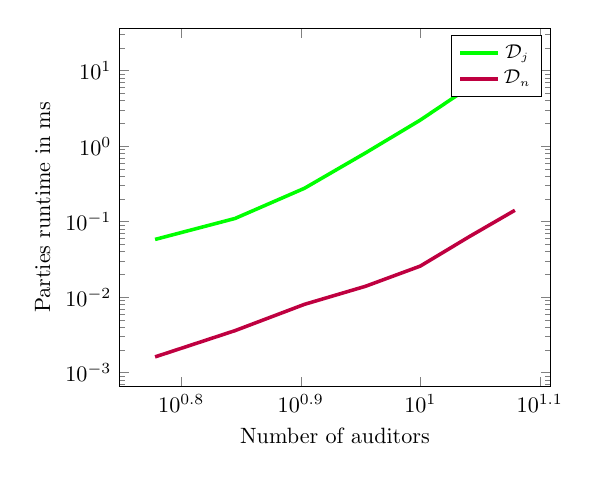
\begin{tikzpicture}[scale=.8]

\begin{loglogaxis}[
	xlabel={ Number of auditors },
	ylabel={ Parties runtime  in ms}
]


%\addplot[green,ultra thick] coordinates {
%  
%%     (1, 0.014)
%     (6, 0.033)
%     (7, 0.033)
%      (8, 0.033)
%      (9, 0.033)
%      (10, 0.033)
%      (11, 0.033)
%      (12, 0.033)
%
%};

\addplot[green, ultra thick] coordinates{

%        (1, 0.019)
       (6, 0.058)
       (7, 0.110)
      (8, 0.276)
      (9, 0.813)
      (10, 2.21)
      (11, 6.1)
      (12, 14.7)
};

\addplot[purple, ultra thick]  coordinates{

%  (1, 0.001)
        (6, 0.001611)
        (7, 0.00359)
      (8, 0.008)
      (9, 0.01389)
      (10, 0.02570)
      (11, 0.0636)
      (12, 0.141)
};


\legend{\small $\mathcal{D}_{\st j}$,\small$\mathcal{D}_{\st n}$,\small $\mathcal{DR}$}
\end{loglogaxis}
\end{tikzpicture}
\end{center}}
%\caption{\small Parties' runtime in the PwDR.}\label{plot::runtime}
%\end{figure}












% !TEX root =main.tex


\section{Future Research}


In this section, we highlight a set of future research directions in the context of APP frauds. 

\subsection{Improving Warnings' Effectiveness}

As we stated in  Section \ref{sec::Lack-of-Effective-Warning-Definition},  one of the determining factors in the process of allocating liability to APP fraud victims is if they follow warnings. However,  there exists no publicly available study on the effectiveness of warnings in  the context of APP frauds. There exists a comprehensive research line in determining the effectiveness of warnings in general, e.g., in \cite{brinton2016users,felt2014experimenting,laughery2006designing}. These traditional research line studies which factors make warnings effective and how a warning recipient is attracted to and follows the warning message. Nevertheless, in the context of APP frauds, there is a vital unique factor that can directly influence a warning's effectiveness. The factor is the ability of  fraudsters to interact directly with their victims. This lets a fraudster to actively try to negate the effectiveness of a bank's warning and persuade the warning recipient to ignore the warning (and make payment). Such a factor was not (needed to be) taken into account in the traditional study of warnings. The current high rate of  APP frauds occurrence suggests that there exists a huge room for improving warnings' effectiveness. Thus, future research can investigate (via  users studies) and identify  key factors that can improve the effectiveness of warnings in this context. 


\subsection{Protecting APP Fraud Victims of Alternative Payment Platforms}

To date, there is no official report on the occurrence of APP frauds on any other payment platforms (e.g., cryptocurrency) than  regular banking. This can be due to a lack of an oversight organisation which  collects fraud-related data or due to a low rate of such frauds taking place in these platforms because these platforms are not popular enough. Nevertheless,  with the increase in the popularity of  alternative payment platforms (including CBDC), it is likely that APP fraudsters will target these platforms' users. Hence, another interesting future research direction would be to design secure dispute resolution protocols  to protect  APP frauds victims in these platforms as well. 

\subsection{Studying Users' Compliance with the CRM Code's Guidelines}

Currently,   customers are expected to comply with the CRM code's guidelines.  Users'  compliance with these guidelines  could help lower the rate of APP frauds occurrence.  Also, if victims fail to comply with such  guidelines, then banks can claim that customers' have been negligent which ultimately could cost the victims. Such guidelines would be effective when they are known and followed by customers. Recently, Van Der Zee \cite{zee2021shifting}  has conducted an interesting study to find out whether customers of the ``Dutch Banking Association" (in the Netherlands) are aware of the bank's digital payments guidelines and if so, whether they comply with these guidelines.  But, there exists no systematic study to  investigate whether  customers are aware of and comply with the CRM code's  guidelines. Therefore, another research direction is to fill  the above void. 



\subsection{Ensuring Security Against Exploitative Victims}



Having in place a transparent deterministic procedure (e.g.,  the PwDR protocol)  for evaluating victims' requests for reimbursement  could potentially create opportunities for exploitation. In particular, an honest victim  of an APP fraud that had been reimbursed in the past due to the payment system's vulnerability (e.g., an  ineffective warning) may be tempted to  exploit the same  known vulnerability multiple times. Hence, future research can investigate how to secure the online banking system against such exploitative victims.












%!TEX root = main.tex

\section{Background}


\subsection{Existing Guideline: Contingent Reimbursement Model Code}

In  2016, the UK's consumer protection organisation, called ``Which?'', submitted a super-complaint to the FCA about  APP frauds. It raised its concerns that, despite  APP frauds victims' rate is  growing, the victims do not have enough protection \cite{Which?-super-complaint}.  Since then, the FCA has been collaborating with financial institutes  to develop several initiatives that
could help prevent these frauds, and improve the response when they  occur. As a result,  the ``Contingent Reimbursement Model'' (CRM) code has been proposed. The  CRM code  lays out a set of requirements and explains under which circumstances customers should be reimbursed by their trading financial institutes when they fall victim to an APP fraud \cite{CRM-code}. So far,  there are at least nine firms, comprising nineteen brands (e.g., Barclays, HSBC,  Lloyds) signed up to the CRM code. One of the tangible outcomes of the code is a service called ``Confirmation of Payee" (CoP)  offered by the CRM code signatories \cite{CoP}. This service checks the money recipient's account name, once it is inserted by the sender customer into the online banking platform. If there is not an exact match, CoP provides a warning to the  customers about the risks of making the payment. In the case where a customer ignores such a warning, makes a payment, and later falls to an APP fraud,  it may not be reimbursed, according to the CRM code.

Although the CRM code is a vital guideline  towards reducing the occurrence of such frauds and protecting  the frauds' victims, it is still  vague and leaves a huge room for interpretation. For instance, in 2020, the ``Financial Ombudsman Service'' (that settles complaints between consumers and businesses)  highlighted that firms  are applying the CRM code inconsistently and in some cases incorrectly, which resulted in failing to reimburse victims in circumstances anticipated by this code \cite{Financial-Ombudsman-Service-response}.  As another example, one of the conditions in the CRM code that allows a bank to avoid reimbursing the customer is clause R2(1)(e) which states: \textit{``The Customer has been grossly negligent. For the avoidance of doubt the provisions of R2(1)(a)-(d) should not be taken to define gross negligence in this context''}.  Nevertheless, neither the CRM code  nor the ``Payment Services Regulations'' \cite{Regulations}   explicitly define under which circumstances the customer is considered ``grossly negligent'' in the context of  APP frauds. In particular, in the CRM code, the only terms that discuss customers' misbehaviour are  the provisions of R2(1)(a)-(d); however, as stated above, they should be excluded from the definition of the term gross negligence. On the  other hand,  in the Payment Services Regulations, this term is used three times, i.e.,  twice in regulation 75 and once in regulation 77. But in all  three cases, it is used for frauds related to \emph{unauthorised payments} which are  different types of frauds from  APP ones. Hence, there is a pressing need for an accurate solution to help and protect  APP frauds victims. 

\subsection{Different But Related Area: Central Bank Digital Currency}

Due to the growing interest in digital payments, some central banks around the world have been exploring or even piloting the idea of ``Central Bank Digital Currency" (CBDC) \cite{CBDC}.  The idea behind CBDC is that a central bank issues digital money/token (i.e., a representation of banknotes and coins) to the public where this digital money is regulated by the nation's monetary authority or central bank, similar to regular fiat currencies. CBDC can offer various features such as efficiency, transparency, programmable money, transactions' traceability, or financial inclusion to name a few \cite{CBDC,CBDC-core-features}. Researchers have already discussed that (in CBDC) users transactions' privacy and regulatory oversight can coexist, e.g., in \cite{WustKCC19,abs-2103-00254}. In such a setting, users' amount of payments and even with whom they transact can remain confidential, while  various regulations can be accurately encoded  into cryptographic algorithms (and ultimately into a software) which are executed on users' transaction history by  authorities, e.g., to ensure compliance with ``Anti-Money Laundering'' or ``Countering the Financing of Terrorism''.  CBDC is still in its infancy and has not been adopted by banks yet. The adoption of such a model requires fundamental changes to and further digitalisations of the current banking  infrastructure. Therefore, unlike CBDC which is more futuristic, the focus of our work is on the existing regular  online banking systems.  Nevertheless, when CBDC becomes mainstream, APP frauds  might happen to the CBDC users as well. In this case, (a variant of) our result can be integrated into  such a framework to protect  APP frauds victims.  






% !TEX root =main.tex


\section{Conclusion}\label{sec::conclusion}


An APP fraud takes place when fraudsters deceive a victim to make a payment to a bank account controlled by the fraudsters. Although APP frauds have been growing at a concerning rate, the victims are not receiving a sufficient level of protection and the reimbursement rate is still low. Authorities and regulators have  provided guidelines to prevent APP frauds occurrence and improve victims’ protection, but these guidelines are still vague and open to interpretation. In this work, to facilitate APP frauds victims’ reimbursement,  we proposed the notion of payment with dispute resolution. We identified the vital properties that such a notion should possess and formally defined them. We also proposed a candidate construction,  PwDR, and proved its security.  The PwDR not only offers transparency and accountability but also acts as a data hub providing sufficient information that could help regulators examine whether the reimbursement regulations have been applied correctly and consistently among financial institutions.  We also studied the PwDR's cost via asymptotic and concrete runtime evaluation. Our cost analysis indicated that the construction is efficient. 






%Future research can investigate and identify key factors that  improve the effectiveness of banks warnings.  Furthermore, with the increase in the popularity of  alternative payment platforms (e.g., CBDC or cryptocurrency), it is likely that  fraudsters will target their users. Hence, another interesting future research direction would be to design secure dispute resolution protocols  to protect  APP frauds victims in these platforms as well. 


%Future research in this field could investigate how to design a secure protocol that could help lower the rate of APP frauds occurrence. Furthermore, with the increase in the popularity of  alternative payment platforms (such as CBDC or cryptocurrency), it is likely that APP fraudsters will target these platforms' users. Hence, another interesting future research direction would be to design secure dispute resolution protocols  to protect  APP frauds victims in these platforms as well. 




\bibliographystyle{splncs03}
\bibliography{ref}
\appendix
%% !TEX root =main.tex

%\break

\clearpage

\section{Notations}\label{sec:notation-table}

We summarise our notations in Table \ref{table:notation-table}.


\begin{table*}[!htbp]
\begin{scriptsize}
\begin{center}
\footnotesize{
\caption{ \small{Notation Table}.}\label{commu-breakdown-party} 
\renewcommand{\arraystretch}{1}
\scalebox{1.1}{
% 1st table
\begin{tabular}{|c|c|c|c|c|c|c|c|c|c|c|c|c|c|} 

\hline 

\cellcolor{gray!15} \scriptsize \textbf{Symbol}&\cellcolor{gray!15} \scriptsize \textbf{Description}  \\
    \hline
    
     \hline

%Generic
%\multirow{25}{*}{\rotatebox[origin=c]{90}{\scriptsize \textbf{Generic}}}

 \cellcolor{white!20}\scriptsize$\mathtt{Enc}(.)$&\cellcolor{white!20}\scriptsize \text{Encryption algorithm of symmetric key encryption  }\\   
 %
  \cellcolor{gray!20}\scriptsize$\mathtt{Dec}(.)$&\cellcolor{gray!20}\scriptsize \text{Decryption algorithm of symmetric key encryption  }\\   
  %
  \cellcolor{white!20}\scriptsize${\tilde{\mathtt{Enc}}}(.)$&\cellcolor{white!20}\scriptsize \text{Encryption algorithm of asymmetric key encryption  }\\   
  %
  \cellcolor{gray!20}\scriptsize${\tilde{\mathtt{Dec}}}(.)$&\cellcolor{gray!20}\scriptsize \text{Decryption algorithm of asymmetric key encryption  }\\   
  %
    \cellcolor{white!20}\scriptsize$\tilde{\mathtt{keyGen}}(.)$&\cellcolor{white!20}\scriptsize \text{Key generator algorithm of asymmetric key encryption } \\
%
   \cellcolor{gray!20}\scriptsize${\mathtt{Sig.keyGen}}(.)$&\cellcolor{gray!20}\scriptsize \text{Key generator algorithm of digital signature scheme} \\
 %
\cellcolor{white!20}\scriptsize$\mathtt{verStat}(.)$ &\cellcolor{white!20}\scriptsize  Algorithm to determine $\mathcal{B}$'s message status \\ 
%
\cellcolor{gray!20}\scriptsize$\mathtt{checkWarning}(.)$ &\cellcolor{gray!20}\scriptsize  Algorithm to check a warning’s effectiveness \\ 
%
\cellcolor{white!20}\scriptsize$\mathtt{pay}(.)$ &\cellcolor{white!20}\scriptsize $\mathcal{B}$'s internal algorithm to transfers money\\   
%
 \cellcolor{gray!20}\scriptsize$\mathtt{Com}(.)$ &\cellcolor{gray!20}\scriptsize  Commitment's commit\\
  %
\cellcolor{white!20}\scriptsize$\mathtt{Ver}(.)$ &\cellcolor{white!20}\scriptsize  Commitment's verify\\   
%                    
\cellcolor{gray!20}\scriptsize$\mathtt{H}(.)$ &\cellcolor{gray!20}\scriptsize Hash function\\
%
\cellcolor{white!20}\scriptsize$\mathtt{PRF}(.)$ &\cellcolor{white!20}\scriptsize  Pseudorandom function \\ 
%
\cellcolor{gray!20}\scriptsize$\mathcal{C}$ &\cellcolor{gray!20}\scriptsize Customer  \\  
%
\cellcolor{white!20}\scriptsize$\mathcal{B}$ &\cellcolor{white!20}\scriptsize Bank  \\
%  
\cellcolor{gray!20}\scriptsize$\mathcal{D}_{\st 1},... , \mathcal{D}_{\st n}$ &\cellcolor{gray!20}\scriptsize Arbiters  \\  
%
\cellcolor{white!20}\scriptsize$\mathcal{DR}$ &\cellcolor{white!20}\scriptsize Dispute resolver  \\  
%
\cellcolor{gray!20}\scriptsize$\mathcal{S}$ &\cellcolor{gray!20}\scriptsize Smart contract  \\  
%
\cellcolor{white!20}\scriptsize$\mathcal{G}$ &\cellcolor{white!20}\scriptsize Certificate generator  \\  
%
\cellcolor{gray!20}\scriptsize{SAP} &\cellcolor{gray!20}\scriptsize  Statement agreement protocol\\ 
%
\cellcolor{white!20}\scriptsize{PVE} &\cellcolor{white!20}\scriptsize  Private verdict encoding protocol\\ 
%
\cellcolor{gray!20}\scriptsize{FVD} &\cellcolor{gray!20}\scriptsize  Final verdict decoding protocol\\ 
%
\cellcolor{white!20}\scriptsize{GPVE} &\cellcolor{white!20}\scriptsize  Generic private verdict encoding protocol\\ 
%
\cellcolor{gray!20}\scriptsize{GFVD} &\cellcolor{gray!20}\scriptsize  Generic final verdict decoding protocol\\ 
%
\cellcolor{white!20}\scriptsize$\oplus$ &\cellcolor{white!20}\scriptsize  XOR operator \\ 
%
\cellcolor{gray!20}\scriptsize$\Delta$ &\cellcolor{gray!20}\scriptsize  time parameter \\ 
%
\cellcolor{white!20}\scriptsize$add_{\st I}$ &\cellcolor{white!20}\scriptsize  Address of $I$\\ 
%
\cellcolor{gray!20}\scriptsize$aux, aux'$ &\cellcolor{gray!20}\scriptsize  Auxiliary information\\ 
%
\cellcolor{white!20}\scriptsize$\mathtt{BF}$ &\cellcolor{white!20}\scriptsize  Bloom filter\\ 
%
\cellcolor{gray!20}\scriptsize$z_{\st 1}$ &\cellcolor{gray!20}\scriptsize  $\mathcal{C}$'s complaint about $\mathcal{B}$'s message status\\ 
%
\cellcolor{white!20}\scriptsize$z_{\st 2}$ &\cellcolor{white!20}\scriptsize  $\mathcal{C}$'s complaint about a warning's effectiveness\\
% 
\cellcolor{gray!20}\scriptsize$z_{\st 3}$ &\cellcolor{gray!20}\scriptsize  $\mathcal{C}$'s complaint about payment message  inconsistency\\ 
%
 {   }\scriptsize$t_{\st i}$ &\scriptsize  time point\\ 



                     
 \hline
  


\end{tabular}

% 2nd table
\begin{tabular}{|c|c|c|c|c|c|c|c|c|c|c|c|c|c|} 
    \hline
\cellcolor{gray!15} \scriptsize \textbf{Symbol}&\cellcolor{gray!15} \scriptsize \textbf{Description}  \\
    \hline
    
\hline


%---------------------------------
%\multirow{10}{*}{\rotatebox[origin=c]{90}{\scriptsize  \textbf{Generic}}}
%

\cellcolor{gray!20}\scriptsize$\bm{l}$ &\cellcolor{gray!20}\scriptsize  $\mathcal{C}$'s payees list\\ 
%
\cellcolor{white!20}\scriptsize$\hat{\bm{l}}$ &\cellcolor{white!20}\scriptsize  $\mathcal{C}$'s encoded payees list\\ 
%


\cellcolor{gray!20}\scriptsize$ k_{\st 0}$ &\cellcolor{gray!20}\scriptsize   A secret key of $\mathtt{PRF}$\\ 
%               
\cellcolor{white!20}\scriptsize$f$ &\cellcolor{white!20}\scriptsize New payee’s detail  \\ 
 %                            
\cellcolor{gray!20}\scriptsize$in_{\st f}$ &\cellcolor{gray!20}\scriptsize Payment detail \\ 
%
  \cellcolor{white!20}\scriptsize$\hat a$ &\cellcolor{white!20}\scriptsize Encoded $a$ \\     
%
\cellcolor{gray!20}\scriptsize$\hat {m}^{\st(\mathcal{C})}_{\st 1}$ &\cellcolor{gray!20}\scriptsize $\mathcal{C}$'s encoded update request\\     
%
\cellcolor{white!20}\scriptsize$\hat {m}^{\st(\mathcal{C})}_{\st 2}$ &\cellcolor{white!20}\scriptsize $\mathcal{C}$'s encoded payment request\\     
%      
\cellcolor{gray!20}\scriptsize$\hat {m}^{\st(\mathcal{B})}_{\st 1}$ &\cellcolor{gray!20}\scriptsize $\mathcal{B}$'s encoded warning message\\     
%
\cellcolor{white!20}\scriptsize$\hat {m}^{\st(\mathcal{B})}_{\st 2}$ &\cellcolor{white!20}\scriptsize $\mathcal{B}$'s encoded payment message\\     
%          
     \cellcolor{gray!20}\scriptsize$sk$ and $pk$ &\cellcolor{gray!20}\scriptsize Secret  and public keys\\     
%
   \cellcolor{white!20}\scriptsize$sk_{\st\mathcal{D}}$ &\cellcolor{white!20}\scriptsize Arbiters' secret key\\     
%    
\cellcolor{gray!20}\scriptsize$pp$ &\cellcolor{gray!20}\scriptsize Public parameter\\  
%
\cellcolor{white!20}\scriptsize$j$ &\cellcolor{white!20}\scriptsize  Arbiter's index,  $1\leq j\leq n$ \\ 
%
\cellcolor{gray!20}\scriptsize$T, T_{\st 1},T_{\st 2}$ &\cellcolor{gray!20}\scriptsize  Tokens, where  $T:=( T_{\st 1},T_{\st 2})$\\ 
%
\cellcolor{white!20}\scriptsize$w_{\st 1}$ &\cellcolor{white!20}\scriptsize  Output of $\mathtt{verStat}(.)$\\ 
%
\cellcolor{gray!20}\scriptsize$(w_{\st 2},w_{\st 3})$ &\cellcolor{gray!20}\scriptsize  Output of $\mathtt{checkWarning}(.)$\\ 
%
\cellcolor{white!20}\scriptsize$\bar{w}_{\st j}$ &\cellcolor{white!20}\scriptsize  Output of $\mathtt{PVE}(.)$\\ 
%
\cellcolor{gray!20}\scriptsize$v$ &\cellcolor{gray!20}\scriptsize  Output of $\mathtt{FVD}(.)$\\ 
%
\cellcolor{white!20}\scriptsize$e$ &\cellcolor{white!20}\scriptsize  Threshold\\ 
%            
 \cellcolor{gray!20}\scriptsize$w_{\st i,j}$ &\cellcolor{gray!20}\scriptsize  Arbiter's plain verdict\\ 
%     
\cellcolor{white!20}\scriptsize$o$ &\cellcolor{white!20}\scriptsize  Offset\\  
 %
  \cellcolor{gray!20}\scriptsize$r_{\st j}$ &\cellcolor{gray!20}\scriptsize  Pseudorandom value\\   
 %              
\cellcolor{white!20}\scriptsize$\lambda$ &\cellcolor{white!20}\scriptsize Security parameter\\  
%
\cellcolor{gray!20}\scriptsize$\mu$ &\cellcolor{gray!20}\scriptsize Negligible function\\  


\cellcolor{white!20}\scriptsize$in_{\st p}$ &\cellcolor{white!20}\scriptsize The input of $\mathtt{pay}(.)$\\                    
%
\cellcolor{gray!20}\scriptsize$\pi$ &\cellcolor{gray!20}\scriptsize Private statement\\        
  %
  \cellcolor{white!20}\scriptsize$Pr$ &\cellcolor{white!20}\scriptsize Probability\\   

%
\cellcolor{gray!20}\scriptsize$\phi$ &\cellcolor{gray!20}\scriptsize  Null\\ 
%
\cellcolor{white!20}\scriptsize$n$ &\cellcolor{white!20}\scriptsize  Total number of arbiters\\  
%           
\cellcolor{gray!20}\scriptsize$z$ &\cellcolor{gray!20}\scriptsize  $\mathcal{C}$'s complaint, where $z:=(z_{\st 1}, z_{\st 2}, z_{\st 3})$\\ 
%
\cellcolor{white!20}\scriptsize $g:=(g_{\st 1}, g_{\st 2})$&\cellcolor{white!20}\scriptsize  Commitment values \\    
%
%***********************

\hline 
      

           
              
\end{tabular}\label{table:notation-table}
%
}}
\end{center}
\end{scriptsize}
\end{table*}








%%%%%%%%%%%%%%%%%%%%%%%%%%%%%%%%%%%%%%%%%%%






















%% !TEX root =main.tex



\section{Bloom Filter}\label{sec::bloom-filter-}

A Bloom filter \cite{DBLP:journals/cacm/Bloom70} is a compact data structure for probabilistic efficient  elements'  membership checking. A Bloom filter is an array of $\bar  m$ bits that are initially all set to zero. It  represents $\bar n$  elements.  A Bloom filter comes along with  $\bar k$ independent hash functions. To insert an element, all the hash values of the element are computed and their corresponding bits in the filter are set to $1$. To check an element's membership, all its hash values are re-computed and checked whether all are set to one in the filter. If all the corresponding bits are one, then the element is probably in the filter; otherwise, it is not. In Bloom filters false positives are possible, i.e., it is possible that an element is not in the set, but the membership query shows that it is. According to \cite{BoseGKMMMST08}, the upper bound of the false positive probability is: $\bar q=\bar p^{\scriptscriptstyle \bar  k}(1+O(\frac{\bar k}{\bar p}\sqrt{\frac{\ln \bar m - \bar k \ln \bar  p}{\bar m}}))$,  where $\bar p$ is the probability that a particular bit in the filter is set to $1$ and calculated as: $\bar p=1-(1-\frac{1}{\bar m})^{\scriptscriptstyle \bar k\bar n}$. The efficiency of a Bloom filter depends
on  $\bar m$ and $\bar k$. The lower bound of $\bar m$  is $\bar  n \log_{\scriptscriptstyle 2}
\bar e \cdot\log_{\scriptscriptstyle 2} \frac{1}{\bar q}$, where $\bar e$ is the base of natural logarithms,  while the optimal number of hash functions is    $\log_{\scriptscriptstyle 2} \frac{1}{\bar q}$, when $\bar m$ is optimal. In this paper, we only use optimal $\bar k$ and $\bar m$. In practice, we would like to have a predefined acceptable upper bound on false positive probability, e.g., $\bar q=2^{\scriptscriptstyle - 40}$. Given $\bar q$ and $\bar n$, we can determine the rest of the parameters. 


% !TEX root =main.tex

\section{Variant 1 Encoding-Decoding Protocols Main Theorem and Proof}\label{sec::Variant-1-Theorem-proof}

\begin{reptheorem}{set-xor}
Let set $S=\{s_{\st 1},..., s_{\st m}\}$ be the union of  two disjoint subsets $S'$ and $S''$, where $S'$ contains non-zero random values pick uniformly  from a finite field $\mathbb{F}_{\st p}$, $S''$ contains zeros, $|S'|\geq c'=1$, $|S''|\geq c''=0$, and pair $(c',c'')$ is public information. Then, $r= \bigoplus\limits^{\st m}_{\st i=1} s_{\st i}$ reveals nothing beyond the public information.  
\end{reptheorem}

\begin{proof}
Let $s_{\st 1}$ and $s$, be two random values picked uniformly at random from $\mathbb{F}_{\st p}$. Let $\bar s=s_{\st 1}\oplus \underbrace{0\oplus... \oplus 0}_{\st |S''|}$. Since  $\bar s=s_{\st 1}$, two values $\bar s$ and $s$ have identical distribution. Thus, $\bar s$ reveals nothing in this case. Next, let $\tilde s=\underbrace{ s_{\st 1}\oplus s_{\st 2}\oplus... \oplus s_{\st j}}_{\st |S'|}$, where $s_{\st i}\in S'$. Since each $s_{\st i}$ is a uniformly random value,  the XOR of them is a uniformly random value too. That means values $\tilde s$ and $s$ have identical distribution. Thus, $\tilde s$ reveals nothing in this case as well. Also, it is not hard to see that the combination of the above two cases reveals nothing too, i.e., $\bar s\oplus \tilde s$ and $s$ have    identical distribution. 
%
\end{proof}
%% !TEX root =main.tex

\section{Generic Verdict Encoding-Decoding Protocols}\label{sec::Generic-Verdict-Encoding-Decoding-Protocols}

Figures \ref{fig:GPVE} and \ref{fig:GFVD} present the generic verdict encoding-decoding protocols (i.e., GPVE and GFVD), that let a semi-honest third party $\mathcal{I}$ find out if at least $e$ arbiters voted $1$, where $e$ can be any integer in the range $[1, n]$.


%
%Here, we present two efficient verdict encoding and decoding protocols; namely, Private Verdict Encoding (PVE) and Final Verdict Decoding (FVD) protocols. Their goal is to let a third party $\mathcal{I}$, e.g., $\mathcal{DR}$, find out whether at least one arbiter voted $1$, while satisfying the following  requirements.  The protocols should (1) generate unlinkable verdicts, (2)  not require arbiters to interact with each other for each customer, and (3) be  efficient. Since, the second and third requirements are self-explanatory,  we only explain the first one.  Informally, the first property requires  that the protocols should generate encoded verdicts and final verdict in a way that $\mathcal{I}$,  given the encoded verdicts and final verdict, should not be able to (a)   link a  verdict to an arbiter (except when all arbiters' verdicts are $0$), and (b) find out the total number of $1$ or $0$ verdicts when they provide different verdicts. 
%
%
%
% At a high level, the protocols work as follows.  The arbiters only once for all customers agree on a secret key of a pseudorandom function. This key will allow each of them to generate a pseudorandom masking values such that if all masking values are ``XOR''ed, they would cancel out each other and result $0$.\footnote{This is similar to the idea used in the XOR-based secret sharing \cite{Schneier0078909}.}
% 
% 
% 
% 
% 
%Each arbiter represents its verdict by (i) representing it as a parameter which is set to either $0$ if the verdict is $0$ or to a random value if the verdict is $1$, and then (ii) masking this parameter by the above  pseudorandom value.  It sends the result to $\mathcal{I}$.  To decode the final verdict and find out whether any arbiter voted $1$, $\mathcal{I}$  does XOR all encoded verdicts. This removes the masks and XORs are verdicts' representations.  If the result is $0$, then    all arbiters must have voted $0$; therefore,  the final verdict is $0$. However, if the result is not $0$ (i.e., a random value), then at least one of the arbiters voted $1$, so  the final verdict is $1$. We present the encoding  and decoding protocols in figures \ref{fig:PVE} and \ref{fig:FVD} respectively.
% 
% 
% Not that the protocols' correctness holds, except  a negligible  probability. In particular, if two arbiters  represent their verdict by an identical random value, then when they are XORed they would cannel out each other which can affect the result's correctness. The same holds if the XOR of  multiple verdicts' representations results in a value that can cancel out another verdict's representation. Nevertheless, the probability that such an event occurs is negligible in the security parameter, i.e., at most   $\frac{1}{2^{\st \lambda}}$. It is evident that PVE and FVD protocols meet properties (2) and (3). The primary reason they also meet  property (1) is that each masked verdict reveals nothing about the verdict (and its representation) and  given the final verdict, $\mathcal{I}$ cannot distinguish between the case where there is exactly one arbiter that voted  $1$ and the case where multiple arbiters voted $1$, as in both cases $\mathcal{I}$   extracts only a single random value, which reveals nothing about the number of arbiters which voted $0$ or $1$. 
% 
%  
% To encode a verdict $w$, each arbiter represents it as a polynomial. It randomises this polynomial and then  masks this polynomial with the pseudorandom masking polynomial. It sends the result to $\mathcal{I}$. To decode the final verdict and find out whether all arbiters agreed on the same verdict, i.e., unanimous decision,  $\mathcal{I}$  adds all polynomials up. This removes the masks. Next, it  evaluates the result polynomial at $v=1$ and $v=0$. It considers $v$ as the final verdict if the evaluation is  $0$. We present the encoding  and decoding protocols in figures \ref{fig:PVE} and \ref{fig:FVD} respectively. 
 



% either an specific final verdict  (i.e., $v=0$ or $v=1$) if  all arbiters' verdicts are identical, or  nothing  about the arbiters' inputs if they did not agree on the same specific verdict. The protocols are  primarily  based on ``zero-sum pseudorandom polynomials'' and the techniques often used by private set intersection (PSI) protocols. In particular, the arbiters only once for all customers agree on a secret key of a pseudorandom function. This key will allow each of them to generate a pseudorandom masking polynomial such that if all masking polynomials are summed up, they would cancel out each other and result $0$, i.e., zero-sum pseudorandom polynomials. 



%In this section, we present efficient (verdict) encoding and decoding protocols. The encoding protocol  lets each of the $n$ honest arbiters $\mathcal{D}:\{\mathcal{D}_{\st 1},..., \mathcal{D}_{\st n}\}$ non-interactively encode its verdict such that a third party party $\mathcal{I}$ (where $\mathcal{I}\notin \mathcal{D}$) can extract final verdict if  all arbiters' verdicts are identical with the following security requirements. First,  given individual encoded verdict, $\mathcal{I}$ cannot learn anything about each arbiter's verdict. Second, can find out only final verdict if  all arbiters' verdicts are identical; otherwise, it cannot learn each individual arbiter's verdict.  The decoding protocol lets  $\mathcal{I}$,  combines the encoded verdicts and learn either an specific final verdict  (i.e., $w=0$ or $w=1$) if  all arbiters' verdicts are identical, or  nothing  about the arbiters' inputs if they did not agree on the same specific verdict. The protocols are  primarily  based on ``zero-sum pseudorandom polynomials'' and the techniques often used by private set intersection (PSI) protocols. In particular, the arbiters only once for all customers agree on a secret key of a pseudorandom function. This key will allow each of them to generate a pseudorandom masking polynomial such that if all masking polynomials are summed up, they would cancel out each other and result $0$, i.e., zero-sum pseudorandom polynomials. 











%
%Below, we present ``Zero-sum Pseudorandom Values Generator'' (ZPVG), an algorithm that allows each of the $n$ arbiters  to \emph{efficiently} and \emph{independently}  generate a vector of $m$ pseudorandom values for each customer, such that when all arbiters' vectors are summed up component-wise, it would result in a vector of $m$ zeros. ZPVG is based on  the following idea. Each arbiter $\mathcal{D}_{\st j}\in\{\mathcal{D}_{\st 1},..., \mathcal{D}_{\st n-1}\}$  uses the secret key $\bar k_{\st 0}$ (as defined in Section \ref{Notations-and-Assumptions}), along with the customer's unique ID (e.g., it blockchain account's address) as the inputs of $\mathtt{PRF}(.)$  to derive $m$ pseudorandom values. However,  $\mathcal{D}_{\st n}$ generates each  $j$-th element of  its vector by computing the additive inverse of the sum of the $j$-th elements that the rest of arbiters generated. Even $\mathcal{D}_{\st n}$ does not need to interact with other arbiters, as it can regenerate their values too. Moreover, the arbiters do not need to interact with each other for every   new customer and can   reuse the same key because the new customer would have a new unique ID that would result in a fresh set of pseudorandom values (with a high probability). Figure \ref{fig:ZSPA} presents ZPVG in more detail. 





%It sends the result to all parties which can locally check if the relation holds. Note, in the literature,   there exist protocols that allows parties to agree on zero-sum pseudorandom values, e.g., in \cite{}; however, they are less efficient than $\mathtt{ZSPA}$, as their security requirements are different than ours, i.e., they assume the participants are malicious whereas we assume the arbiters who participate in this protocol  are honest. 


%Next, it commits to each value, where it uses $k_{\st 2}$ to generate the randomness of each commitment. Then, it constructs a Merkel tree on top of the commitments and  stores only the root of the tree  and the hash value of the keys (so in total three values) in  the smart contract.  Then, each party (using the keys) locally checks if the values and commitments have been constructed correctly; if so, each sends  an ``approved" message to the contract. 
%
%
%
%Informally, there are three main security requirements that $\mathtt{ZSPA}$ must meet: (a) privacy, (b)  non-refutability, and (c) indistinguishability. Privacy here means given the state of the  contract, an external party cannot learn any information about any of the (pseudorandom) values:  $z_{\st j}$; while non-refutability  means that if a party sends ``approved" then in future cannot deny the knowledge  of the values whose representation is stored in the contract. Furthermore, indistinguishability means that every $z_{\st j}$ ($1\leq j \leq m$) should be indistinguishable from a truly random value. In Fig. \ref{fig:ZSPA}, we provide $\mathtt{ZSPA}$ that efficiently generates $b$ vectors  where each vector elements is sum to zero. 



%\begin{figure}[ht]
%\setlength{\fboxsep}{0.7pt}
%\begin{center}
%\begin{boxedminipage}{12.3cm}
%\small{
%$\mathtt{ZPVG}(\bar{k}_{\st 0}, \text{ID}, n,  m, j)\rightarrow \bm r_{\st j}$\\
%------------------
%\begin{itemize}
%\item \noindent\textit{Input.} $\bar{k}_{\st 0}$: a key of  pseudorandom function's key $\mathtt{PRF}(.)$, $\text{ID}$: a unique identifier, $n$:  total number of rows of a matrix, and $m$: total number of columns of a matrix, $j$: a row's index in a matrix.
%%
%\item \noindent\textit{Output.} $\bm r_{\st j}$:  $j$-th row of an $n\times m$ matrix, such that  if $i$-th element of $\bm r_{\st j}$ is added with  the rest of elements in $i$-th column of the same matrix, the result would be  $0$. 
%\end{itemize}
%\begin{enumerate}
%%
%\item\label{ZSPA:val-gen} compute $m$ pseudorandom values as follows. 
%
%$\forall i, 1\leq i\leq m:$
%%
%\begin{itemize}
%%
%\item[$\bullet$] if $j< n: r_{\st i,j}=\mathtt{PRF}(\bar k_{\st 0}, i||j||\text{ID})$ 
%%
%\item[$\bullet$]  if $j=n: r_{\st i, n}=\big(-\sum\limits^{\st n-1}_{\st j=1} r_{\st i,j}\big) \bmod p$ 
%%
%\end{itemize}
%%
%\item return $\bm r_{\st j}=[r_{\st 1,j},..., r_{\st m,j}]$
%
%
%
%
%\
% \end{enumerate}
% 
%}
%\end{boxedminipage}
%\end{center}
%\caption{Zero-sum Pseudorandom Values Generator (ZPVG)} 
%\label{fig:ZSPA}
%\end{figure}






\begin{figure}[!ht]
\setlength{\fboxsep}{0.7pt}
\begin{center}
\begin{boxedminipage}{12.3cm}
\small{
\underline{$\mathtt{GPVE}(\bar{k}_{\st 0}, \text{ID},  w_{\st j}, o, e, n,  j)\rightarrow  (\bar{  w}_{\st j}, \mathtt{BF})$}\\
%
\begin{itemize}
\item \noindent\textit{Input.} $\bar{k}_{\st 0}$: a key of  pseudorandom function $\mathtt{PRF}(.)$, $\text{ID}$: a unique identifier, $ w_{\st j}$: a  verdict, $o$: an offset, $e$: a threshold, $n$: the total number of  arbiters,  and  $j$: an arbiter's index.
%
\item \noindent\textit{Output.} $\bar{  w}_{\st j}$:  an  encoded verdict.  
%
%$\bm r_{\st j}$:  $j$-th row of an $n\times m$ matrix, such that  if $i$-th element of $\bm r_{\st j}$ is added with  the rest of elements in $i$-th column of the same matrix, the result would be  $0$. 
\end{itemize}
Arbiter $\mathcal{D}_{\st j}$ takes the following steps.
\begin{enumerate}
%
\item\label{ZSPA:val-gen} computes a  pseudorandom  value,  as follows. 
%
%$\forall i,1\leq i\leq s:$
%
\begin{itemize}
%
\item[$\bullet$]$ \text{ if } j< n: r_{\st j}=\mathtt{PRF}(\bar k_{\st 0}, 1||o||j||\text{ID})$.\\
%
%\hspace{1mm} 
\item [$\bullet$] $ \text{ if } j=n: r_{\st j}= \bigoplus\limits^{\st n-1}_{\st i=1} r_{\st i}$.
%
\end{itemize}
Note, the above second step is taken only by $\mathcal{D}_{\st n}$.
%By the end of this phase, a random polynomial of the following form is generated, $\Psi_{\st j}=r_{\st i+2,j}\cdot x^{\st 2}+r_{\st i+1,j}\cdot x+r_{\st i,j}$.
%
\item  sets a fresh parameter, $w'_{\st j}$, that represents a verdict, as below. 
%
%$\forall i,1\leq i\leq s:$

%\begin{itemize}
%\item[$\bullet$]  $\text{ if } w_{\st j}=1:$ \text{\ sets \ } $w'_{\st j}= \alpha_{\st j}$, where $\alpha_{\st j}\stackrel{\st\$}\leftarrow \mathbb{F}_{\st p}$.
%
%\item [$\bullet$] $\text{ if } w_{\st j}=0: \text{\ sets \ } w'_{\st j}= 0$.
%
%\end{itemize}
\begin{equation*}
   w'_{\st j}= 
\begin{cases}
   0,              & \text{if } w_{\st j}=0\\
   \alpha_{\st j}=\mathtt{PRF}(\bar k_{\st 0}, 2||o||j||\text{ID}) ,& \text{if } w_{\st j}=1\\

    %0,              & \text{if } w_{\st j}=0
\end{cases}
\end{equation*}
%
\item masks  $w'_{\st j}$ as follows. %$\forall i,1\leq i\leq s:$
%
$\bar w_{\st j}= w'_{\st j}\oplus r_{\st j}$.
%
\item if $j=n$, computes a Bloom filter that encodes the combinations of verdict representations (i.e., $w'_{\st j}$)  for verdict $1$. In particular, it takes the following steps. 
\begin{itemize}
%
\item[$\bullet$] for every integer $i$ in the range $[e,n]$, computes the combinations (without repetition) of $i$ elements from set $\{\alpha_{\st 1},..., \alpha_{\st n}\}$. In the case where  multiple elements are taken at a time (i.e., $i>1$), the elements are XORed with each other. Let $W=\{(\alpha_{\st 1}\oplus... \oplus \alpha_{\st e}), (\alpha_{\st 2}\oplus ... \oplus \alpha_{\st e+1}), ..., (\alpha_{\st 1}\oplus... \oplus \alpha_{\st n})\}$ be the result.  
%
\item[$\bullet$] constructs an empty Bloom filter. Then, it inserts all elements of $W$ into this Bloom filter. Let $\mathtt{BF}$ be the Bloom filter encoding $W$'s elements. 

\end{itemize}
%

%
\item outputs ($\bar{ w}_{\st j}, \mathtt{BF})$.





%generates   a polynomial that encodes the verdict, i.e., $\Omega_{\st j}=(x-w)$.  
%
%\item multiplies the polynomial by a fresh random polynomial $\Phi_{\st j}$ of degree $1$ and adds the result with $\Psi_{\st j}$, i.e.,  $\bar\Omega_{\st j}=\Phi_{\st j}\cdot \Omega_{\st j}+\Psi_{\st j}\bmod p$. 
%
%
%\item  evaluates the result  polynomial, $\bar\Omega_{\st j}$, at every  element $x_{\scriptscriptstyle i}\in {\bm{x}}$. This yields a vector of   $y$-coordinates: $[ \bar w_{\st 1,j},..., \bar w_{\st 3,j}]$.
%%
%
%%
%\item return $\bar{\bm w}_{\st j}=[ \bar w_{\st 1,j},..., \bar w_{\st 3,j}]$.




\
 \end{enumerate}
 
}
\end{boxedminipage}
\end{center}
\caption{Generic Private Verdict Encoding  (GPVE) Protocol} 
\label{fig:GPVE}
\end{figure}
%%%%%%%%%%%%%%%%%%%%%%%%%%%%%%%%%%%%%%
%
\begin{figure}[!ht]
\setlength{\fboxsep}{0.7pt}
\begin{center}
\begin{boxedminipage}{12.3cm}
\small{
\underline{$\mathtt{GFVD}(n,  \bar{\bm w}, \mathtt{BF})\rightarrow  v$}\\
%
\begin{itemize}
\item \noindent\textit{Input.} $n$:  the total number of  arbiters,  and  $\bar{\bm w}=[\bar{ w}_{\st 1},..., \bar{ w}_{\st n}]$:  a vector of all arbiters' encodes  verdicts.
%
\item \noindent\textit{Output.} $v$: final verdict.  
%
%$\bm r_{\st j}$:  $j$-th row of an $n\times m$ matrix, such that  if $i$-th element of $\bm r_{\st j}$ is added with  the rest of elements in $i$-th column of the same matrix, the result would be  $0$. 
\end{itemize}
A third-party $\mathcal{I}$ takes the following steps.
\begin{enumerate}
%
%
\item combines  all arbiters' encoded verdicts, $\bar w_{\st j}\in \bar{\bm {w}}$, as follows. 
%
$c= \bigoplus\limits^{\st n}_{\st j=1} \bar w_{\st j}$
% $$\forall i, 1\leq i\leq 3: g_{\st i}=\sum\limits^{\st n}_{\st j=1} \bar{w}_{\st i,j} \bmod p$$
%
%\item if $n$ is odd, then sets $c=c\oplus 1$. 
%
\item checks if $c$ is in the Bloom filter, $\mathtt{BF}$. 
%
\item sets the final verdict $v$ depending on the content of $c$. Specifically, 
%
%\begin{itemize}
%%
%\item[$\bullet$] if $c=0$, sets $v=0$.
%%
%\item[$\bullet$]  otherwise, sets $v=1$.
%%
%\end{itemize}
\begin{equation*}
   v= 
\begin{cases}
    0,              &\text{if } c= 0 \text{ or } c \notin\mathtt{BF}\\
   1 ,& \text{if } c \in\mathtt{BF}\\

\end{cases}
\end{equation*}
%
\item outputs  $v$. 

\
 \end{enumerate}
 
}
\end{boxedminipage}
\end{center}
\caption{Generic Final Verdict Decoding  (GFVD) Protocol} 
\label{fig:GFVD}
\end{figure}


% !TEX root =main.tex

\section{Variant 2 Encoding-Decoding Protocol's Proof}\label{sec::Variant-2-Theorem-proof}

\begin{reptheorem}{set-bf}
Let set $S=\{s_{\st 1},..., s_{\st m}\}$ be a set of random values picked uniformly from $\mathbb{F}_{\st p}$, where the cardinality of $S$ is  public information. Let $\mathtt{BF}$ be a Bloom filter encoding all elements of   $S$. Then,  $\mathtt{BF}$ reveals nothing about any element of $S$, beyond the public information, except with a negligible probability in the security parameter, i.e., with a probability at most $\frac{|S|}{2^{\st \lambda}}$. 
\end{reptheorem}

\begin{proof}
First, we consider the simplest case where only a single element of $S$ is encoded in $\mathtt{BF}$. In this case, due to the pre-image resistance of the Bloom filter's hash functions and the fact that the set's element was picked uniformly at random from $\mathbb{F}_{\st p}$, the probability that $\mathtt{BF}$ reveals anything about the original element is at most $\frac{1}{2^{\st \lambda}}$. Now, we move on to the case where all elements of $S$ are encoded in $\mathtt{BF}$. In this case, the probability that $\mathtt{BF}$ reveals anything about at least an element of the set is $\frac{|S|}{2^{\st \lambda}}$, due to the pre-image resistance of the hash functions,  the fact that all elements were selected uniformly at random from the finite field, and the union bound. Nevertheless, when a $\mathtt{BF}$'s size is set appropriately to avoid false-positive without wasting storage, this reveals the number of elements encoded in it, which is public information.  Thus, the only information $\mathtt{BF}$ reveals is the public one.  
 %
\end{proof}
% !TEX root =main.tex
\vspace{-6mm}
\section{  (G)PVE-(G)FVD Versus Existing Voting Protocols}\label{sec:: Further-Discussion-on-the-Encoding-decoding-Protocol}
\vspace{-1mm}
%In this section, we briefly explain why  existing  solutions are not suitable replacements for the our  verdict encoding-decoding protocols. 



Each variant of our verdict encoding-decoding protocol is a voting mechanism. It  lets a third party, $\mathcal{I}$, find out if a threshold of the auditors voted $1$, while (i) generating unlinkable verdicts, (ii) not requiring auditors to interact with each other for each customer, (iii) hiding the number of $0$ or $1$ verdicts from  $\mathcal{I}$, and (iv) being  efficient. Therefore, it is natural to ask: \emph{Is there   any {e-voting} protocol, in the literature, that can  simultaneously satisfy all the above requirements?}



The short answer is no. Recently, a provably secure  e-voting protocol that can hide the number of $1$ and $0$ votes has been proposed by K{u}sters \textit{et al.} \cite{KustersL00020}. Although this scheme can satisfy the above \emph{security} requirements, it imposes a high computation cost, as  it involves computationally expensive primitives such as zero-knowledge proofs, threshold public-key encryption scheme, and generic multi-party computation. In contrast, our verdict encoding-decoding protocols rely on much more lightweight operations such as XOR and hash function evaluations.  We also  highlight that our verdict encoding-decoding protocols are in a different setting than the one in which most of the e-voting protocols are. Because the former protocols are in the setting where there exists a small number of auditors (or voters) which are trusted and can interact with each other once; whereas, the latter (e-voting) protocols are in a more  generic setting where there is a large number of  voters, some of which might be malicious, and they are not  required to interact with each other. 
%
Note that each variant of our verdict encoding-decoding protocol requires every auditor to provide an encoded vote  in order for $\mathcal{I}$ to extract the final verdict. To let each variant terminate and $\mathcal{I}$ find out the final verdict in the case where a  set of  auditors do not provide their vote, we can integrate the    following idea into each variant. We define a manager auditor, say $\mathcal{D}_{\st n}$, which is always responsive and keeps track of missing votes. After the voting time elapses and $\mathcal{D}_{\st n}$ realises a certain  number of auditors did not provide their encoded vote, it provides $0$ votes on their behalf and masks them using the  auditors' masking values. 










\end{document}






